\documentclass[letterpaper,10pt]{book}
% Change to 10 pt
\usepackage{pdfpages}
\usepackage{morewrites}			% to counteract the no write space problem
\setcounter{tocdepth}{5}

\usepackage[framemethod=TikZ]{mdframed}

\usepackage{fancyhdr}

\usepackage{paralist}
\usepackage{amsmath}
\usepackage{amsfonts}
\usepackage{amssymb}
\usepackage{graphicx}

\usepackage{datetime}
%\usepackage{ulem}

%\usepackage[nottoc]{toobibind}

\usepackage[inline]{enumitem}

% Outer margin at 2.50 is exactly correct to fit the ``corruption alert'' tables
\usepackage[inner=1.0in, outer=2.50in, top=2.54cm,bottom=2.54cm, marginparwidth=2.25in]{geometry}

\usepackage{marginnote}
\usepackage{longtable}
\usepackage{booktabs}
\usepackage{xcolor}

\usepackage{soul}

\usepackage{marginnote}
\usepackage{imakeidx} 
\usepackage[
	backref=true,
	style=numeric,
%	citestyle=numeric,
	backend=bibtex
	]{biblatex}
\usepackage[driverfallback=hypertex,colorlinks=True]{hyperref}
\usepackage{cleveref}

\makeindex[name=scripture,columnsep=20pt, columnseprule=True,columns=3, title=Scripture References]
\makeindex[name=speaker,columnsep=20pt, columnseprule=True,,columns=2, title=Sermon Creator]
\makeindex[name=series,columnsep=20pt, columnseprule=True,,columns=2, title=Sermon Series]
\makeindex[name=date,columnsep=20pt, columnseprule=True,columns=2, title=Sermon Date]

\makeindex[name=event,columnsep=20pt, columnseprule=True,columns=2, title=Event]

\makeindex[name=topic,columnsep=20pt, columnseprule=True,columns=2, title=Topic]
\makeindex[name=AWIP,columnsep=20pt, columnseprule=True,columns=3, title=All Words in Passage]
\makeindex[name=NWIV,columnsep=20pt, columnseprule=True,columns=3, title=Number of Words in Verse]
\makeindex[name=PNIP,columnsep=20pt, columnseprule=True,columns=3, title=Proper Names in Passage]
\makeindex[name=PEIP,columnsep=20pt, columnseprule=True,columns=2, title=Prophetic Events in Passage]


\makeindex[name=TWPAQ,columnsep=20pt, columnseprule=True,columns=1, title=13-Word Phrases and Quotes]
\makeindex[name=PFTTIS,columnsep=20pt, columnseprule=False,columns=3, title=Phrases found 13 times in scripture]
\makeindex[name=WFTTIS,columnsep=20pt, columnseprule=False,columns=3, title=Words found 13 times in scripture]
\makeindex[name=WFITV,columnsep=20pt, columnseprule=False,columns=3, title=Words found in exactly 13 verses]
\makeindex[name=EVENTS,columnsep=20pt, columnseprule=False,columns=2, title=Sermon Log by Place]
\makeindex[name=QUESTIONS,columnsep=20pt, columnseprule=False,columns=2, title=Bible Questions]

\makeindex[name=DOCTRINES,columnsep=20pt, columnseprule=False,columns=2, title=Doctrines]

\makeindex[name=SONGS,columnsep=20pt, columnseprule=False,columns=1, title=Songs]
\makeindex[name=LOCATION,columnsep=20pt, columnseprule=False,columns= 2, title=Location]
\makeindex[name=FACEBOOK,columnsep=20pt, columnseprule=False,columns=2, title=Facebook]

\makeindex[name=DEVOTIONAL,columnsep=20pt, columnseprule=False,columns=1, title=Devotionals]

\pagestyle{fancy}
\fancyhf{}
\fancyhead[LE,RO]{\today}
\fancyhead[RE,LO]{Notes, Outlines, Comments}
\fancyhead[CE,CO]{-page \thepage  - }

\fancyfoot[CO,CE]{\leftmark}
%\fancyfoot[LE,RO]{CSCE 692, HW1}

\title{DBR\\
Daily \\ Reads}
\author{Keith Anthony \\
\today }
%\title

%+/ffffff +   \pagenumbering{gobble}

\bibliography{Bibliographies/All20220108}

%%%%% TWEAKS:
%%% - distance from fcolorbox frame to text
\setlength{\fboxsep}{1.0pt}

\usepackage[utf8]{inputenc}
\usepackage{tikz}

%%%%%%%%%%%%%%%%%%%%%%%%%%%%%%%%%%%%%%%%%%%%%%%%%%%%%%%%%%%%%%%%%%%%%%%%%%%%%%%%

\begin{document}

\begin{titlepage}

% Set the text of the page to right-aligned until \end{flushright}
\begin{flushright}
\rightskip=-2.5cm

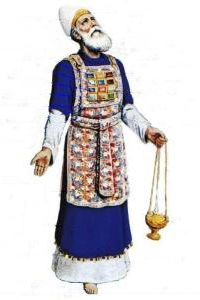
\includegraphics[width=50mm,scale=1.5]{Melchisedec.jpg}
\vspace{0.4in}

% Create a title for the document and write it in bold font
\LARGE{\textbf{\date}}
\linebreak

\vspace{0.5in}


\begin{flushleft}
\LARGE{Ruth\\}\vspace{0.25in}
\LARGE{Notes, Outlines, Comments}
\end{flushleft}

% write in large letters
%\large{Free webservices and apps}

% Skip some space
\vspace{0.6in}

%\large{Documentation}
% Skip some space

\bigskip

\normalsize{Xenia, Oh.\\}
\normalsize{created: \today}

% Skip some space
\vspace{1.3in}

\end{flushright}
% End the title page
\end{titlepage}

%\titlehttps://www.overleaf.com/project/60d732302fc633866943c9d2JE

\newpage 

\tableofcontents\hypertarget{TOC}{}
\listoffigures
\listoftables

\hyphenation{A-bim-e-lech bre-thren E-phra-im  Gib-e-o-nites Jer-u-sa-lem through-out Phil-i-stines The-o-phil-us Am-a-le-kites ven-geance Mesh-el-e-mi-ah onan-ism Phar-a-oh Py-thon thoughts grev-ous-ness Hach-a-liah adul-ter-er Shad-rach}

%\fcolorbox{black}{bone}{TEXT}
%%%%%%%%%%%%%%%%% EXTRA COLORS
%%%%%%%%%%%%%%%%% EXTRA COLORS
%%%%%%%%%%%%%%%%% EXTRA COLORS
\definecolor{champagne}{rgb}{0.97,0.91,0.81}
\definecolor{bone}{rgb}{0.89,0.85,0.79}

\definecolor{ForestGreen}{rgb}{0.00,0.29,0.098}
\definecolor{GIVING}{cmyk}{1,0.0,0.72,.1}

\definecolor{MLPE}{cmyk}{1,1,0,.45}
\definecolor{SOCCER}{cmyk}{.77, 0, .42, .49}
\definecolor{PAYBILL}{cmyk}{0,0.83,0.76,0.07}
\definecolor{SERMON}{cmyk}{.14,.9,0,.30} % aka seance \href{http://www.flatuicolorpicker.com/purple-cmyk-color-model/}{seance}
\definecolor{BIBLE}{cmyk}{0,.17,.74,.17}
\definecolor{WORKBLUE}{cmyk}{1, .5, 0, .6}
\definecolor{myOrange}{cmyk}{0, .4, .98, .03}
\definecolor{myTan}{cmyk}{0.0,.07,.17,.10}
\definecolor{myRed}{cmyk}{0,1,1,0}
\definecolor{myWhite}{cmyk}{0,0,0,0}
\definecolor{BLUESoD}{cmyk}{.97,.84,0,.04}
\definecolor{WHITE}{cmyk}{0,0,0,0}
\definecolor{OLDGOLD}{cmyk}{0.05,0.3,1.00,0}
\definecolor{CASTLETON}{cmyk}{1,0,0.31,0.66}
\definecolor{cadmiumgreen}{rgb}{0.0, 0.42, 0.24}
\definecolor{jungle}{rgb}{0.203,0.4882,0.1718}
\definecolor{MYGOLD}{rgb}{1,.84,0}

\definecolor{MYLIGHTGRAY}{rgb}{.85,.85,.85}

\definecolor{codegreen}{rgb}{0,0.6,0}
\definecolor{codegray}{rgb}{0.5,0.5,0.5}
\definecolor{codepurple}{rgb}{0.58,0,0.82}
\definecolor{backcolour}{rgb}{0.95,0.95,0.92}



\mdfdefinestyle{MyFrame}{%
    linecolor=blue,
    outerlinewidth=2pt,
    roundcorner=5pt,
    innertopmargin=\baselineskip,
    innerbottommargin=\baselineskip,
    innerrightmargin=10pt,
    innerleftmargin=10pt,
    backgroundcolor=gray!25!white}


\mdfdefinestyle{MyFrame2}{%
    linecolor=black,
    outerlinewidth=2pt,
    roundcorner=5pt,
    innertopmargin=\baselineskip,
    innerbottommargin=\baselineskip,
    innerrightmargin=10pt,
    innerleftmargin=10pt,
    backgroundcolor=yellow!25!white}



%\input{PFTTIS}
%\input{WFTTIS}
%\input{WFITV}


\chapter{Ruth 1}


\marginpar{\scriptsize \centering \fcolorbox{bone}{lime}{\textbf{COMING BACK BROKEN}}\\ (Ruth 1:1-22) \begin{compactenum}[I.][8]
    \item The \textbf{Longing} (for Food) \index[scripture]{Ruth!Ruth 01:01}(Ruth 1:1)
    \item The \textbf{Looking} (at Moab) \index[scripture]{Ruth!Ruth 01:01}(Ruth 1:1)
    \item The \textbf{Leaving} (the land of faith for the land of the flesh) \index[scripture]{Ruth!Ruth 01:01}(Ruth 1:1)
    \item The \textbf{Loosing} (husband and sons) \index[scripture]{Ruth!Ruth 01:03}\index[scripture]{Ruth!Ruth 01:05}(Ruth 1:3, 5)
    \item The \textbf{Learning} (why did she have to suffer loss to know she was in the wrong place?) 
    \item The \textbf{Listening} (why was this a surprise to her?)  \index[scripture]{Ruth!Ruth 01:06}(Ruth 1:6)
    \item Ruth's \textbf{Oblivion} (Naomi was oblivious to Ruth's faith)  %\index[scripture]{Ruth!Ruth 01:06}(Ruth 1:6)
\end{compactenum}}




\footnote{\textcolor[cmyk]{0.99998,1,0,0}{\hyperlink{TOC}{Return to end of Table of Contents.}}}\footnote{\href{https://audiobible.com/bible/ruth_1.html}{\textcolor[cmyk]{0.99998,1,0,0}{Ruth 1 Audio}}}\textcolor[cmyk]{0.99998,1,0,0}{Now it came to pass in the days when the judges ruled, that there was a \fcolorbox{bone}{lime}{famine} in the land. And a certain man of Beth-lehem-judah \fcolorbox{bone}{lime}{went} to sojourn in the country of Moab, he, and his wife, and his two sons.}
[2] \textcolor[cmyk]{0.99998,1,0,0}{And the name of the man \emph{was} Elimelech, and the name of his wife Naomi, and the name of his two sons Mahlon and Chilion, Ephrathites of Beth-lehem-judah. And they came into the country of Moab, and continued there.}
[3] \textcolor[cmyk]{0.99998,1,0,0}{And Elimelech Naomi's \fcolorbox{bone}{lime}{husband died}; and she was left, and her two sons.}
[4] \textcolor[cmyk]{0.99998,1,0,0}{And they took them wives of the women of Moab; the name of the one \emph{was} Orpah, and the name of the other Ruth: and they dwelled there about ten years.}
[5] \textcolor[cmyk]{0.99998,1,0,0}{And \fcolorbox{bone}{lime}{Mahlon and Chilion} died also both of them; and the woman was left of her two sons and her husband.}\\
\\
\P \textcolor[cmyk]{0.99998,1,0,0}{Then she arose with her daughters in law, that she might return from the country of Moab: for she had \fcolorbox{bone}{lime}{heard} in the country of Moab how that the LORD had visited his people in giving them bread.}
[7] \textcolor[cmyk]{0.99998,1,0,0}{Wherefore she went forth out of the place where she was, and her two daughters in law with her; and they went on the way to return unto the land of Judah.}
[8] \textcolor[cmyk]{0.99998,1,0,0}{And Naomi said unto her two daughters in law, Go, return each to her mother's house: the LORD deal kindly with you, as ye have dealt with the dead, and with me.}
[9] \textcolor[cmyk]{0.99998,1,0,0}{The LORD grant you that ye may find rest, each \emph{of} \emph{you} in the house of her husband. Then she kissed them; and they lifted up their voice, and wept.}
[10] \textcolor[cmyk]{0.99998,1,0,0}{And they said unto her, Surely we will return with thee unto thy people.}
[11] \textcolor[cmyk]{0.99998,1,0,0}{And Naomi said, Turn again, my daughters: why will ye go with me? \emph{are} there yet \emph{any} \emph{more} sons in my womb, that they may be your husbands?}
[12] \textcolor[cmyk]{0.99998,1,0,0}{Turn again, my daughters, go \emph{your} \emph{way}; for I am too old to have an husband. If I should say, I have hope, \emph{if} I should have an husband also to night, and should also bear sons;}
[13] \textcolor[cmyk]{0.99998,1,0,0}{Would ye tarry for them till they were grown? would ye stay for them from having husbands? nay, my daughters; for it grieveth me much for your sakes that the hand of the LORD is gone out against me.}
[14] \textcolor[cmyk]{0.99998,1,0,0}{And they lifted up their voice, and wept again: and Orpah kissed her mother in law; but Ruth clave unto her.}
[15] \textcolor[cmyk]{0.99998,1,0,0}{And she said, Behold, thy sister in law is gone back unto her people, and unto her gods: return thou after thy sister in law.}
[16] \textcolor[cmyk]{0.99998,1,0,0}{And Ruth said, Intreat me not to leave thee, \emph{or} to return from following after thee: for whither thou goest, I will go; and where thou lodgest, I will lodge: thy people \emph{shall} \emph{be} my people, and thy God my God:}
[17] \textcolor[cmyk]{0.99998,1,0,0}{Where thou diest, will I die, and there will I be buried: the LORD do so to me, and more also, \emph{if} \emph{ought} but death part thee and me.}
[18] \textcolor[cmyk]{0.99998,1,0,0}{When she saw that she was stedfastly minded to go with her, then she left speaking unto her.}
[19] \textcolor[cmyk]{0.99998,1,0,0}{So they two went until they came to Beth-lehem. And it came to pass, when they were come to Beth-lehem, that all the city was moved about them, and they said, \emph{Is} this Naomi?}
[20] \textcolor[cmyk]{0.99998,1,0,0}{And she said unto them, Call me not Naomi, call me Mara: for the Almighty hath dealt very bitterly with me.}
[21] \textcolor[cmyk]{0.99998,1,0,0}{I went out full, and the LORD hath brought me home again empty: why \emph{then} call ye me Naomi, seeing the LORD hath testified against me, and the Almighty hath afflicted me?}
[22] \textcolor[cmyk]{0.99998,1,0,0}{So Naomi returned, and Ruth the Moabitess, her daughter in law, with her, which returned out of the country of Moab: and they came to Beth-lehem in the beginning of barley harvest.}

\section{Ruth 1 Comments}

\subsection{Numeric Nuggets}
\textbf{13: } Verse 3 has 13 words.  
%\index[NWIV]{42!Ruth!Rut 1:1}\index[AWIP]{Now!Ruth!Rut 1:1}\index[AWIP]{it!Ruth!Rut 1:1}\index[AWIP]{came!Ruth!Rut 1:1}\index[AWIP]{to!Ruth!Rut 1:1}\index[AWIP]{to!Ruth!Rut 1:1 (2)}\index[AWIP]{pass!Ruth!Rut 1:1}\index[AWIP]{in!Ruth!Rut 1:1}\index[AWIP]{in!Ruth!Rut 1:1 (2)}\index[AWIP]{in!Ruth!Rut 1:1 (3)}\index[AWIP]{the!Ruth!Rut 1:1}\index[AWIP]{the!Ruth!Rut 1:1 (2)}\index[AWIP]{the!Ruth!Rut 1:1 (3)}\index[AWIP]{the!Ruth!Rut 1:1 (4)}\index[AWIP]{days!Ruth!Rut 1:1}\index[AWIP]{when!Ruth!Rut 1:1}\index[AWIP]{judges!Ruth!Rut 1:1}\index[AWIP]{ruled!Ruth!Rut 1:1}\index[AWIP]{that!Ruth!Rut 1:1}\index[AWIP]{there!Ruth!Rut 1:1}\index[AWIP]{was!Ruth!Rut 1:1}\index[AWIP]{a!Ruth!Rut 1:1}\index[AWIP]{a!Ruth!Rut 1:1 (2)}\index[AWIP]{famine!Ruth!Rut 1:1}\index[AWIP]{land!Ruth!Rut 1:1}\index[AWIP]{And!Ruth!Rut 1:1}\index[AWIP]{certain!Ruth!Rut 1:1}\index[AWIP]{man!Ruth!Rut 1:1}\index[AWIP]{of!Ruth!Rut 1:1}\index[AWIP]{of!Ruth!Rut 1:1 (2)}\index[AWIP]{Beth-lehem-judah!Ruth!Rut 1:1}\index[AWIP]{went!Ruth!Rut 1:1}\index[AWIP]{sojourn!Ruth!Rut 1:1}\index[AWIP]{country!Ruth!Rut 1:1}\index[AWIP]{Moab!Ruth!Rut 1:1}\index[AWIP]{he!Ruth!Rut 1:1}\index[AWIP]{and!Ruth!Rut 1:1}\index[AWIP]{and!Ruth!Rut 1:1 (2)}\index[AWIP]{his!Ruth!Rut 1:1}\index[AWIP]{his!Ruth!Rut 1:1 (2)}\index[AWIP]{wife!Ruth!Rut 1:1}\index[AWIP]{two!Ruth!Rut 1:1}\index[AWIP]{sons!Ruth!Rut 1:1}

\index[NWIV]{39!Ruth!Rut 1:2}\index[AWIP]{And!Ruth!Rut 1:2}\index[AWIP]{And!Ruth!Rut 1:2 (2)}\index[AWIP]{the!Ruth!Rut 1:2}\index[AWIP]{the!Ruth!Rut 1:2 (2)}\index[AWIP]{the!Ruth!Rut 1:2 (3)}\index[AWIP]{the!Ruth!Rut 1:2 (4)}\index[AWIP]{the!Ruth!Rut 1:2 (5)}\index[AWIP]{name!Ruth!Rut 1:2}\index[AWIP]{name!Ruth!Rut 1:2 (2)}\index[AWIP]{name!Ruth!Rut 1:2 (3)}\index[AWIP]{of!Ruth!Rut 1:2}\index[AWIP]{of!Ruth!Rut 1:2 (2)}\index[AWIP]{of!Ruth!Rut 1:2 (3)}\index[AWIP]{of!Ruth!Rut 1:2 (4)}\index[AWIP]{of!Ruth!Rut 1:2 (5)}\index[AWIP]{man!Ruth!Rut 1:2}\index[AWIP]{\emph{was}!Ruth!Rut 1:2}\index[AWIP]{Elimelech!Ruth!Rut 1:2}\index[AWIP]{and!Ruth!Rut 1:2}\index[AWIP]{and!Ruth!Rut 1:2 (2)}\index[AWIP]{and!Ruth!Rut 1:2 (3)}\index[AWIP]{and!Ruth!Rut 1:2 (4)}\index[AWIP]{his!Ruth!Rut 1:2}\index[AWIP]{his!Ruth!Rut 1:2 (2)}\index[AWIP]{wife!Ruth!Rut 1:2}\index[AWIP]{Naomi!Ruth!Rut 1:2}\index[AWIP]{two!Ruth!Rut 1:2}\index[AWIP]{sons!Ruth!Rut 1:2}\index[AWIP]{Mahlon!Ruth!Rut 1:2}\index[AWIP]{Chilion!Ruth!Rut 1:2}\index[AWIP]{Ephrathites!Ruth!Rut 1:2}\index[AWIP]{Beth-lehem-judah!Ruth!Rut 1:2}\index[AWIP]{they!Ruth!Rut 1:2}\index[AWIP]{came!Ruth!Rut 1:2}\index[AWIP]{into!Ruth!Rut 1:2}\index[AWIP]{country!Ruth!Rut 1:2}\index[AWIP]{Moab!Ruth!Rut 1:2}\index[AWIP]{continued!Ruth!Rut 1:2}\index[AWIP]{there!Ruth!Rut 1:2}\index[AWIP]{\emph{was}!Ruth!Rut 1:2}

\index[NWIV]{13!Ruth!Rut 1:3}\index[AWIP]{And!Ruth!Rut 1:3}\index[AWIP]{Elimelech!Ruth!Rut 1:3}\index[AWIP]{Naomi's!Ruth!Rut 1:3}\index[AWIP]{husband!Ruth!Rut 1:3}\index[AWIP]{died!Ruth!Rut 1:3}\index[AWIP]{and!Ruth!Rut 1:3}\index[AWIP]{and!Ruth!Rut 1:3 (2)}\index[AWIP]{she!Ruth!Rut 1:3}\index[AWIP]{was!Ruth!Rut 1:3}\index[AWIP]{left!Ruth!Rut 1:3}\index[AWIP]{her!Ruth!Rut 1:3}\index[AWIP]{two!Ruth!Rut 1:3}\index[AWIP]{sons!Ruth!Rut 1:3}

\index[NWIV]{31!Ruth!Rut 1:4}\index[AWIP]{And!Ruth!Rut 1:4}\index[AWIP]{they!Ruth!Rut 1:4}\index[AWIP]{they!Ruth!Rut 1:4 (2)}\index[AWIP]{took!Ruth!Rut 1:4}\index[AWIP]{them!Ruth!Rut 1:4}\index[AWIP]{wives!Ruth!Rut 1:4}\index[AWIP]{of!Ruth!Rut 1:4}\index[AWIP]{of!Ruth!Rut 1:4 (2)}\index[AWIP]{of!Ruth!Rut 1:4 (3)}\index[AWIP]{of!Ruth!Rut 1:4 (4)}\index[AWIP]{the!Ruth!Rut 1:4}\index[AWIP]{the!Ruth!Rut 1:4 (2)}\index[AWIP]{the!Ruth!Rut 1:4 (3)}\index[AWIP]{the!Ruth!Rut 1:4 (4)}\index[AWIP]{the!Ruth!Rut 1:4 (5)}\index[AWIP]{women!Ruth!Rut 1:4}\index[AWIP]{Moab!Ruth!Rut 1:4}\index[AWIP]{name!Ruth!Rut 1:4}\index[AWIP]{name!Ruth!Rut 1:4 (2)}\index[AWIP]{one!Ruth!Rut 1:4}\index[AWIP]{\emph{was}!Ruth!Rut 1:4}\index[AWIP]{Orpah!Ruth!Rut 1:4}\index[AWIP]{and!Ruth!Rut 1:4}\index[AWIP]{and!Ruth!Rut 1:4 (2)}\index[AWIP]{other!Ruth!Rut 1:4}\index[AWIP]{Ruth!Ruth!Rut 1:4}\index[AWIP]{dwelled!Ruth!Rut 1:4}\index[AWIP]{there!Ruth!Rut 1:4}\index[AWIP]{about!Ruth!Rut 1:4}\index[AWIP]{ten!Ruth!Rut 1:4}\index[AWIP]{years!Ruth!Rut 1:4}\index[AWIP]{\emph{was}!Ruth!Rut 1:4}

\index[NWIV]{21!Ruth!Rut 1:5}\index[AWIP]{And!Ruth!Rut 1:5}\index[AWIP]{Mahlon!Ruth!Rut 1:5}\index[AWIP]{and!Ruth!Rut 1:5}\index[AWIP]{and!Ruth!Rut 1:5 (2)}\index[AWIP]{and!Ruth!Rut 1:5 (3)}\index[AWIP]{Chilion!Ruth!Rut 1:5}\index[AWIP]{died!Ruth!Rut 1:5}\index[AWIP]{also!Ruth!Rut 1:5}\index[AWIP]{both!Ruth!Rut 1:5}\index[AWIP]{of!Ruth!Rut 1:5}\index[AWIP]{of!Ruth!Rut 1:5 (2)}\index[AWIP]{them!Ruth!Rut 1:5}\index[AWIP]{the!Ruth!Rut 1:5}\index[AWIP]{woman!Ruth!Rut 1:5}\index[AWIP]{was!Ruth!Rut 1:5}\index[AWIP]{left!Ruth!Rut 1:5}\index[AWIP]{her!Ruth!Rut 1:5}\index[AWIP]{her!Ruth!Rut 1:5 (2)}\index[AWIP]{two!Ruth!Rut 1:5}\index[AWIP]{sons!Ruth!Rut 1:5}\index[AWIP]{husband!Ruth!Rut 1:5}

\index[NWIV]{38!Ruth!Rut 1:6}\index[AWIP]{Then!Ruth!Rut 1:6}\index[AWIP]{she!Ruth!Rut 1:6}\index[AWIP]{she!Ruth!Rut 1:6 (2)}\index[AWIP]{she!Ruth!Rut 1:6 (3)}\index[AWIP]{arose!Ruth!Rut 1:6}\index[AWIP]{with!Ruth!Rut 1:6}\index[AWIP]{her!Ruth!Rut 1:6}\index[AWIP]{daughters!Ruth!Rut 1:6}\index[AWIP]{in!Ruth!Rut 1:6}\index[AWIP]{in!Ruth!Rut 1:6 (2)}\index[AWIP]{in!Ruth!Rut 1:6 (3)}\index[AWIP]{law!Ruth!Rut 1:6}\index[AWIP]{that!Ruth!Rut 1:6}\index[AWIP]{that!Ruth!Rut 1:6 (2)}\index[AWIP]{might!Ruth!Rut 1:6}\index[AWIP]{return!Ruth!Rut 1:6}\index[AWIP]{from!Ruth!Rut 1:6}\index[AWIP]{the!Ruth!Rut 1:6}\index[AWIP]{the!Ruth!Rut 1:6 (2)}\index[AWIP]{the!Ruth!Rut 1:6 (3)}\index[AWIP]{country!Ruth!Rut 1:6}\index[AWIP]{country!Ruth!Rut 1:6 (2)}\index[AWIP]{of!Ruth!Rut 1:6}\index[AWIP]{of!Ruth!Rut 1:6 (2)}\index[AWIP]{Moab!Ruth!Rut 1:6}\index[AWIP]{Moab!Ruth!Rut 1:6 (2)}\index[AWIP]{for!Ruth!Rut 1:6}\index[AWIP]{had!Ruth!Rut 1:6}\index[AWIP]{had!Ruth!Rut 1:6 (2)}\index[AWIP]{heard!Ruth!Rut 1:6}\index[AWIP]{how!Ruth!Rut 1:6}\index[AWIP]{LORD!Ruth!Rut 1:6}\index[AWIP]{visited!Ruth!Rut 1:6}\index[AWIP]{his!Ruth!Rut 1:6}\index[AWIP]{people!Ruth!Rut 1:6}\index[AWIP]{giving!Ruth!Rut 1:6}\index[AWIP]{them!Ruth!Rut 1:6}\index[AWIP]{bread!Ruth!Rut 1:6}

\index[NWIV]{32!Ruth!Rut 1:7}\index[AWIP]{Wherefore!Ruth!Rut 1:7}\index[AWIP]{she!Ruth!Rut 1:7}\index[AWIP]{she!Ruth!Rut 1:7 (2)}\index[AWIP]{went!Ruth!Rut 1:7}\index[AWIP]{went!Ruth!Rut 1:7 (2)}\index[AWIP]{forth!Ruth!Rut 1:7}\index[AWIP]{out!Ruth!Rut 1:7}\index[AWIP]{of!Ruth!Rut 1:7}\index[AWIP]{of!Ruth!Rut 1:7 (2)}\index[AWIP]{the!Ruth!Rut 1:7}\index[AWIP]{the!Ruth!Rut 1:7 (2)}\index[AWIP]{the!Ruth!Rut 1:7 (3)}\index[AWIP]{place!Ruth!Rut 1:7}\index[AWIP]{where!Ruth!Rut 1:7}\index[AWIP]{was!Ruth!Rut 1:7}\index[AWIP]{and!Ruth!Rut 1:7}\index[AWIP]{and!Ruth!Rut 1:7 (2)}\index[AWIP]{her!Ruth!Rut 1:7}\index[AWIP]{her!Ruth!Rut 1:7 (2)}\index[AWIP]{two!Ruth!Rut 1:7}\index[AWIP]{daughters!Ruth!Rut 1:7}\index[AWIP]{in!Ruth!Rut 1:7}\index[AWIP]{law!Ruth!Rut 1:7}\index[AWIP]{with!Ruth!Rut 1:7}\index[AWIP]{they!Ruth!Rut 1:7}\index[AWIP]{on!Ruth!Rut 1:7}\index[AWIP]{way!Ruth!Rut 1:7}\index[AWIP]{to!Ruth!Rut 1:7}\index[AWIP]{return!Ruth!Rut 1:7}\index[AWIP]{unto!Ruth!Rut 1:7}\index[AWIP]{land!Ruth!Rut 1:7}\index[AWIP]{Judah!Ruth!Rut 1:7}

\index[NWIV]{32!Ruth!Rut 1:8}\index[AWIP]{And!Ruth!Rut 1:8}\index[AWIP]{Naomi!Ruth!Rut 1:8}\index[AWIP]{said!Ruth!Rut 1:8}\index[AWIP]{unto!Ruth!Rut 1:8}\index[AWIP]{her!Ruth!Rut 1:8}\index[AWIP]{her!Ruth!Rut 1:8 (2)}\index[AWIP]{two!Ruth!Rut 1:8}\index[AWIP]{daughters!Ruth!Rut 1:8}\index[AWIP]{in!Ruth!Rut 1:8}\index[AWIP]{law!Ruth!Rut 1:8}\index[AWIP]{Go!Ruth!Rut 1:8}\index[AWIP]{return!Ruth!Rut 1:8}\index[AWIP]{each!Ruth!Rut 1:8}\index[AWIP]{to!Ruth!Rut 1:8}\index[AWIP]{mother's!Ruth!Rut 1:8}\index[AWIP]{house!Ruth!Rut 1:8}\index[AWIP]{the!Ruth!Rut 1:8}\index[AWIP]{the!Ruth!Rut 1:8 (2)}\index[AWIP]{LORD!Ruth!Rut 1:8}\index[AWIP]{deal!Ruth!Rut 1:8}\index[AWIP]{kindly!Ruth!Rut 1:8}\index[AWIP]{with!Ruth!Rut 1:8}\index[AWIP]{with!Ruth!Rut 1:8 (2)}\index[AWIP]{with!Ruth!Rut 1:8 (3)}\index[AWIP]{you!Ruth!Rut 1:8}\index[AWIP]{as!Ruth!Rut 1:8}\index[AWIP]{ye!Ruth!Rut 1:8}\index[AWIP]{have!Ruth!Rut 1:8}\index[AWIP]{dealt!Ruth!Rut 1:8}\index[AWIP]{dead!Ruth!Rut 1:8}\index[AWIP]{and!Ruth!Rut 1:8}\index[AWIP]{me!Ruth!Rut 1:8}

\index[NWIV]{30!Ruth!Rut 1:9}\index[AWIP]{The!Ruth!Rut 1:9}\index[AWIP]{LORD!Ruth!Rut 1:9}\index[AWIP]{grant!Ruth!Rut 1:9}\index[AWIP]{you!Ruth!Rut 1:9}\index[AWIP]{that!Ruth!Rut 1:9}\index[AWIP]{ye!Ruth!Rut 1:9}\index[AWIP]{may!Ruth!Rut 1:9}\index[AWIP]{find!Ruth!Rut 1:9}\index[AWIP]{rest!Ruth!Rut 1:9}\index[AWIP]{each!Ruth!Rut 1:9}\index[AWIP]{\emph{of}!Ruth!Rut 1:9}\index[AWIP]{\emph{you}!Ruth!Rut 1:9}\index[AWIP]{in!Ruth!Rut 1:9}\index[AWIP]{the!Ruth!Rut 1:9}\index[AWIP]{house!Ruth!Rut 1:9}\index[AWIP]{of!Ruth!Rut 1:9}\index[AWIP]{her!Ruth!Rut 1:9}\index[AWIP]{husband!Ruth!Rut 1:9}\index[AWIP]{Then!Ruth!Rut 1:9}\index[AWIP]{she!Ruth!Rut 1:9}\index[AWIP]{kissed!Ruth!Rut 1:9}\index[AWIP]{them!Ruth!Rut 1:9}\index[AWIP]{and!Ruth!Rut 1:9}\index[AWIP]{and!Ruth!Rut 1:9 (2)}\index[AWIP]{they!Ruth!Rut 1:9}\index[AWIP]{lifted!Ruth!Rut 1:9}\index[AWIP]{up!Ruth!Rut 1:9}\index[AWIP]{their!Ruth!Rut 1:9}\index[AWIP]{voice!Ruth!Rut 1:9}\index[AWIP]{wept!Ruth!Rut 1:9}\index[AWIP]{\emph{of}!Ruth!Rut 1:9}\index[AWIP]{\emph{you}!Ruth!Rut 1:9}

\index[NWIV]{14!Ruth!Rut 1:10}\index[AWIP]{And!Ruth!Rut 1:10}\index[AWIP]{they!Ruth!Rut 1:10}\index[AWIP]{said!Ruth!Rut 1:10}\index[AWIP]{unto!Ruth!Rut 1:10}\index[AWIP]{unto!Ruth!Rut 1:10 (2)}\index[AWIP]{her!Ruth!Rut 1:10}\index[AWIP]{Surely!Ruth!Rut 1:10}\index[AWIP]{we!Ruth!Rut 1:10}\index[AWIP]{will!Ruth!Rut 1:10}\index[AWIP]{return!Ruth!Rut 1:10}\index[AWIP]{with!Ruth!Rut 1:10}\index[AWIP]{thee!Ruth!Rut 1:10}\index[AWIP]{thy!Ruth!Rut 1:10}\index[AWIP]{people!Ruth!Rut 1:10}

\index[NWIV]{28!Ruth!Rut 1:11}\index[AWIP]{And!Ruth!Rut 1:11}\index[AWIP]{Naomi!Ruth!Rut 1:11}\index[AWIP]{said!Ruth!Rut 1:11}\index[AWIP]{Turn!Ruth!Rut 1:11}\index[AWIP]{again!Ruth!Rut 1:11}\index[AWIP]{my!Ruth!Rut 1:11}\index[AWIP]{my!Ruth!Rut 1:11 (2)}\index[AWIP]{daughters!Ruth!Rut 1:11}\index[AWIP]{why!Ruth!Rut 1:11}\index[AWIP]{will!Ruth!Rut 1:11}\index[AWIP]{ye!Ruth!Rut 1:11}\index[AWIP]{go!Ruth!Rut 1:11}\index[AWIP]{with!Ruth!Rut 1:11}\index[AWIP]{me?!Ruth!Rut 1:11}\index[AWIP]{\emph{are}!Ruth!Rut 1:11}\index[AWIP]{there!Ruth!Rut 1:11}\index[AWIP]{yet!Ruth!Rut 1:11}\index[AWIP]{\emph{any}!Ruth!Rut 1:11}\index[AWIP]{\emph{more}!Ruth!Rut 1:11}\index[AWIP]{sons!Ruth!Rut 1:11}\index[AWIP]{in!Ruth!Rut 1:11}\index[AWIP]{womb!Ruth!Rut 1:11}\index[AWIP]{that!Ruth!Rut 1:11}\index[AWIP]{they!Ruth!Rut 1:11}\index[AWIP]{may!Ruth!Rut 1:11}\index[AWIP]{be!Ruth!Rut 1:11}\index[AWIP]{your!Ruth!Rut 1:11}\index[AWIP]{husbands?!Ruth!Rut 1:11}\index[AWIP]{\emph{are}!Ruth!Rut 1:11}\index[AWIP]{\emph{any}!Ruth!Rut 1:11}\index[AWIP]{\emph{more}!Ruth!Rut 1:11}

\index[NWIV]{37!Ruth!Rut 1:12}\index[AWIP]{Turn!Ruth!Rut 1:12}\index[AWIP]{again!Ruth!Rut 1:12}\index[AWIP]{my!Ruth!Rut 1:12}\index[AWIP]{daughters!Ruth!Rut 1:12}\index[AWIP]{go!Ruth!Rut 1:12}\index[AWIP]{\emph{your}!Ruth!Rut 1:12}\index[AWIP]{\emph{way}!Ruth!Rut 1:12}\index[AWIP]{for!Ruth!Rut 1:12}\index[AWIP]{I!Ruth!Rut 1:12}\index[AWIP]{I!Ruth!Rut 1:12 (2)}\index[AWIP]{I!Ruth!Rut 1:12 (3)}\index[AWIP]{I!Ruth!Rut 1:12 (4)}\index[AWIP]{am!Ruth!Rut 1:12}\index[AWIP]{too!Ruth!Rut 1:12}\index[AWIP]{old!Ruth!Rut 1:12}\index[AWIP]{to!Ruth!Rut 1:12}\index[AWIP]{to!Ruth!Rut 1:12 (2)}\index[AWIP]{have!Ruth!Rut 1:12}\index[AWIP]{have!Ruth!Rut 1:12 (2)}\index[AWIP]{have!Ruth!Rut 1:12 (3)}\index[AWIP]{an!Ruth!Rut 1:12}\index[AWIP]{an!Ruth!Rut 1:12 (2)}\index[AWIP]{husband!Ruth!Rut 1:12}\index[AWIP]{husband!Ruth!Rut 1:12 (2)}\index[AWIP]{If!Ruth!Rut 1:12}\index[AWIP]{should!Ruth!Rut 1:12}\index[AWIP]{should!Ruth!Rut 1:12 (2)}\index[AWIP]{should!Ruth!Rut 1:12 (3)}\index[AWIP]{say!Ruth!Rut 1:12}\index[AWIP]{hope!Ruth!Rut 1:12}\index[AWIP]{\emph{if}!Ruth!Rut 1:12}\index[AWIP]{also!Ruth!Rut 1:12}\index[AWIP]{also!Ruth!Rut 1:12 (2)}\index[AWIP]{night!Ruth!Rut 1:12}\index[AWIP]{and!Ruth!Rut 1:12}\index[AWIP]{bear!Ruth!Rut 1:12}\index[AWIP]{sons!Ruth!Rut 1:12}\index[AWIP]{\emph{your}!Ruth!Rut 1:12}\index[AWIP]{\emph{way}!Ruth!Rut 1:12}\index[AWIP]{\emph{if}!Ruth!Rut 1:12}

\index[NWIV]{39!Ruth!Rut 1:13}\index[AWIP]{Would!Ruth!Rut 1:13}\index[AWIP]{ye!Ruth!Rut 1:13}\index[AWIP]{ye!Ruth!Rut 1:13 (2)}\index[AWIP]{tarry!Ruth!Rut 1:13}\index[AWIP]{for!Ruth!Rut 1:13}\index[AWIP]{for!Ruth!Rut 1:13 (2)}\index[AWIP]{for!Ruth!Rut 1:13 (3)}\index[AWIP]{for!Ruth!Rut 1:13 (4)}\index[AWIP]{them!Ruth!Rut 1:13}\index[AWIP]{them!Ruth!Rut 1:13 (2)}\index[AWIP]{till!Ruth!Rut 1:13}\index[AWIP]{they!Ruth!Rut 1:13}\index[AWIP]{were!Ruth!Rut 1:13}\index[AWIP]{grown?!Ruth!Rut 1:13}\index[AWIP]{would!Ruth!Rut 1:13}\index[AWIP]{stay!Ruth!Rut 1:13}\index[AWIP]{from!Ruth!Rut 1:13}\index[AWIP]{having!Ruth!Rut 1:13}\index[AWIP]{husbands?!Ruth!Rut 1:13}\index[AWIP]{nay!Ruth!Rut 1:13}\index[AWIP]{my!Ruth!Rut 1:13}\index[AWIP]{daughters!Ruth!Rut 1:13}\index[AWIP]{it!Ruth!Rut 1:13}\index[AWIP]{grieveth!Ruth!Rut 1:13}\index[AWIP]{me!Ruth!Rut 1:13}\index[AWIP]{me!Ruth!Rut 1:13 (2)}\index[AWIP]{much!Ruth!Rut 1:13}\index[AWIP]{your!Ruth!Rut 1:13}\index[AWIP]{sakes!Ruth!Rut 1:13}\index[AWIP]{that!Ruth!Rut 1:13}\index[AWIP]{the!Ruth!Rut 1:13}\index[AWIP]{the!Ruth!Rut 1:13 (2)}\index[AWIP]{hand!Ruth!Rut 1:13}\index[AWIP]{of!Ruth!Rut 1:13}\index[AWIP]{LORD!Ruth!Rut 1:13}\index[AWIP]{is!Ruth!Rut 1:13}\index[AWIP]{gone!Ruth!Rut 1:13}\index[AWIP]{out!Ruth!Rut 1:13}\index[AWIP]{against!Ruth!Rut 1:13}

\index[NWIV]{21!Ruth!Rut 1:14}\index[AWIP]{And!Ruth!Rut 1:14}\index[AWIP]{they!Ruth!Rut 1:14}\index[AWIP]{lifted!Ruth!Rut 1:14}\index[AWIP]{up!Ruth!Rut 1:14}\index[AWIP]{their!Ruth!Rut 1:14}\index[AWIP]{voice!Ruth!Rut 1:14}\index[AWIP]{and!Ruth!Rut 1:14}\index[AWIP]{and!Ruth!Rut 1:14 (2)}\index[AWIP]{wept!Ruth!Rut 1:14}\index[AWIP]{again!Ruth!Rut 1:14}\index[AWIP]{Orpah!Ruth!Rut 1:14}\index[AWIP]{kissed!Ruth!Rut 1:14}\index[AWIP]{her!Ruth!Rut 1:14}\index[AWIP]{her!Ruth!Rut 1:14 (2)}\index[AWIP]{mother!Ruth!Rut 1:14}\index[AWIP]{in!Ruth!Rut 1:14}\index[AWIP]{law!Ruth!Rut 1:14}\index[AWIP]{but!Ruth!Rut 1:14}\index[AWIP]{Ruth!Ruth!Rut 1:14}\index[AWIP]{clave!Ruth!Rut 1:14}\index[AWIP]{unto!Ruth!Rut 1:14}

\index[NWIV]{25!Ruth!Rut 1:15}\index[AWIP]{And!Ruth!Rut 1:15}\index[AWIP]{she!Ruth!Rut 1:15}\index[AWIP]{said!Ruth!Rut 1:15}\index[AWIP]{Behold!Ruth!Rut 1:15}\index[AWIP]{thy!Ruth!Rut 1:15}\index[AWIP]{thy!Ruth!Rut 1:15 (2)}\index[AWIP]{sister!Ruth!Rut 1:15}\index[AWIP]{sister!Ruth!Rut 1:15 (2)}\index[AWIP]{in!Ruth!Rut 1:15}\index[AWIP]{in!Ruth!Rut 1:15 (2)}\index[AWIP]{law!Ruth!Rut 1:15}\index[AWIP]{law!Ruth!Rut 1:15 (2)}\index[AWIP]{is!Ruth!Rut 1:15}\index[AWIP]{gone!Ruth!Rut 1:15}\index[AWIP]{back!Ruth!Rut 1:15}\index[AWIP]{unto!Ruth!Rut 1:15}\index[AWIP]{unto!Ruth!Rut 1:15 (2)}\index[AWIP]{her!Ruth!Rut 1:15}\index[AWIP]{her!Ruth!Rut 1:15 (2)}\index[AWIP]{people!Ruth!Rut 1:15}\index[AWIP]{and!Ruth!Rut 1:15}\index[AWIP]{gods!Ruth!Rut 1:15}\index[AWIP]{return!Ruth!Rut 1:15}\index[AWIP]{thou!Ruth!Rut 1:15}\index[AWIP]{after!Ruth!Rut 1:15}

\index[NWIV]{41!Ruth!Rut 1:16}\index[AWIP]{And!Ruth!Rut 1:16}\index[AWIP]{Ruth!Ruth!Rut 1:16}\index[AWIP]{said!Ruth!Rut 1:16}\index[AWIP]{Intreat!Ruth!Rut 1:16}\index[AWIP]{me!Ruth!Rut 1:16}\index[AWIP]{not!Ruth!Rut 1:16}\index[AWIP]{to!Ruth!Rut 1:16}\index[AWIP]{to!Ruth!Rut 1:16 (2)}\index[AWIP]{leave!Ruth!Rut 1:16}\index[AWIP]{thee!Ruth!Rut 1:16}\index[AWIP]{thee!Ruth!Rut 1:16 (2)}\index[AWIP]{\emph{or}!Ruth!Rut 1:16}\index[AWIP]{return!Ruth!Rut 1:16}\index[AWIP]{from!Ruth!Rut 1:16}\index[AWIP]{following!Ruth!Rut 1:16}\index[AWIP]{after!Ruth!Rut 1:16}\index[AWIP]{for!Ruth!Rut 1:16}\index[AWIP]{whither!Ruth!Rut 1:16}\index[AWIP]{thou!Ruth!Rut 1:16}\index[AWIP]{thou!Ruth!Rut 1:16 (2)}\index[AWIP]{goest!Ruth!Rut 1:16}\index[AWIP]{I!Ruth!Rut 1:16}\index[AWIP]{I!Ruth!Rut 1:16 (2)}\index[AWIP]{will!Ruth!Rut 1:16}\index[AWIP]{will!Ruth!Rut 1:16 (2)}\index[AWIP]{go!Ruth!Rut 1:16}\index[AWIP]{and!Ruth!Rut 1:16}\index[AWIP]{and!Ruth!Rut 1:16 (2)}\index[AWIP]{where!Ruth!Rut 1:16}\index[AWIP]{lodgest!Ruth!Rut 1:16}\index[AWIP]{lodge!Ruth!Rut 1:16}\index[AWIP]{thy!Ruth!Rut 1:16}\index[AWIP]{thy!Ruth!Rut 1:16 (2)}\index[AWIP]{people!Ruth!Rut 1:16}\index[AWIP]{people!Ruth!Rut 1:16 (2)}\index[AWIP]{\emph{shall}!Ruth!Rut 1:16}\index[AWIP]{\emph{be}!Ruth!Rut 1:16}\index[AWIP]{my!Ruth!Rut 1:16}\index[AWIP]{my!Ruth!Rut 1:16 (2)}\index[AWIP]{God!Ruth!Rut 1:16}\index[AWIP]{God!Ruth!Rut 1:16 (2)}\index[AWIP]{\emph{or}!Ruth!Rut 1:16}\index[AWIP]{\emph{shall}!Ruth!Rut 1:16}\index[AWIP]{\emph{be}!Ruth!Rut 1:16}

\index[NWIV]{29!Ruth!Rut 1:17}\index[AWIP]{Where!Ruth!Rut 1:17}\index[AWIP]{thou!Ruth!Rut 1:17}\index[AWIP]{diest!Ruth!Rut 1:17}\index[AWIP]{will!Ruth!Rut 1:17}\index[AWIP]{will!Ruth!Rut 1:17 (2)}\index[AWIP]{I!Ruth!Rut 1:17}\index[AWIP]{I!Ruth!Rut 1:17 (2)}\index[AWIP]{die!Ruth!Rut 1:17}\index[AWIP]{and!Ruth!Rut 1:17}\index[AWIP]{and!Ruth!Rut 1:17 (2)}\index[AWIP]{and!Ruth!Rut 1:17 (3)}\index[AWIP]{there!Ruth!Rut 1:17}\index[AWIP]{be!Ruth!Rut 1:17}\index[AWIP]{buried!Ruth!Rut 1:17}\index[AWIP]{the!Ruth!Rut 1:17}\index[AWIP]{LORD!Ruth!Rut 1:17}\index[AWIP]{do!Ruth!Rut 1:17}\index[AWIP]{so!Ruth!Rut 1:17}\index[AWIP]{to!Ruth!Rut 1:17}\index[AWIP]{me!Ruth!Rut 1:17}\index[AWIP]{me!Ruth!Rut 1:17 (2)}\index[AWIP]{more!Ruth!Rut 1:17}\index[AWIP]{also!Ruth!Rut 1:17}\index[AWIP]{\emph{if}!Ruth!Rut 1:17}\index[AWIP]{\emph{ought}!Ruth!Rut 1:17}\index[AWIP]{but!Ruth!Rut 1:17}\index[AWIP]{death!Ruth!Rut 1:17}\index[AWIP]{part!Ruth!Rut 1:17}\index[AWIP]{thee!Ruth!Rut 1:17}\index[AWIP]{\emph{if}!Ruth!Rut 1:17}\index[AWIP]{\emph{ought}!Ruth!Rut 1:17}

\index[NWIV]{18!Ruth!Rut 1:18}\index[AWIP]{When!Ruth!Rut 1:18}\index[AWIP]{she!Ruth!Rut 1:18}\index[AWIP]{she!Ruth!Rut 1:18 (2)}\index[AWIP]{she!Ruth!Rut 1:18 (3)}\index[AWIP]{saw!Ruth!Rut 1:18}\index[AWIP]{that!Ruth!Rut 1:18}\index[AWIP]{was!Ruth!Rut 1:18}\index[AWIP]{stedfastly!Ruth!Rut 1:18}\index[AWIP]{minded!Ruth!Rut 1:18}\index[AWIP]{to!Ruth!Rut 1:18}\index[AWIP]{go!Ruth!Rut 1:18}\index[AWIP]{with!Ruth!Rut 1:18}\index[AWIP]{her!Ruth!Rut 1:18}\index[AWIP]{her!Ruth!Rut 1:18 (2)}\index[AWIP]{then!Ruth!Rut 1:18}\index[AWIP]{left!Ruth!Rut 1:18}\index[AWIP]{speaking!Ruth!Rut 1:18}\index[AWIP]{unto!Ruth!Rut 1:18}

\index[NWIV]{34!Ruth!Rut 1:19}\index[AWIP]{So!Ruth!Rut 1:19}\index[AWIP]{they!Ruth!Rut 1:19}\index[AWIP]{they!Ruth!Rut 1:19 (2)}\index[AWIP]{they!Ruth!Rut 1:19 (3)}\index[AWIP]{they!Ruth!Rut 1:19 (4)}\index[AWIP]{two!Ruth!Rut 1:19}\index[AWIP]{went!Ruth!Rut 1:19}\index[AWIP]{until!Ruth!Rut 1:19}\index[AWIP]{came!Ruth!Rut 1:19}\index[AWIP]{came!Ruth!Rut 1:19 (2)}\index[AWIP]{to!Ruth!Rut 1:19}\index[AWIP]{to!Ruth!Rut 1:19 (2)}\index[AWIP]{to!Ruth!Rut 1:19 (3)}\index[AWIP]{Beth-lehem!Ruth!Rut 1:19}\index[AWIP]{Beth-lehem!Ruth!Rut 1:19 (2)}\index[AWIP]{And!Ruth!Rut 1:19}\index[AWIP]{it!Ruth!Rut 1:19}\index[AWIP]{pass!Ruth!Rut 1:19}\index[AWIP]{when!Ruth!Rut 1:19}\index[AWIP]{were!Ruth!Rut 1:19}\index[AWIP]{come!Ruth!Rut 1:19}\index[AWIP]{that!Ruth!Rut 1:19}\index[AWIP]{all!Ruth!Rut 1:19}\index[AWIP]{the!Ruth!Rut 1:19}\index[AWIP]{city!Ruth!Rut 1:19}\index[AWIP]{was!Ruth!Rut 1:19}\index[AWIP]{moved!Ruth!Rut 1:19}\index[AWIP]{about!Ruth!Rut 1:19}\index[AWIP]{them!Ruth!Rut 1:19}\index[AWIP]{and!Ruth!Rut 1:19}\index[AWIP]{said!Ruth!Rut 1:19}\index[AWIP]{\emph{Is}!Ruth!Rut 1:19}\index[AWIP]{this!Ruth!Rut 1:19}\index[AWIP]{Naomi?!Ruth!Rut 1:19}\index[AWIP]{\emph{Is}!Ruth!Rut 1:19}

\index[NWIV]{21!Ruth!Rut 1:20}\index[AWIP]{And!Ruth!Rut 1:20}\index[AWIP]{she!Ruth!Rut 1:20}\index[AWIP]{said!Ruth!Rut 1:20}\index[AWIP]{unto!Ruth!Rut 1:20}\index[AWIP]{them!Ruth!Rut 1:20}\index[AWIP]{Call!Ruth!Rut 1:20}\index[AWIP]{me!Ruth!Rut 1:20}\index[AWIP]{me!Ruth!Rut 1:20 (2)}\index[AWIP]{me!Ruth!Rut 1:20 (3)}\index[AWIP]{not!Ruth!Rut 1:20}\index[AWIP]{Naomi!Ruth!Rut 1:20}\index[AWIP]{call!Ruth!Rut 1:20}\index[AWIP]{Mara!Ruth!Rut 1:20}\index[AWIP]{for!Ruth!Rut 1:20}\index[AWIP]{the!Ruth!Rut 1:20}\index[AWIP]{Almighty!Ruth!Rut 1:20}\index[AWIP]{hath!Ruth!Rut 1:20}\index[AWIP]{dealt!Ruth!Rut 1:20}\index[AWIP]{very!Ruth!Rut 1:20}\index[AWIP]{bitterly!Ruth!Rut 1:20}\index[AWIP]{with!Ruth!Rut 1:20}

\index[NWIV]{32!Ruth!Rut 1:21}\index[AWIP]{I!Ruth!Rut 1:21}\index[AWIP]{went!Ruth!Rut 1:21}\index[AWIP]{out!Ruth!Rut 1:21}\index[AWIP]{full!Ruth!Rut 1:21}\index[AWIP]{and!Ruth!Rut 1:21}\index[AWIP]{and!Ruth!Rut 1:21 (2)}\index[AWIP]{the!Ruth!Rut 1:21}\index[AWIP]{the!Ruth!Rut 1:21 (2)}\index[AWIP]{the!Ruth!Rut 1:21 (3)}\index[AWIP]{LORD!Ruth!Rut 1:21}\index[AWIP]{LORD!Ruth!Rut 1:21 (2)}\index[AWIP]{hath!Ruth!Rut 1:21}\index[AWIP]{hath!Ruth!Rut 1:21 (2)}\index[AWIP]{hath!Ruth!Rut 1:21 (3)}\index[AWIP]{brought!Ruth!Rut 1:21}\index[AWIP]{me!Ruth!Rut 1:21}\index[AWIP]{me!Ruth!Rut 1:21 (2)}\index[AWIP]{me!Ruth!Rut 1:21 (3)}\index[AWIP]{home!Ruth!Rut 1:21}\index[AWIP]{again!Ruth!Rut 1:21}\index[AWIP]{empty!Ruth!Rut 1:21}\index[AWIP]{why!Ruth!Rut 1:21}\index[AWIP]{\emph{then}!Ruth!Rut 1:21}\index[AWIP]{call!Ruth!Rut 1:21}\index[AWIP]{ye!Ruth!Rut 1:21}\index[AWIP]{Naomi!Ruth!Rut 1:21}\index[AWIP]{seeing!Ruth!Rut 1:21}\index[AWIP]{testified!Ruth!Rut 1:21}\index[AWIP]{against!Ruth!Rut 1:21}\index[AWIP]{Almighty!Ruth!Rut 1:21}\index[AWIP]{afflicted!Ruth!Rut 1:21}\index[AWIP]{me?!Ruth!Rut 1:21}\index[AWIP]{\emph{then}!Ruth!Rut 1:21}

\index[NWIV]{32!Ruth!Rut 1:22}\index[AWIP]{So!Ruth!Rut 1:22}\index[AWIP]{Naomi!Ruth!Rut 1:22}\index[AWIP]{returned!Ruth!Rut 1:22}\index[AWIP]{returned!Ruth!Rut 1:22 (2)}\index[AWIP]{and!Ruth!Rut 1:22}\index[AWIP]{and!Ruth!Rut 1:22 (2)}\index[AWIP]{Ruth!Ruth!Rut 1:22}\index[AWIP]{the!Ruth!Rut 1:22}\index[AWIP]{the!Ruth!Rut 1:22 (2)}\index[AWIP]{the!Ruth!Rut 1:22 (3)}\index[AWIP]{Moabitess!Ruth!Rut 1:22}\index[AWIP]{her!Ruth!Rut 1:22}\index[AWIP]{her!Ruth!Rut 1:22 (2)}\index[AWIP]{daughter!Ruth!Rut 1:22}\index[AWIP]{in!Ruth!Rut 1:22}\index[AWIP]{in!Ruth!Rut 1:22 (2)}\index[AWIP]{law!Ruth!Rut 1:22}\index[AWIP]{with!Ruth!Rut 1:22}\index[AWIP]{which!Ruth!Rut 1:22}\index[AWIP]{out!Ruth!Rut 1:22}\index[AWIP]{of!Ruth!Rut 1:22}\index[AWIP]{of!Ruth!Rut 1:22 (2)}\index[AWIP]{of!Ruth!Rut 1:22 (3)}\index[AWIP]{country!Ruth!Rut 1:22}\index[AWIP]{Moab!Ruth!Rut 1:22}\index[AWIP]{they!Ruth!Rut 1:22}\index[AWIP]{came!Ruth!Rut 1:22}\index[AWIP]{to!Ruth!Rut 1:22}\index[AWIP]{Beth-lehem!Ruth!Rut 1:22}\index[AWIP]{beginning!Ruth!Rut 1:22}\index[AWIP]{barley!Ruth!Rut 1:22}\index[AWIP]{harvest!Ruth!Rut 1:22}


\section{Ruth 1 Outlines}

\subsection{My Outlines}

\subsubsection{Coming Back Broken}
\index[speaker]{Keith Anthony!Ruth 01 (Coming Back Broken)}
\index[series]{Ruth (Keith Anthony)!Ruth 01 (Coming Back Broken)}
\index[date]{2017/03/21!Ruth 01 (Coming Back Broken) (Keith Anthony)}
\textbf{Introduction: }Naomi's return to Bethlehem pictures Israel return back to the land during the church Age. She comes back bitter and broken, but gets blessed by her connection to Ruth and Boaz. Later she gets to witness a wedding between the two!
\begin{compactenum}[I.][7]
    \item The \textbf{Longing} (for food) \index[scripture]{Ruth!Ruth 01:01}(Ruth 1:1)
    \item The \textbf{Looking} (at Moab) \index[scripture]{Ruth!Ruth 01:01}(Ruth 1:1)
    \item The \textbf{Leaving} (the land of faith for the land of the flesh) \index[scripture]{Ruth!Ruth 01:01}(Ruth 1:1)
    \item The \textbf{Loosing} (husband and sons) \index[scripture]{Ruth!Ruth 01:03}\index[scripture]{Ruth!Ruth 01:05}(Ruth 1:3, 5)
    \item The \textbf{Learning} (why did she have to suffer loss to know she was in the wrong place?) 
    \item The \textbf{Listening} (why was this a surprise to her?)  \index[scripture]{Ruth!Ruth 01:06}(Ruth 1:6)
    \item Ruth's \textbf{Oblivion} (Naomi was oblivious to Ruth's faith)  %\index[scripture]{Ruth!Ruth 01:06}(Ruth 1:6)
\end{compactenum}



\subsection{Outlines from Others}

\subsubsection{Three Tombstones in a Washpot}
\index[speaker]{unknown!Ruth 01:01-07 (Three Tombstones in a Washpot)}
\index[series]{Ruth (unknown)!Ruth 01:01-07 (Three Tombstones in a Washpot)}
\index[date]{unknown!Ruth 01:01-07 (Three Tombstones in a Washpot) (unknown)}
\textbf{Source: }sermonnotebook.org\\
\textbf{Introduction: }The little book of Ruth has been called ``the greatest piece of literature ever written.'' Another writer called the story of Ruth ``the Cinderella of the Bible.'' It is the story of how a pagan girl named Ruth came to be part of the covenant people of Israel. In the 100 verses that make up the book of Ruth, we see this young woman as she is pursued by grace, and brought out of her wretched condition. This is a story of redemption, of love, of grace and of hope. It is a story we need to become familiar with on a very intimate level.  n these first seven verses of Ruth we are introduced to the family of a man named Elimelech who lived during the days of the judges, v. 1. It is the sad tale of a man who chooses to walk out on the Lord and on God's plan for his life. As a result of his decision, he and his family pay a terribly high price. We are told that Elimelech takes his family to a place called Moab. Moab was located just across the Jordan River, east of the Promised Land. It was inhabited by people who worshiped pagan gods. The Moabites were the descendants of a man named Moab who was the son of an incestuous relationship between Lot and on of his daughters, Gen. 19:30-38. They were a proud people noted for their lawlessness, immorality and brutal violence, Lev. 18:24--25; Deut. 9:4--5; Isa. 16:6; Psa. 60:8. They attacked and opposed Israel, seeking to destroy the people of God, during Israel's wilderness wanderings, Num. 23--25; Deut. 23:3---6. This was a people opposed to God and His ways. In Psalm 60:8, God says this, ``Moab is my washpot $\hdots$ '' This phrase means that they were a despised thing, compared to a vessel containing water to be used by slaved to wash the feet of a conquering hero. God says that they are nothing and that they will be reduced to the lowest form of slavery! Yet, they were a people who could have been saved had they repented of their sins as Ruth did. It is to this despised and wicked nation that Elimelech moves his family. Here we see a picture of that person who willingly turns his back on the things of God and pays an awful price. If this section of scripture teaches us anything, it teaches us that living in a backslidden condition carries with it devastating consequences, but repentance and restoration are always a possibility. With this information in mind today, let's look into this passage of scripture today as I preach on the thought Three Tombstones In A Washpot.
\begin{compactenum}[I.][7]
    \item A Time of \textbf{Desperate Circumstances} \index[scripture]{Ruth!Ruth 01:01}(Ruth 1:1)
    \begin{compactenum}[A.][7]
    	\item A \textbf{Material Famine} in the Land -- Verse 1 describes the situation that Elimelech and his family faced by telling us that there was ``a famine in the land.'' A famine is an extended dearth. A time when food is in serious shortage. While there was a shortage of foods in the land at that time, it wasn't the only famine the people of Israel faced.
    	\item A \textbf{Moral Famine} in the Land -- Verse 1 tells us that this story takes place during the time of the Judges. The attitude of the people during those days is summed up in the last verse of the book of Judges, Judges 21:25. It can best be described as a time of turbulence and social upheaval. They were days marked by lawlessness, idolatry, false religion, theft, drunkenness, homosexuality, sexual perversion, violence, national division, civil war and extreme unbelief. Days, it would see, that are not too different from the days in which we find ourselves. Of course, when man ``does that which is right in his own eyes'', what else should we expect?
    	\item A \textbf{Missionary Famine} in the Land  -- 	Often, in the Old Testament period, God used famine as a tool of discipline. When His people strayed away from Him, He would reach out to them to call them back to Himself by orchestrating a famine, Deut. 11:16-17; ; 2 Chron. 7:13-14.
    \end{compactenum}
	\item A Time of \textbf{Dangerous Choices} \index[scripture]{Ruth!Ruth 01:02}(Ruth 1:2)
    \begin{compactenum}[A.][7]
    	\item Choose to \textbf{Leave the Promised Land} -- Verse 1 tells us that this man made a conscious decision to leave ``Bethlehem-Judah'' for the country of Moab. The name ``Bethlehem'' means ``House of Bread'' and the name ``Judah'' means ``Praise''. At the present time neither of those places were living up to their names. There was no bread in "The House Of Bread" and there was no reason for rejoicing in "Praise". However, while the geographic locations failed to live up to their names, so did Elimelech! His name means "My God Is King." If that had been true about this man, he would have known that God's valleys do not last forever and that God would have taken care of His people. After all, Elimelech had a close relative name Boaz. He stayed in Bethlehem and seemed to do quite well in spite of the famine, Ruth 2:1. Yet, Elimelech chose to leave his inheritance in the promised land and head off to a land where God would not bless him!
    	\item Choose to \textbf{Live in a Polluted Land} -- To leave Israel to go to Moab was to violate the clear commandment of the Lord, Josh. 23:7, 12. Yet, Elimelech chose the forbidden path to Moab over contentment in the things of the Lord. To leave one's inheritance as Elimelech did was equivalent to denying the faith of Jehovah. It was a total turning from God to the world. You see, for Elimelech and his family, this move to Moab involved total separation from the things of God. They could not worship at the Temple, they could not bring their offerings, they could keep the feasts that were commanded by the Law. They were totally isolated from everything that stood for God. Not only that, by moving his family to Moab, Elimelech exposed his family to evils they would have avoided had they stayed in Israel. For instance, both of those boys married pagan women. It is never right for a child of God to marry an unbeliever, 2 Cor. 6:14. These men violated the will of God by intermingling with this pagan race, Ezra 9:1-2; Neh. 13:23.
    	\item Choose to \textbf{Linger in a the Prodigal Land} -- This family went to Moab and there they stayed! The word "continued" means "to exist or to become." This may indicate that not only did Elimelech and his family go into Moab, but that Moab got into them as well. Who knows how far into the sin and society of Moab this family fell. I am sure when they left they told themselves that it would only last a short time. But the days turned into weeks, the weeks into months and the months into years. Before they knew it, 10 years had passed, v. 4, and they were farther away from the Lord than could have ever imagined themselves being.
    \end{compactenum}
     \item A Time of \textbf{Deadly Consequences} \index[scripture]{Ruth!Ruth 01:03--05}(Ruth 1:3--5)
    \begin{compactenum}[A.][7]
    	\item There was \textbf{Discipline} in that Home -- Before Elimelech loaded up his family to move to Moab, it is likely that he had already moved away from God in his heart. You see, no one just wakes up one morning and decides to leave God behind! It is a slow subtle process that builds until the believer has moved farther away from the Lord than he could have ever anticipated. The reason I say there was discipline in that home lies in the names of Elimelech's sons. There names were Mahlon which means "Sick" and Chilion which means "Pining, or Wasting Away." It may be that these two boys were just the victims of circumstance. But, if you believe that, then you don't believe in a God of providence! I think God was trying to get Elimelech's attention long before he ever left for Moab.
     	\item There was \textbf{Death} in that Home -- In spite of his relationship to the Lord, in spite of the blessings of God, in spite of the intervention of the Lord in his family, Elimelech moved to Moab. What was a reality in his heart became a reality in his life! After he was there for some time, he died. After a while, his sons were also taken in death. It is my opinion that God used the ultimate form of discipline in the lives of Elimelech and his family in order to bring the remainder of the family back to God. You see, the famine in Bethlehem was a call to repent. Those sick sons were a call to repent. God gave this family ten years of rope, but time finally ran out and they paid the ultimate price for their disobedience.
    	\item There was \textbf{Defeat} in that Home -- Naomi and her two daughters-in-law were left desolate. In that society, the poorest of the poor were widows with no children to care for them. These women were left with nothing but desolation, discouragement and defeat. It didn't have to be, but because of the sin in their hearts and the choices they made in life, they were forced to pay a horrible price. All Naomi had to show for her disobedience and backsliding were three tombstones in the land of Moab. All she had left were her daughters-in-law and she couldn't even provide for them. These women were in a desperate condition.
   \end{compactenum}
        \item A Time of \textbf{Deliberate Changes} \index[scripture]{Ruth!Ruth 01:03--05}(Ruth 1:3--5)
    \begin{compactenum}[A.][7]
    	\item a Time of \textbf{Realization}  -- Somehow or another Naomi heard that the Lord was again blessing His people. In truth, He had never stopped blessing! Did you know His chastisement is also His blessing? If he didn't love you He would chastise you when you failed. Anyway, someone came into Moab with the good news that God was blessing back in Israel. This sparked a desire in her heart to go home. Maybe she remembered what it was like to be close to the things of God. Maybe she remembered the sacrifices and the worship. Maybe she missed the sweet fellowship she had enjoyed with the people of God. Whatever the thoughts were that went through her head, she finally woke up in Moab and wanted to go home. This is what happened to the Prodigal Son, Luke 15:17, "And when he came to himself..." (Ill. Being in a Backslidden condition is a form of insanity.) When that boy saw where he was and what he was missing out on, he wanted to go home. So it was with Naomi.
   		\item a Time of \textbf{Repentance}  -- The Bible says that she "Arose...that she might return from the country of Moab", v. 6; and "Wherefore she went out of the place where she was..." Naomi rose up and left Moab behind! She experienced a change of heart that resulted in a change of action. She is a picture of someone repenting of their time in Moab and returning home.
   		\item a Time of \textbf{Returning}  -- Naomi rose up and went on her way to return to the land of Judah. She was headed back to the land of "Praise". She was going back to where she should have been all along! She was going home!
   \end{compactenum}
\end{compactenum}
\textbf{Conclusion: }When Naomi went into Moab, by her own testimony, she went in full, Ruth 1:21. When she came out, she came out empty. All of her hopes, all of her dreams and all of her to morrows were reduced to three tombstones in a washpot called Moab. When she left that country she left everything she valued behind. When you go to Moab, you always leave something! Naomi left three tombstones in her Moab, what will you leave behind? Will you leave you testimony? Will you leave you innocence? Will you leave your health? Will you leave your wealth? Will you leave you family? What will your journey away from God cost you? Whatever it is, it will cost less to come home today than it will if you wait to a later date. You will leave less behind if you come now than if you wait until later. God can salvage more from your life now than He can if you linger in that polluted country. By the way lost friend, this message is for you too! God is calling you to leave your wretched life of sin behind and to come to Him and be saved. If you linger there away from Him, you will pay the ultimate price. You will lose your soul in Hell! It doesn't have to be that way. If the Lord is calling you to be saved, get to Him today and let Him take care of that for you!


\subsubsection{Ruth's Journey}
\index[speaker]{unknown!Ruth 01 (Ruth's Journey -- Example of a Steadfast Life)}
\index[series]{Ruth (unknown)!Ruth 01 (Ruth's Journey -- Example of a Steadfast Life)}
\index[date]{unknown!Ruth 01 (Ruth's Journey -- Example of a Steadfast Life) (unknown)}
\textbf{Source: }sermonnotebook.org\\
\textbf{Introduction: }There are many stories in the Bible that serve as an encouragement to our hearts. The story of Ruth is no exception. Many look at this little book, which was written during the time if the judges, and see nothing more than a love story. However, while there is a love story of sorts in this book, that is the most shallow interpretation. The bigger picture is that of a lost sinner who, through divine guidance and providence, is brought into a relationship with Jehovah and is made to be an ancestor of the Lord Jesus Christ. We are taught in this book that God is not just the Savior of Israel, but that He is the Savior of the entire human race!
I wish there was time this evening to preach this entire book tonight, but there isn't. What I would like to do is to look into the verses we have read this evening and pull out a little snapshot of the heart of this woman named Ruth. In these verses, and throughout this book as well, we see in Ruth a tremendous example of a steadfast life. She teaches us about remaining faithful even when others around us do not. As we have time this evening, let's look into these verses and examine this Example Of A Steadfast Life.%\footnote{From http://www.sermonnotebook.org/old testament/Ruth 1_1-22.htm}
\begin{compactenum}[I.][7]
    \item Ruth's \textbf{Condition} \index[scripture]{Ruth!Ruth 01:01--07}(Ruth 1:1--7)
    \begin{compactenum}[A.][7]
    	\item Her Ancestry \index[scripture]{Ruth!Ruth 01:04}(Ruth 1:4) -- Ruth was a member of a condemned nation. She and her people were sinful and had been judged and condemned by the Lord. Her's was a desperate and lost condition.
    	\item her Adversity \index[scripture]{Ruth!Ruth 01:05}(Ruth 1:5) -- This verse tells us that Naomi's husband and his brother both have died. These young women are left widows with no means of support and with no hope for the future. They faced a terrible trial. It seemed that there only hope was to return to the home of their father and hope another man would eventually marry them.
    	\item Her Ambition \index[scripture]{Ruth!Ruth 01:06-07}(Ruth 1:6--7) -- Naomi has heard that the famine that caused her family to leave Bethlehem to begin with has ended and that there is bread in the land. So, she rises up to go home, and her two daughter-in-laws rise up to go with her.
    \end{compactenum}
    \item Ruth's \textbf{Challenge} \index[scripture]{Ruth!Ruth 01:08--15}(Ruth 1:8--15)
    \begin{compactenum}[A.][7]
    	\item An Expectation \index[scripture]{Ruth!Ruth 01:08-09}(Ruth 1:8--9) -- As they begin their journey, Naomi encourages both of these girls to return to the home of their mothers. She prays that the Lord will bless them, but she intends to send them away. Such is the condition of Naomi's heart that she would try to keep these women from going with her into the promised land of blessing.
    	\item An Explanation \index[scripture]{Ruth!Ruth 01:10-13}(Ruth 1:10--13) -- Naomi tries to persuade these women to go home because she has no more sons to marry the women and give them children under the law of the Levirate Marriage. And, even if she remarried and had children, these girls couldn't be expected to wait until these new sons were grown.
    	\item An Evacuation \index[scripture]{Ruth!Ruth 01:14}(Ruth 1:14) -- When Orpah heard this speech, she kissed her mother-in-law and turned around and went home.
    	\item An Examination \index[scripture]{Ruth!Ruth 01:14}(Ruth 1:14) -- After Orpah leaves, Ruth clings to Naomi. She is determined to stay with her mother-in-law. This allows us a glimpse into her heart. She shows us, by here actions that which is the best response in a time of challenge. The heart Ruth reveals to us is one of absolute devotion and commitment. You see, instead of driving us away from our commitments, the challenges of life should cause us to cleave to Him more strongly. In her commitment, Ruth demonstrates the fact that her heart had been changed and she was willing to follow a new Lord into a new land to live a new life.)
    \end{compactenum}
    \item Ruth's \textbf{Commitment} \index[scripture]{Ruth!Ruth 01:16--22}(Ruth 1:16--22)
    \begin{compactenum}[A.][7]
    	\item She Commits to a New Land \index[scripture]{Ruth!Ruth 01:16}(Ruth 1:16) -- She is willing to follow Naomi where ever she goes. She is willing to leave Moab behind forever and to follow Naomi to Israel.
    	\item She Commits to New Leadership \index[scripture]{Ruth!Ruth 01:16}(Ruth 1:16) -- She is willing to submit to Naomi and to allow Naomi to guide her life. (Ill. This is seen in the various times that Naomi gives Ruth advise concerning the manners and customs of Israel.)
    	\item She Commits to a New Lineage \index[scripture]{Ruth!Ruth 01:16}(Ruth 1:16) -- Ruth is willing to cut all ties with Moab. She wants to be a part of the nation which she has married into. She is ready to claim a new lineage.
    	\item She Commits to a New Lord \index[scripture]{Ruth!Ruth 01:16}(Ruth 1:16) -- This is perhaps the greatest statement Ruth makes. She is willing to give up the gods of Moab and follow the true and living God of Israel. This statement is her declaration of faith in Jehovah God.
    	\item She Commits with No Limits \index[scripture]{Ruth!Ruth 01:16}(Ruth 1:16) -- She tells Naomi that she is willing to commit to this new plan for life for as long as she lives. She even invokes the curse of God upon her life if she lets anything but death come between her and the commitment she has made.
    \end{compactenum}
\end{compactenum}
\textbf{Conclusion: }Ruth lived a consistent and steadfast life. She was brought into Israel, married an Israelite man named Boaz and became a part of the covenant people of the Lord. She became the great-grandmother to King David and an ancestor of the Lord Jesus Christ. All of this came to pass in her life because she was unwilling to change her mind, change her devotion or to change her direction. She kept on going in the face of adversity and she did not give up. Can the same be said about you this evening? Are you living a life that is steadfast and unmoveable, always abounding in the work of the Lord, 1 Cor. 15:58? Or has your devotion to the Lord tended to fluctuate with the changing tides of life? You know, you need God today, but you don't serve Him tomorrow. Where is your heart tonight? Are you more like Orpah who chose the easy path? Or, are you like Ruth who persevered through her difficulties to win the ultimate victory of faith? Are there issues that you need to get settled with the Lord this evening? If so, this altar is open for your use. Please use it as the Lord leads.

\subsubsection{The Massacre at Moab}
\index[speaker]{Donald Cantrell!Ruth 01:01-05 (The Massacre at Moab)}
\index[series]{Ruth (Donald Cantrell)!Ruth 01:01-05 (The Massacre at Moab)}
\index[date]{unknown!Ruth 01:01-05 (The Massacre at Moab)}
\textbf{Source: }www.sermonsearch.com\\
\textbf{Speaker: }Donald Cantrell\\
\begin{compactenum}[I.][7]
    \item The \textbf{The Destructive Decision} \index[scripture]{Ruth!Ruth 01:01}(Ruth 1:1)
    \begin{compactenum}[A.]
    	\item The \textbf{Mounting Famine} 
    	\item The \textbf{Mentioned Family} 
    	\item The \textbf{Moab Flight} 
    \end{compactenum}
    \item The \textbf{The Descriptive Destination} \index[scripture]{Ruth!Ruth 01:02}(Ruth 1:2)
    \begin{compactenum}[A.]
    	\item The \textbf{Jewish People} 
    	\item The \textbf{Jeopardous Place} 
    \end{compactenum}
    \item The \textbf{The Deadly Destination} \index[scripture]{Ruth!Ruth 01:03}(Ruth 1:3)
    \begin{compactenum}[A.]
    	\item The \textbf{Elimelech's Departure} 
    	\item The \textbf{Elimelech's Descendants} 
    \end{compactenum}
    \item The \textbf{The Delayed Demolition} \index[scripture]{Ruth!Ruth 01:04-05}(Ruth 1:4-5)
    \begin{compactenum}[A.]
    	\item The \textbf{Lengthy Dwelling} of the Men \index[scripture]{Ruth!Ruth 01:04}(Ruth 1:4)
    	\item The \textbf{Literal Death} of the Men \index[scripture]{Ruth!Ruth 01:05}(Ruth 1:5)
    \end{compactenum}
\end{compactenum}

\subsubsection{Decisions, Departing, and Dedication}
\index[speaker]{Donald Cantrell!Ruth 01:06-18 (Decisions, Departing, and Dedication)}
\index[series]{Ruth (Donald Cantrell)!Ruth 01:06-18 (Decisions, Departing, and Dedication)}
\index[date]{unknown!Ruth 01:06-18 (Decisions, Departing, and Dedication) (Donald Cantrell)}
\textbf{Source: }www.sermonsearch.com\\
\textbf{Speaker: }Donald Cantrell\\
\begin{compactenum}[I.][7]
    \item \textbf{Naomi's Favorable Decision and Aim} \index[scripture]{Ruth!Ruth 01:06-18}(Ruth 1:6-18)
	\begin{compactenum}[A.]
	    	\item The \textbf{Glorious Report} \index[scripture]{Ruth!Ruth 01:06}(Ruth 1:6)
    	\item The \textbf{Gracious Response} \index[scripture]{Ruth!Ruth 01:07}(Ruth 1:7)
    	\item The \textbf{Grievous Request} \index[scripture]{Ruth!Ruth 01:08-13}(Ruth 1:8-13)
	\end{compactenum}
    \item \textbf{Orpah's Foolish Departure and Abandonement} \index[scripture]{Ruth!Ruth 01:14a, 15}(Ruth 1:14a, 15)
    	\begin{compactenum}[A.]
    		\item Orpah's \textbf{Divided Heart} \index[scripture]{Ruth!Ruth 01:06}(Ruth 1:6)
    		\begin{compactenum}[1.]
    			\item Her \textbf{Family and Relatives}
    			\item Her \textbf{Faith and Religion}
    		\end{compactenum}
	    	\item Orpah's \textbf{Deadly Hour} \index[scripture]{Ruth!Ruth 01:06}(Ruth 1:6)
    		\begin{compactenum}[1.]
    			\item Her \textbf{False Profession}
    			\item Her \textbf{Final Place}
    		\end{compactenum}
		\end{compactenum}
    \item \textbf{Ruth's Faithful Devotion and Affection} \index[scripture]{Ruth!Ruth 01:14b, 16-18}(Ruth 1:14b, 16-18)
    	\begin{compactenum}[A.]
    		\item Ruth \textbf{Mightily Clinging} \index[scripture]{Ruth!Ruth 01:14b}(Ruth 1:14b)
    		\begin{compactenum}[1.]
    			\item Her \textbf{Tight Hold}
    			\item Her \textbf{Tender Heart}
    		\end{compactenum}
	    	\item Ruth \textbf{Majestically Confessing} \index[scripture]{Ruth!Ruth 01:16-18}(Ruth 1:16-18)
    		\begin{compactenum}[1.]
    			\item Her \textbf{Pointed Course Profession} \index[scripture]{Ruth!Ruth 01:16a}(Ruth 1:16a)
    			\item Her \textbf{Personal Choice} \index[scripture]{Ruth!Ruth 01:16b}(Ruth 1:16b)
    			\item Her \textbf{Parting Claim} \index[scripture]{Ruth!Ruth 01:17a}(Ruth 1:17a)
    			\item Her \textbf{Phenomenal Change} \index[scripture]{Ruth!Ruth 01:17b-18}(Ruth 1:17b-18)
    		\end{compactenum}
		\end{compactenum}
\end{compactenum}



\subsubsection{Ruth's Journey}
\index[speaker]{Donald Cantrell!Ruth 01:19-22 (Ruth's Journey -- Example of a Steadfast Life)}
\index[series]{Ruth (Donald Cantrell)!Ruth 01:19-22 (Ruth's Journey -- Example of a Steadfast Life)}
\index[date]{unknown!Ruth 01:19-22 (Ruth's Journey -- Example of a Steadfast Life) (Donald Cantrell)}
\textbf{Source: }www.sermonsearch.com\\
\textbf{Speaker: }Donald Cantrell\\
\begin{compactenum}[I.][7]
    \item The \textbf{Notable City} \index[scripture]{Ruth!Ruth 01:19a}(Ruth 1:19a)
    \item The \textbf{Noisy Conversation} \index[scripture]{Ruth!Ruth 01:19b}(Ruth 1:19b)
    \item The \textbf{Numbing Cry} \index[scripture]{Ruth!Ruth 01:20}(Ruth 1:20)
    \item The \textbf{Negated Calculation} \index[scripture]{Ruth!Ruth 01:21}(Ruth 1:21)
    \item The \textbf{New Course} \index[scripture]{Ruth!Ruth 01:22}(Ruth 1:22)
\end{compactenum}

%\section{Ruth 1 Statistics}

%%%%%%%%%%%%%%%%%%%%%%%%%%%
%%%%% Word Statistics
%%%%%%%%%%%%%%%%%%%%%%%%%%


\normalsize



\subsection{Chapter Word Statistics}


%%%%%%%%%%
%%%%%%%%%%
 
\begin{center}
\begin{longtable}{l|c|c|c|c}
\caption[Stats for Ruth 1]{Stats for Ruth 1} \label{table:Stats for Ruth 1} \\ 
\hline \multicolumn{1}{|c|}{\textbf{Verse(s)}} & \multicolumn{1}{|c|}{\textbf{Count}} & \multicolumn{1}{|c|}{\textbf{Unique}} & \multicolumn{1}{|c|}{\textbf{Italics}} & \multicolumn{1}{|c|}{\textbf{Uniq Italic}}  \\ \hline 
\endfirsthead
 
\multicolumn{5}{c}
{{\bfseries \tablename\ \thetable{} -- continued from previous page}} \\  
\hline \multicolumn{1}{|c|}{\textbf{Verse(s)}} & \multicolumn{1}{|c|}{\textbf{Count}} & \multicolumn{1}{|c|}{\textbf{Unique}} & \multicolumn{1}{|c|}{\textbf{Italics}} & \multicolumn{1}{|c|}{\textbf{Uniq Italic}}  \\ \hline 
\endhead
 
\hline \multicolumn{5}{|r|}{{Continued if needed}} \\ \hline
\endfoot 
1 & 42 & 32 & 0 & 0\\ \hline
2 & 39 & 24 & 1 & 1\\ \hline
3 & 13 & 12 & 0 & 0\\ \hline
4 & 31 & 21 & 1 & 1\\ \hline
5 & 21 & 17 & 0 & 0\\ \hline
6 & 38 & 27 & 0 & 0\\ \hline
7 & 32 & 25 & 0 & 0\\ \hline
8 & 32 & 28 & 0 & 0\\ \hline
9 & 30 & 29 & 2 & 2\\ \hline
10 & 14 & 13 & 0 & 0\\ \hline
11 & 28 & 27 & 3 & 3\\ \hline
12 & 37 & 26 & 3 & 3\\ \hline
13 & 39 & 32 & 0 & 0\\ \hline
14 & 21 & 19 & 0 & 0\\ \hline
15 & 25 & 19 & 0 & 0\\ \hline
16 & 41 & 31 & 3 & 3\\ \hline
17 & 29 & 24 & 2 & 2\\ \hline
18 & 18 & 15 & 0 & 0\\ \hline
19 & 34 & 27 & 1 & 1\\ \hline
20 & 21 & 19 & 0 & 0\\ \hline
21 & 32 & 23 & 1 & 1\\ \hline
22 & 32 & 24 & 0 & 0\\ \hline
\hline \hline
Total & 649 & 232 & 17 & 15



\end{longtable}
\end{center}

%%%%%%%%%%
%%%%%%%%%%
 
\subsection{Words by Frequency}

\begin{center}
\begin{longtable}{l|r}
\caption[Word Frequencies in Ruth 1]{Word Frequencies in Ruth 1} \label{table:WordsIn-Ruth-1} \\ 
\hline \multicolumn{1}{|c|}{\textbf{Word}} & \multicolumn{1}{c|}{\textbf{Frequency}} \\ \hline 
\endfirsthead
 
\multicolumn{2}{c}
{{\bfseries \tablename\ \thetable{} -- continued from previous page}} \\ 
\hline \multicolumn{1}{|c|}{\textbf{Word}} & \multicolumn{1}{c|}{\textbf{Frequency}} \\ \hline 
\endhead
 
\hline \multicolumn{2}{|r|}{{Continued if needed}} \\ \hline
\endfoot
 
\hline \hline
\endlastfoot
the & 35 \\ \hline
and & 32 \\ \hline
of & 22 \\ \hline
her & 18 \\ \hline
in & 15 \\ \hline
to & 14 \\ \hline
And & 14 \\ \hline
they & 14 \\ \hline
me & 14 \\ \hline
she & 12 \\ \hline
with & 10 \\ \hline
unto & 9 \\ \hline
I & 9 \\ \hline
that & 8 \\ \hline
them & 8 \\ \hline
for & 8 \\ \hline
two & 7 \\ \hline
Naomi & 7 \\ \hline
law & 7 \\ \hline
LORD & 7 \\ \hline
said & 7 \\ \hline
was & 6 \\ \hline
Moab & 6 \\ \hline
sons & 6 \\ \hline
daughters & 6 \\ \hline
return & 6 \\ \hline
ye & 6 \\ \hline
will & 6 \\ \hline
my & 6 \\ \hline
came & 5 \\ \hline
there & 5 \\ \hline
went & 5 \\ \hline
country & 5 \\ \hline
his & 5 \\ \hline
name & 5 \\ \hline
husband & 5 \\ \hline
people & 5 \\ \hline
thy & 5 \\ \hline
Ruth & 4 \\ \hline
also & 4 \\ \hline
out & 4 \\ \hline
have & 4 \\ \hline
thee & 4 \\ \hline
again & 4 \\ \hline
go & 4 \\ \hline
thou & 4 \\ \hline
hath & 4 \\ \hline
it & 3 \\ \hline
left & 3 \\ \hline
from & 3 \\ \hline
should & 3 \\ \hline
Beth-lehem & 3 \\ \hline
pass & 2 \\ \hline
when & 2 \\ \hline
a & 2 \\ \hline
land & 2 \\ \hline
man & 2 \\ \hline
Beth-lehem-judah & 2 \\ \hline
wife & 2 \\ \hline
\emph{was} & 2 \\ \hline
Elimelech & 2 \\ \hline
Mahlon & 2 \\ \hline
Chilion & 2 \\ \hline
died & 2 \\ \hline
Orpah & 2 \\ \hline
about & 2 \\ \hline
Then & 2 \\ \hline
had & 2 \\ \hline
where & 2 \\ \hline
each & 2 \\ \hline
house & 2 \\ \hline
you & 2 \\ \hline
dealt & 2 \\ \hline
may & 2 \\ \hline
kissed & 2 \\ \hline
lifted & 2 \\ \hline
up & 2 \\ \hline
their & 2 \\ \hline
voice & 2 \\ \hline
wept & 2 \\ \hline
Turn & 2 \\ \hline
why & 2 \\ \hline
be & 2 \\ \hline
your & 2 \\ \hline
husbands & 2 \\ \hline
an & 2 \\ \hline
\emph{if} & 2 \\ \hline
were & 2 \\ \hline
is & 2 \\ \hline
gone & 2 \\ \hline
against & 2 \\ \hline
but & 2 \\ \hline
sister & 2 \\ \hline
after & 2 \\ \hline
not & 2 \\ \hline
God & 2 \\ \hline
So & 2 \\ \hline
call & 2 \\ \hline
Almighty & 2 \\ \hline
returned & 2 \\ \hline
Now & 1 \\ \hline
days & 1 \\ \hline
judges & 1 \\ \hline
ruled & 1 \\ \hline
famine & 1 \\ \hline
certain & 1 \\ \hline
sojourn & 1 \\ \hline
he & 1 \\ \hline
Ephrathites & 1 \\ \hline
into & 1 \\ \hline
continued & 1 \\ \hline
Naomi's & 1 \\ \hline
took & 1 \\ \hline
wives & 1 \\ \hline
women & 1 \\ \hline
one & 1 \\ \hline
other & 1 \\ \hline
dwelled & 1 \\ \hline
ten & 1 \\ \hline
years & 1 \\ \hline
both & 1 \\ \hline
woman & 1 \\ \hline
arose & 1 \\ \hline
might & 1 \\ \hline
heard & 1 \\ \hline
how & 1 \\ \hline
visited & 1 \\ \hline
giving & 1 \\ \hline
bread & 1 \\ \hline
Wherefore & 1 \\ \hline
forth & 1 \\ \hline
place & 1 \\ \hline
on & 1 \\ \hline
way & 1 \\ \hline
Judah & 1 \\ \hline
Go & 1 \\ \hline
mother's & 1 \\ \hline
deal & 1 \\ \hline
kindly & 1 \\ \hline
as & 1 \\ \hline
dead & 1 \\ \hline
The & 1 \\ \hline
grant & 1 \\ \hline
find & 1 \\ \hline
rest & 1 \\ \hline
\emph{of} & 1 \\ \hline
\emph{you} & 1 \\ \hline
Surely & 1 \\ \hline
we & 1 \\ \hline
\emph{are} & 1 \\ \hline
yet & 1 \\ \hline
\emph{any} & 1 \\ \hline
\emph{more} & 1 \\ \hline
womb & 1 \\ \hline
\emph{your} & 1 \\ \hline
\emph{way} & 1 \\ \hline
am & 1 \\ \hline
too & 1 \\ \hline
old & 1 \\ \hline
If & 1 \\ \hline
say & 1 \\ \hline
hope & 1 \\ \hline
night & 1 \\ \hline
bear & 1 \\ \hline
Would & 1 \\ \hline
tarry & 1 \\ \hline
till & 1 \\ \hline
grown & 1 \\ \hline
would & 1 \\ \hline
stay & 1 \\ \hline
having & 1 \\ \hline
nay & 1 \\ \hline
grieveth & 1 \\ \hline
much & 1 \\ \hline
sakes & 1 \\ \hline
hand & 1 \\ \hline
mother & 1 \\ \hline
clave & 1 \\ \hline
Behold & 1 \\ \hline
back & 1 \\ \hline
gods & 1 \\ \hline
Intreat & 1 \\ \hline
leave & 1 \\ \hline
\emph{or} & 1 \\ \hline
following & 1 \\ \hline
whither & 1 \\ \hline
goest & 1 \\ \hline
lodgest & 1 \\ \hline
lodge & 1 \\ \hline
\emph{shall} & 1 \\ \hline
\emph{be} & 1 \\ \hline
Where & 1 \\ \hline
diest & 1 \\ \hline
die & 1 \\ \hline
buried & 1 \\ \hline
do & 1 \\ \hline
so & 1 \\ \hline
more & 1 \\ \hline
\emph{ought} & 1 \\ \hline
death & 1 \\ \hline
part & 1 \\ \hline
When & 1 \\ \hline
saw & 1 \\ \hline
stedfastly & 1 \\ \hline
minded & 1 \\ \hline
then & 1 \\ \hline
speaking & 1 \\ \hline
until & 1 \\ \hline
come & 1 \\ \hline
all & 1 \\ \hline
city & 1 \\ \hline
moved & 1 \\ \hline
\emph{Is} & 1 \\ \hline
this & 1 \\ \hline
Call & 1 \\ \hline
Mara & 1 \\ \hline
very & 1 \\ \hline
bitterly & 1 \\ \hline
full & 1 \\ \hline
brought & 1 \\ \hline
home & 1 \\ \hline
empty & 1 \\ \hline
\emph{then} & 1 \\ \hline
seeing & 1 \\ \hline
testified & 1 \\ \hline
afflicted & 1 \\ \hline
Moabitess & 1 \\ \hline
daughter & 1 \\ \hline
which & 1 \\ \hline
beginning & 1 \\ \hline
barley & 1 \\ \hline
harvest & 1 \\ \hline
\end{longtable}
\end{center}



\normalsize



\subsection{Words Alphabetically}

\begin{center}
\begin{longtable}{l|r}
\caption[Word Alphabetically in Ruth 1]{Word Alphabetically in Ruth 1} \label{table:WordsIn-Ruth-1} \\ 
\hline \multicolumn{1}{|c|}{\textbf{Word}} & \multicolumn{1}{c|}{\textbf{Frequency}} \\ \hline 
\endfirsthead
 
\multicolumn{2}{c}
{{\bfseries \tablename\ \thetable{} -- continued from previous page}} \\ 
\hline \multicolumn{1}{|c|}{\textbf{Word}} & \multicolumn{1}{c|}{\textbf{Frequency}} \\ \hline 
\endhead
 
\hline \multicolumn{2}{|r|}{{Continued if needed}} \\ \hline
\endfoot
 
\hline \hline
\endlastfoot
Almighty & 2 \\ \hline
And & 14 \\ \hline
Behold & 1 \\ \hline
Beth-lehem & 3 \\ \hline
Beth-lehem-judah & 2 \\ \hline
Call & 1 \\ \hline
Chilion & 2 \\ \hline
Elimelech & 2 \\ \hline
Ephrathites & 1 \\ \hline
Go & 1 \\ \hline
God & 2 \\ \hline
I & 9 \\ \hline
If & 1 \\ \hline
Intreat & 1 \\ \hline
Judah & 1 \\ \hline
LORD & 7 \\ \hline
Mahlon & 2 \\ \hline
Mara & 1 \\ \hline
Moab & 6 \\ \hline
Moabitess & 1 \\ \hline
Naomi & 7 \\ \hline
Naomi's & 1 \\ \hline
Now & 1 \\ \hline
Orpah & 2 \\ \hline
Ruth & 4 \\ \hline
So & 2 \\ \hline
Surely & 1 \\ \hline
The & 1 \\ \hline
Then & 2 \\ \hline
Turn & 2 \\ \hline
When & 1 \\ \hline
Where & 1 \\ \hline
Wherefore & 1 \\ \hline
Would & 1 \\ \hline
\emph{Is} & 1 \\ \hline
\emph{any} & 1 \\ \hline
\emph{are} & 1 \\ \hline
\emph{be} & 1 \\ \hline
\emph{if} & 2 \\ \hline
\emph{more} & 1 \\ \hline
\emph{of} & 1 \\ \hline
\emph{or} & 1 \\ \hline
\emph{ought} & 1 \\ \hline
\emph{shall} & 1 \\ \hline
\emph{then} & 1 \\ \hline
\emph{was} & 2 \\ \hline
\emph{way} & 1 \\ \hline
\emph{your} & 1 \\ \hline
\emph{you} & 1 \\ \hline
a & 2 \\ \hline
about & 2 \\ \hline
afflicted & 1 \\ \hline
after & 2 \\ \hline
again & 4 \\ \hline
against & 2 \\ \hline
all & 1 \\ \hline
also & 4 \\ \hline
am & 1 \\ \hline
an & 2 \\ \hline
and & 32 \\ \hline
arose & 1 \\ \hline
as & 1 \\ \hline
back & 1 \\ \hline
barley & 1 \\ \hline
be & 2 \\ \hline
bear & 1 \\ \hline
beginning & 1 \\ \hline
bitterly & 1 \\ \hline
both & 1 \\ \hline
bread & 1 \\ \hline
brought & 1 \\ \hline
buried & 1 \\ \hline
but & 2 \\ \hline
call & 2 \\ \hline
came & 5 \\ \hline
certain & 1 \\ \hline
city & 1 \\ \hline
clave & 1 \\ \hline
come & 1 \\ \hline
continued & 1 \\ \hline
country & 5 \\ \hline
daughter & 1 \\ \hline
daughters & 6 \\ \hline
days & 1 \\ \hline
dead & 1 \\ \hline
deal & 1 \\ \hline
dealt & 2 \\ \hline
death & 1 \\ \hline
die & 1 \\ \hline
died & 2 \\ \hline
diest & 1 \\ \hline
do & 1 \\ \hline
dwelled & 1 \\ \hline
each & 2 \\ \hline
empty & 1 \\ \hline
famine & 1 \\ \hline
find & 1 \\ \hline
following & 1 \\ \hline
for & 8 \\ \hline
forth & 1 \\ \hline
from & 3 \\ \hline
full & 1 \\ \hline
giving & 1 \\ \hline
go & 4 \\ \hline
gods & 1 \\ \hline
goest & 1 \\ \hline
gone & 2 \\ \hline
grant & 1 \\ \hline
grieveth & 1 \\ \hline
grown & 1 \\ \hline
had & 2 \\ \hline
hand & 1 \\ \hline
harvest & 1 \\ \hline
hath & 4 \\ \hline
have & 4 \\ \hline
having & 1 \\ \hline
he & 1 \\ \hline
heard & 1 \\ \hline
her & 18 \\ \hline
his & 5 \\ \hline
home & 1 \\ \hline
hope & 1 \\ \hline
house & 2 \\ \hline
how & 1 \\ \hline
husband & 5 \\ \hline
husbands & 2 \\ \hline
in & 15 \\ \hline
into & 1 \\ \hline
is & 2 \\ \hline
it & 3 \\ \hline
judges & 1 \\ \hline
kindly & 1 \\ \hline
kissed & 2 \\ \hline
land & 2 \\ \hline
law & 7 \\ \hline
leave & 1 \\ \hline
left & 3 \\ \hline
lifted & 2 \\ \hline
lodge & 1 \\ \hline
lodgest & 1 \\ \hline
man & 2 \\ \hline
may & 2 \\ \hline
me & 14 \\ \hline
might & 1 \\ \hline
minded & 1 \\ \hline
more & 1 \\ \hline
mother & 1 \\ \hline
mother's & 1 \\ \hline
moved & 1 \\ \hline
much & 1 \\ \hline
my & 6 \\ \hline
name & 5 \\ \hline
nay & 1 \\ \hline
night & 1 \\ \hline
not & 2 \\ \hline
of & 22 \\ \hline
old & 1 \\ \hline
on & 1 \\ \hline
one & 1 \\ \hline
other & 1 \\ \hline
out & 4 \\ \hline
part & 1 \\ \hline
pass & 2 \\ \hline
people & 5 \\ \hline
place & 1 \\ \hline
rest & 1 \\ \hline
return & 6 \\ \hline
returned & 2 \\ \hline
ruled & 1 \\ \hline
said & 7 \\ \hline
sakes & 1 \\ \hline
saw & 1 \\ \hline
say & 1 \\ \hline
seeing & 1 \\ \hline
she & 12 \\ \hline
should & 3 \\ \hline
sister & 2 \\ \hline
so & 1 \\ \hline
sojourn & 1 \\ \hline
sons & 6 \\ \hline
speaking & 1 \\ \hline
stay & 1 \\ \hline
stedfastly & 1 \\ \hline
tarry & 1 \\ \hline
ten & 1 \\ \hline
testified & 1 \\ \hline
that & 8 \\ \hline
the & 35 \\ \hline
thee & 4 \\ \hline
their & 2 \\ \hline
them & 8 \\ \hline
then & 1 \\ \hline
there & 5 \\ \hline
they & 14 \\ \hline
this & 1 \\ \hline
thou & 4 \\ \hline
thy & 5 \\ \hline
till & 1 \\ \hline
to & 14 \\ \hline
too & 1 \\ \hline
took & 1 \\ \hline
two & 7 \\ \hline
until & 1 \\ \hline
unto & 9 \\ \hline
up & 2 \\ \hline
very & 1 \\ \hline
visited & 1 \\ \hline
voice & 2 \\ \hline
was & 6 \\ \hline
way & 1 \\ \hline
we & 1 \\ \hline
went & 5 \\ \hline
wept & 2 \\ \hline
were & 2 \\ \hline
when & 2 \\ \hline
where & 2 \\ \hline
which & 1 \\ \hline
whither & 1 \\ \hline
why & 2 \\ \hline
wife & 2 \\ \hline
will & 6 \\ \hline
with & 10 \\ \hline
wives & 1 \\ \hline
woman & 1 \\ \hline
womb & 1 \\ \hline
women & 1 \\ \hline
would & 1 \\ \hline
ye & 6 \\ \hline
years & 1 \\ \hline
yet & 1 \\ \hline
you & 2 \\ \hline
your & 2 \\ \hline
\end{longtable}
\end{center}



\normalsize



\subsection{Word Lengths in Chapter}
\normalsize
\begin{longtable}{l|p{3.75in}}
\caption[Words by Length in Ruth 1]{Words by Length in Ruth 1} \label{table:WordsIn-Ruth-1} \\ 
\hline \multicolumn{1}{|c|}{\textbf{Length}} & \multicolumn{1}{c|}{\textbf{Words}} \\ \hline 
\endfirsthead
 
\multicolumn{2}{c}
{{\bfseries \tablename\ \thetable{} -- continued from previous page}} \\ 
\hline \multicolumn{1}{|c|}{\textbf{Length}} & \multicolumn{1}{c|}{\textbf{Words}} \\ \hline 
\endhead
 
\hline \multicolumn{2}{|r|}{{Continued if needed}} \\ \hline
\endfoot
 
\hline \hline
\endlastfoot
1 & a, I \\ \hline
2 & it, to, in, of, he, on, Go, as, ye, me, \emph{of}, up, we, my, go, be, am, an, If, \emph{if}, is, \emph{or}, \emph{be}, do, so, So, \emph{Is} \\ \hline
3 & Now, the, was, And, man, and, his, two, \emph{was}, she, her, one, ten, law, for, had, how, out, way, you, The, may, \emph{you}, thy, why, \emph{are}, yet, \emph{any}, \emph{way}, too, old, say, nay, but, not, God, die, saw, all \\ \hline
4 & came, pass, days, when, that, land, went, Moab, wife, sons, name, they, into, died, left, took, them, Ruth, also, both, Then, with, from, LORD, unto, said, each, deal, have, dead, find, rest, wept, will, thee, Turn, \emph{more}, womb, your, \emph{your}, hope, bear, till, were, stay, much, hand, gone, back, gods, thou, more, part, When, then, come, city, this, Call, call, Mara, hath, very, full, home, \emph{then} \\ \hline
5 & ruled, there, Naomi, wives, women, Orpah, other, about, years, woman, arose, might, heard, bread, forth, place, where, Judah, house, dealt, grant, their, voice, again, night, Would, tarry, grown, would, sakes, clave, after, leave, goest, lodge, \emph{shall}, Where, diest, \emph{ought}, death, until, moved, empty, which \\ \hline
6 & judges, famine, Mahlon, return, people, giving, kindly, kissed, lifted, Surely, should, having, mother, Behold, sister, buried, minded, seeing, barley \\ \hline
7 & certain, sojourn, country, Chilion, Naomi's, husband, dwelled, visited, against, Intreat, whither, lodgest, brought, harvest \\ \hline
8 & mother's, husbands, grieveth, speaking, Almighty, bitterly, returned, daughter \\ \hline
9 & Elimelech, continued, daughters, Wherefore, following, testified, afflicted, Moabitess, beginning \\ \hline
10 & stedfastly, Beth-lehem \\ \hline
11 & Ephrathites \\ \hline
16 & Beth-lehem-judah \\ \hline
\end{longtable}






%%%%%%%%%%
%%%%%%%%%%
 



%%%%%%%%%%
%%%%%%%%%%
\subsection{Verses with 13 Words in Chapter}
\normalsize
\begin{longtable}{l|p{3.75in}}
\caption[Verses with 13 Words  in Ruth 1]{Verses with 13 Words  in Ruth 1} \label{table:Verses with 13 Words in-Ruth-1} \\ 
\hline \multicolumn{1}{|c|}{\textbf{Reference}} & \multicolumn{1}{c|}{\textbf{Verse}} \\ \hline 
\endfirsthead
 
\multicolumn{2}{c}
{{\bfseries \tablename\ \thetable{} -- continued from previous page}} \\ 
\hline \multicolumn{1}{|c|}{\textbf{Reference}} & \multicolumn{1}{c|}{\textbf{Verse}} \\ \hline 
\endhead
 
\hline \multicolumn{2}{|r|}{{Continued if needed}} \\ \hline
\endfoot
 
\hline \hline
\endlastfoot
Ruth 01:3 & And Elimelech Naomi's husband died; and she was left, and her two sons. \\ \hline
\end{longtable}






%%%%%%%%%%
%%%%%%%%%%
 



%%%%%%%%%%
%%%%%%%%%%
\subsection{Verses with 18 Words in Chapter}
\normalsize
\begin{longtable}{l|p{3.75in}}
\caption[Verses with 18 Words  in Ruth 1]{Verses with 18 Words  in Ruth 1} \label{table:Verses with 18 Words in-Ruth-1} \\ 
\hline \multicolumn{1}{|c|}{\textbf{Reference}} & \multicolumn{1}{c|}{\textbf{Verse}} \\ \hline 
\endfirsthead
 
\multicolumn{2}{c}
{{\bfseries \tablename\ \thetable{} -- continued from previous page}} \\ 
\hline \multicolumn{1}{|c|}{\textbf{Reference}} & \multicolumn{1}{c|}{\textbf{Verse}} \\ \hline 
\endhead
 
\hline \multicolumn{2}{|r|}{{Continued if needed}} \\ \hline
\endfoot
 
\hline \hline
\endlastfoot
Ruth 01:18 & When she saw that she was stedfastly minded to go with her, then she left speaking unto her. \\ \hline
\end{longtable}






%%%%%%%%%%
%%%%%%%%%%
\subsection{Ruth 1 Repeated Phrases}


%%%%%%%%%%
%%%%%%%%%%
\normalsize
 
\begin{center}
\begin{longtable}{|p{3.0in}|p{0.5in}|}
\caption[Ruth 1 Repeated Phrases]{Ruth 1 Repeated Phrases}\label{table:Repeated Phrases Ruth 1} \\
\hline \multicolumn{1}{|c|}{\textbf{Phrase}} & \multicolumn{1}{c|}{\textbf{Frequency}} \\ \hline 
\endfirsthead
 
\multicolumn{2}{c}
{{\bfseries \tablename\ \thetable{} -- continued from previous page}} \\  
\hline \multicolumn{1}{|c|}{\textbf{Phrase}} & \multicolumn{1}{c|}{\textbf{Frequency}} \\ \hline 
\endhead
 
\hline \multicolumn{2}{c}{{ }} \\ \hline
\endfoot 
of the & 7\\ \hline 
in law & 7\\ \hline 
in the & 6\\ \hline 
of Moab & 6\\ \hline 
and the & 6\\ \hline 
the LORD & 6\\ \hline 
unto her & 6\\ \hline 
the country & 5\\ \hline 
the country of & 5\\ \hline 
the country of Moab & 5\\ \hline 
country of & 5\\ \hline 
country of Moab & 5\\ \hline 
the name & 5\\ \hline 
the name of & 5\\ \hline 
name of & 5\\ \hline 
and they & 5\\ \hline 
came to & 4\\ \hline 
two sons & 4\\ \hline 
And they & 4\\ \hline 
her two & 4\\ \hline 
with her & 4\\ \hline 
the name of the & 3\\ \hline 
name of the & 3\\ \hline 
and the name & 3\\ \hline 
and the name of & 3\\ \hline 
they came & 3\\ \hline 
she was & 3\\ \hline 
and her & 3\\ \hline 
them and & 3\\ \hline 
daughters in & 3\\ \hline 
daughters in law & 3\\ \hline 
said unto & 3\\ \hline 
with me & 3\\ \hline 
my daughters & 3\\ \hline 
to Beth-lehem & 3\\ \hline 
\end{longtable}
\end{center}



%%%%%%%%%%
%%%%%%%%%%




\chapter{Ruth 2}



\marginpar{\scriptsize \centering \fcolorbox{bone}{lime}{\textbf{IN THE PRESENCE OF BOAZ}}\\ (Ruth 2:1-23) \begin{compactenum}[I.][8]
    \item An \textbf{Appointment} with Grace \index[scripture]{Ruth!Ruth 02:02}(Ruth 2:2)
    \item No \textbf{Accidents} with God \index[scripture]{Ruth!Ruth 02:03}(Ruth 2:3)
    \item The \textbf{Accumulation} of Grain \index[scripture]{Ruth!Ruth 02:02, 03}(Ruth 2:2, 3)
    \item An \textbf{Abode} near Grace \index[scripture]{Ruth!Ruth 02:08}(Ruth 2:8)
    \item The \textbf{Appearance} of Good Works \index[scripture]{Ruth!Ruth 02:11}(Ruth 2:11)
    \item \textbf{Appreciation} Given \index[scripture]{Ruth!Ruth 02:12}(Ruth 2:12)
    \item \textbf{``Accidents''} of Grace \index[scripture]{Ruth!Ruth 02:16}(Ruth 2:16)
\end{compactenum}}







\footnote{\textcolor[cmyk]{0.99998,1,0,0}{\hyperlink{TOC}{Return to end of Table of Contents.}}}\footnote{\href{https://audiobible.com/bible/ruth_2.html}{\textcolor[cmyk]{0.99998,1,0,0}{Ruth 2 Audio}}}\textcolor[cmyk]{0.99998,1,0,0}{And Naomi had a kinsman of her husband's, a mighty man of wealth, of the family of Elimelech; and his name \emph{was} Boaz.}
[2] \textcolor[cmyk]{0.99998,1,0,0}{And Ruth the Moabitess said unto Naomi, Let me now go to the field, and \fcolorbox{bone}{lime}{glean} ears of corn after \emph{him} in whose sight I shall find grace. And she said unto her, Go, my daughter.}
[3] \textcolor[cmyk]{0.99998,1,0,0}{And she went, and came, and \fcolorbox{bone}{lime}{gleaned} in the field after the reapers: and \fcolorbox{bone}{lime}{her hap} was to light on a part of the field \emph{belonging} unto Boaz, who \emph{was} of the kindred of Elimelech.}\\
\\
\P \textcolor[cmyk]{0.99998,1,0,0}{And, behold, Boaz came from Beth-lehem, and said unto the reapers, The LORD \emph{be} with you. And they answered him, The LORD bless thee.}
[5] \textcolor[cmyk]{0.99998,1,0,0}{Then said Boaz unto his servant that was set over the reapers, Whose damsel \emph{is} this?}
[6] \textcolor[cmyk]{0.99998,1,0,0}{And the servant that was set over the reapers answered and said, It \emph{is} the Moabitish damsel that came back with Naomi out of the country of Moab:}
[7] \textcolor[cmyk]{0.99998,1,0,0}{And she said, I pray you, let me glean and gather after the reapers among the sheaves: so she came, and hath continued even from the morning until now, that she tarried a little in the house.}
[8] \textcolor[cmyk]{0.99998,1,0,0}{Then said Boaz unto Ruth, Hearest thou not, my daughter? Go not to \fcolorbox{bone}{lime}{glean} in another field, neither go from hence, but \fcolorbox{bone}{lime}{abide} here fast by my maidens:}
[9] \textcolor[cmyk]{0.99998,1,0,0}{\emph{Let} thine eyes \emph{be} on the field that they do reap, and go thou after them: have I not charged the young men that they shall not touch thee? and when thou art athirst, go unto the vessels, and drink of \emph{that} which the young men have drawn.}
[10] \textcolor[cmyk]{0.99998,1,0,0}{Then she fell on her face, and bowed herself to the ground, and said unto him, Why have I found grace in thine eyes, that thou shouldest take knowledge of me, seeing I \emph{am} a stranger?}
[11] \textcolor[cmyk]{0.99998,1,0,0}{And Boaz answered and said unto her, It hath fully been shewed me, \fcolorbox{bone}{lime}{all that thou hast done} unto thy mother in law since the death of thine husband: and \emph{how} thou hast left thy father and thy mother, and the land of thy nativity, and art come unto a people which thou knewest not heretofore.}
[12] \textcolor[cmyk]{0.99998,1,0,0}{The LORD recompense thy work, and a \fcolorbox{bone}{lime}{full reward} be given thee of the LORD God of Israel, under whose wings thou art come to trust.}
[13] \textcolor[cmyk]{0.99998,1,0,0}{Then she said, Let me find favour in thy sight, my lord; for that thou hast comforted me, and for that thou hast spoken friendly unto thine handmaid, though I be not like unto one of thine handmaidens.}
[14] \textcolor[cmyk]{0.99998,1,0,0}{And Boaz said unto her, At mealtime come thou hither, and eat of the bread, and dip thy morsel in the vinegar. And she sat beside the reapers: and he reached her parched \emph{corn}, and she did eat, and was sufficed, and left.}
[15] \textcolor[cmyk]{0.99998,1,0,0}{And when she was risen up to glean, Boaz commanded his young men, saying, Let her glean even among the sheaves, and reproach her not:}
[16] \textcolor[cmyk]{0.99998,1,0,0}{And let fall also \emph{some} of the \fcolorbox{bone}{lime}{handfuls of purpose} for her, and leave \emph{them}, that she may glean \emph{them}, and rebuke her not.}
[17] \textcolor[cmyk]{0.99998,1,0,0}{So she gleaned in the field until even, and beat out that she had gleaned: and it was about an ephah of barley.}\\
\\
\P \textcolor[cmyk]{0.99998,1,0,0}{And she took \emph{it} up, and went into the city: and her mother in law saw what she had gleaned: and she brought forth, and gave to her that she had reserved after she was sufficed.}
[19] \textcolor[cmyk]{0.99998,1,0,0}{And her mother in law said unto her, Where hast thou gleaned to day? and where wroughtest thou? blessed be he that did take knowledge of thee. And she shewed her mother in law with whom she had wrought, and said, The man's name with whom I wrought to day \emph{is} Boaz.}
[20] \textcolor[cmyk]{0.99998,1,0,0}{And Naomi said unto her daughter in law, Blessed \emph{be} he of the LORD, who hath not left off his kindness to the living and to the dead. And Naomi said unto her, The man \emph{is} near of kin unto us, one of our next kinsmen.}
[21] \textcolor[cmyk]{0.99998,1,0,0}{And Ruth the Moabitess said, He said unto me also, Thou shalt keep fast by my young men, until they have ended all my harvest.}
[22] \textcolor[cmyk]{0.99998,1,0,0}{And Naomi said unto Ruth her daughter in law, \emph{It} \emph{is} good, my daughter, that thou go out with his maidens, that they meet thee not in any other field.}
[23] \textcolor[cmyk]{0.99998,1,0,0}{So she kept fast by the maidens of Boaz to glean unto the end of barley harvest and of wheat harvest; and dwelt with her mother in law.}
\section{Ruth 2 Comments}


%\index[NWIV]{23!Ruth!Rut 2:1}\index[AWIP]{And!Ruth!Rut 2:1}\index[AWIP]{Naomi!Ruth!Rut 2:1}\index[AWIP]{had!Ruth!Rut 2:1}\index[AWIP]{a!Ruth!Rut 2:1}\index[AWIP]{a!Ruth!Rut 2:1 (2)}\index[AWIP]{kinsman!Ruth!Rut 2:1}\index[AWIP]{of!Ruth!Rut 2:1}\index[AWIP]{of!Ruth!Rut 2:1 (2)}\index[AWIP]{of!Ruth!Rut 2:1 (3)}\index[AWIP]{of!Ruth!Rut 2:1 (4)}\index[AWIP]{her!Ruth!Rut 2:1}\index[AWIP]{husband's!Ruth!Rut 2:1}\index[AWIP]{mighty!Ruth!Rut 2:1}\index[AWIP]{man!Ruth!Rut 2:1}\index[AWIP]{wealth!Ruth!Rut 2:1}\index[AWIP]{the!Ruth!Rut 2:1}\index[AWIP]{family!Ruth!Rut 2:1}\index[AWIP]{Elimelech!Ruth!Rut 2:1}\index[AWIP]{and!Ruth!Rut 2:1}\index[AWIP]{his!Ruth!Rut 2:1}\index[AWIP]{name!Ruth!Rut 2:1}\index[AWIP]{\emph{was}!Ruth!Rut 2:1}\index[AWIP]{Boaz!Ruth!Rut 2:1}\index[AWIP]{\emph{was}!Ruth!Rut 2:1}

\index[NWIV]{36!Ruth!Rut 2:2}\index[AWIP]{And!Ruth!Rut 2:2}\index[AWIP]{And!Ruth!Rut 2:2 (2)}\index[AWIP]{Ruth!Ruth!Rut 2:2}\index[AWIP]{the!Ruth!Rut 2:2}\index[AWIP]{the!Ruth!Rut 2:2 (2)}\index[AWIP]{Moabitess!Ruth!Rut 2:2}\index[AWIP]{said!Ruth!Rut 2:2}\index[AWIP]{said!Ruth!Rut 2:2 (2)}\index[AWIP]{unto!Ruth!Rut 2:2}\index[AWIP]{unto!Ruth!Rut 2:2 (2)}\index[AWIP]{Naomi!Ruth!Rut 2:2}\index[AWIP]{Let!Ruth!Rut 2:2}\index[AWIP]{me!Ruth!Rut 2:2}\index[AWIP]{now!Ruth!Rut 2:2}\index[AWIP]{go!Ruth!Rut 2:2}\index[AWIP]{to!Ruth!Rut 2:2}\index[AWIP]{field!Ruth!Rut 2:2}\index[AWIP]{and!Ruth!Rut 2:2}\index[AWIP]{glean!Ruth!Rut 2:2}\index[AWIP]{ears!Ruth!Rut 2:2}\index[AWIP]{of!Ruth!Rut 2:2}\index[AWIP]{corn!Ruth!Rut 2:2}\index[AWIP]{after!Ruth!Rut 2:2}\index[AWIP]{\emph{him}!Ruth!Rut 2:2}\index[AWIP]{in!Ruth!Rut 2:2}\index[AWIP]{whose!Ruth!Rut 2:2}\index[AWIP]{sight!Ruth!Rut 2:2}\index[AWIP]{I!Ruth!Rut 2:2}\index[AWIP]{shall!Ruth!Rut 2:2}\index[AWIP]{find!Ruth!Rut 2:2}\index[AWIP]{grace!Ruth!Rut 2:2}\index[AWIP]{she!Ruth!Rut 2:2}\index[AWIP]{her!Ruth!Rut 2:2}\index[AWIP]{Go!Ruth!Rut 2:2}\index[AWIP]{my!Ruth!Rut 2:2}\index[AWIP]{daughter!Ruth!Rut 2:2}\index[AWIP]{\emph{him}!Ruth!Rut 2:2}

\index[NWIV]{35!Ruth!Rut 2:3}\index[AWIP]{And!Ruth!Rut 2:3}\index[AWIP]{she!Ruth!Rut 2:3}\index[AWIP]{went!Ruth!Rut 2:3}\index[AWIP]{and!Ruth!Rut 2:3}\index[AWIP]{and!Ruth!Rut 2:3 (2)}\index[AWIP]{and!Ruth!Rut 2:3 (3)}\index[AWIP]{came!Ruth!Rut 2:3}\index[AWIP]{gleaned!Ruth!Rut 2:3}\index[AWIP]{in!Ruth!Rut 2:3}\index[AWIP]{the!Ruth!Rut 2:3}\index[AWIP]{the!Ruth!Rut 2:3 (2)}\index[AWIP]{the!Ruth!Rut 2:3 (3)}\index[AWIP]{the!Ruth!Rut 2:3 (4)}\index[AWIP]{field!Ruth!Rut 2:3}\index[AWIP]{field!Ruth!Rut 2:3 (2)}\index[AWIP]{after!Ruth!Rut 2:3}\index[AWIP]{reapers!Ruth!Rut 2:3}\index[AWIP]{her!Ruth!Rut 2:3}\index[AWIP]{hap!Ruth!Rut 2:3}\index[AWIP]{was!Ruth!Rut 2:3}\index[AWIP]{to!Ruth!Rut 2:3}\index[AWIP]{light!Ruth!Rut 2:3}\index[AWIP]{on!Ruth!Rut 2:3}\index[AWIP]{a!Ruth!Rut 2:3}\index[AWIP]{part!Ruth!Rut 2:3}\index[AWIP]{of!Ruth!Rut 2:3}\index[AWIP]{of!Ruth!Rut 2:3 (2)}\index[AWIP]{of!Ruth!Rut 2:3 (3)}\index[AWIP]{\emph{belonging}!Ruth!Rut 2:3}\index[AWIP]{unto!Ruth!Rut 2:3}\index[AWIP]{Boaz!Ruth!Rut 2:3}\index[AWIP]{who!Ruth!Rut 2:3}\index[AWIP]{\emph{was}!Ruth!Rut 2:3}\index[AWIP]{kindred!Ruth!Rut 2:3}\index[AWIP]{Elimelech!Ruth!Rut 2:3}\index[AWIP]{\emph{belonging}!Ruth!Rut 2:3}\index[AWIP]{\emph{was}!Ruth!Rut 2:3}

\index[NWIV]{24!Ruth!Rut 2:4}\index[AWIP]{And!Ruth!Rut 2:4}\index[AWIP]{And!Ruth!Rut 2:4 (2)}\index[AWIP]{behold!Ruth!Rut 2:4}\index[AWIP]{Boaz!Ruth!Rut 2:4}\index[AWIP]{came!Ruth!Rut 2:4}\index[AWIP]{from!Ruth!Rut 2:4}\index[AWIP]{Beth-lehem!Ruth!Rut 2:4}\index[AWIP]{and!Ruth!Rut 2:4}\index[AWIP]{said!Ruth!Rut 2:4}\index[AWIP]{unto!Ruth!Rut 2:4}\index[AWIP]{the!Ruth!Rut 2:4}\index[AWIP]{reapers!Ruth!Rut 2:4}\index[AWIP]{The!Ruth!Rut 2:4}\index[AWIP]{The!Ruth!Rut 2:4 (2)}\index[AWIP]{LORD!Ruth!Rut 2:4}\index[AWIP]{LORD!Ruth!Rut 2:4 (2)}\index[AWIP]{\emph{be}!Ruth!Rut 2:4}\index[AWIP]{with!Ruth!Rut 2:4}\index[AWIP]{you!Ruth!Rut 2:4}\index[AWIP]{they!Ruth!Rut 2:4}\index[AWIP]{answered!Ruth!Rut 2:4}\index[AWIP]{him!Ruth!Rut 2:4}\index[AWIP]{bless!Ruth!Rut 2:4}\index[AWIP]{thee!Ruth!Rut 2:4}\index[AWIP]{\emph{be}!Ruth!Rut 2:4}

\index[NWIV]{16!Ruth!Rut 2:5}\index[AWIP]{Then!Ruth!Rut 2:5}\index[AWIP]{said!Ruth!Rut 2:5}\index[AWIP]{Boaz!Ruth!Rut 2:5}\index[AWIP]{unto!Ruth!Rut 2:5}\index[AWIP]{his!Ruth!Rut 2:5}\index[AWIP]{servant!Ruth!Rut 2:5}\index[AWIP]{that!Ruth!Rut 2:5}\index[AWIP]{was!Ruth!Rut 2:5}\index[AWIP]{set!Ruth!Rut 2:5}\index[AWIP]{over!Ruth!Rut 2:5}\index[AWIP]{the!Ruth!Rut 2:5}\index[AWIP]{reapers!Ruth!Rut 2:5}\index[AWIP]{Whose!Ruth!Rut 2:5}\index[AWIP]{damsel!Ruth!Rut 2:5}\index[AWIP]{\emph{is}!Ruth!Rut 2:5}\index[AWIP]{this?!Ruth!Rut 2:5}\index[AWIP]{\emph{is}!Ruth!Rut 2:5}

\index[NWIV]{28!Ruth!Rut 2:6}\index[AWIP]{And!Ruth!Rut 2:6}\index[AWIP]{the!Ruth!Rut 2:6}\index[AWIP]{the!Ruth!Rut 2:6 (2)}\index[AWIP]{the!Ruth!Rut 2:6 (3)}\index[AWIP]{the!Ruth!Rut 2:6 (4)}\index[AWIP]{servant!Ruth!Rut 2:6}\index[AWIP]{that!Ruth!Rut 2:6}\index[AWIP]{that!Ruth!Rut 2:6 (2)}\index[AWIP]{was!Ruth!Rut 2:6}\index[AWIP]{set!Ruth!Rut 2:6}\index[AWIP]{over!Ruth!Rut 2:6}\index[AWIP]{reapers!Ruth!Rut 2:6}\index[AWIP]{answered!Ruth!Rut 2:6}\index[AWIP]{and!Ruth!Rut 2:6}\index[AWIP]{said!Ruth!Rut 2:6}\index[AWIP]{It!Ruth!Rut 2:6}\index[AWIP]{\emph{is}!Ruth!Rut 2:6}\index[AWIP]{Moabitish!Ruth!Rut 2:6}\index[AWIP]{damsel!Ruth!Rut 2:6}\index[AWIP]{came!Ruth!Rut 2:6}\index[AWIP]{back!Ruth!Rut 2:6}\index[AWIP]{with!Ruth!Rut 2:6}\index[AWIP]{Naomi!Ruth!Rut 2:6}\index[AWIP]{out!Ruth!Rut 2:6}\index[AWIP]{of!Ruth!Rut 2:6}\index[AWIP]{of!Ruth!Rut 2:6 (2)}\index[AWIP]{country!Ruth!Rut 2:6}\index[AWIP]{Moab!Ruth!Rut 2:6}\index[AWIP]{\emph{is}!Ruth!Rut 2:6}

\index[NWIV]{37!Ruth!Rut 2:7}\index[AWIP]{And!Ruth!Rut 2:7}\index[AWIP]{she!Ruth!Rut 2:7}\index[AWIP]{she!Ruth!Rut 2:7 (2)}\index[AWIP]{she!Ruth!Rut 2:7 (3)}\index[AWIP]{said!Ruth!Rut 2:7}\index[AWIP]{I!Ruth!Rut 2:7}\index[AWIP]{pray!Ruth!Rut 2:7}\index[AWIP]{you!Ruth!Rut 2:7}\index[AWIP]{let!Ruth!Rut 2:7}\index[AWIP]{me!Ruth!Rut 2:7}\index[AWIP]{glean!Ruth!Rut 2:7}\index[AWIP]{and!Ruth!Rut 2:7}\index[AWIP]{and!Ruth!Rut 2:7 (2)}\index[AWIP]{gather!Ruth!Rut 2:7}\index[AWIP]{after!Ruth!Rut 2:7}\index[AWIP]{the!Ruth!Rut 2:7}\index[AWIP]{the!Ruth!Rut 2:7 (2)}\index[AWIP]{the!Ruth!Rut 2:7 (3)}\index[AWIP]{the!Ruth!Rut 2:7 (4)}\index[AWIP]{reapers!Ruth!Rut 2:7}\index[AWIP]{among!Ruth!Rut 2:7}\index[AWIP]{sheaves!Ruth!Rut 2:7}\index[AWIP]{so!Ruth!Rut 2:7}\index[AWIP]{came!Ruth!Rut 2:7}\index[AWIP]{hath!Ruth!Rut 2:7}\index[AWIP]{continued!Ruth!Rut 2:7}\index[AWIP]{even!Ruth!Rut 2:7}\index[AWIP]{from!Ruth!Rut 2:7}\index[AWIP]{morning!Ruth!Rut 2:7}\index[AWIP]{until!Ruth!Rut 2:7}\index[AWIP]{now!Ruth!Rut 2:7}\index[AWIP]{that!Ruth!Rut 2:7}\index[AWIP]{tarried!Ruth!Rut 2:7}\index[AWIP]{a!Ruth!Rut 2:7}\index[AWIP]{little!Ruth!Rut 2:7}\index[AWIP]{in!Ruth!Rut 2:7}\index[AWIP]{house!Ruth!Rut 2:7}

\index[NWIV]{28!Ruth!Rut 2:8}\index[AWIP]{Then!Ruth!Rut 2:8}\index[AWIP]{said!Ruth!Rut 2:8}\index[AWIP]{Boaz!Ruth!Rut 2:8}\index[AWIP]{unto!Ruth!Rut 2:8}\index[AWIP]{Ruth!Ruth!Rut 2:8}\index[AWIP]{Hearest!Ruth!Rut 2:8}\index[AWIP]{thou!Ruth!Rut 2:8}\index[AWIP]{not!Ruth!Rut 2:8}\index[AWIP]{not!Ruth!Rut 2:8 (2)}\index[AWIP]{my!Ruth!Rut 2:8}\index[AWIP]{my!Ruth!Rut 2:8 (2)}\index[AWIP]{daughter?!Ruth!Rut 2:8}\index[AWIP]{Go!Ruth!Rut 2:8}\index[AWIP]{to!Ruth!Rut 2:8}\index[AWIP]{glean!Ruth!Rut 2:8}\index[AWIP]{in!Ruth!Rut 2:8}\index[AWIP]{another!Ruth!Rut 2:8}\index[AWIP]{field!Ruth!Rut 2:8}\index[AWIP]{neither!Ruth!Rut 2:8}\index[AWIP]{go!Ruth!Rut 2:8}\index[AWIP]{from!Ruth!Rut 2:8}\index[AWIP]{hence!Ruth!Rut 2:8}\index[AWIP]{but!Ruth!Rut 2:8}\index[AWIP]{abide!Ruth!Rut 2:8}\index[AWIP]{here!Ruth!Rut 2:8}\index[AWIP]{fast!Ruth!Rut 2:8}\index[AWIP]{by!Ruth!Rut 2:8}\index[AWIP]{maidens!Ruth!Rut 2:8}

\index[NWIV]{48!Ruth!Rut 2:9}\index[AWIP]{\emph{Let}!Ruth!Rut 2:9}\index[AWIP]{thine!Ruth!Rut 2:9}\index[AWIP]{eyes!Ruth!Rut 2:9}\index[AWIP]{\emph{be}!Ruth!Rut 2:9}\index[AWIP]{on!Ruth!Rut 2:9}\index[AWIP]{the!Ruth!Rut 2:9}\index[AWIP]{the!Ruth!Rut 2:9 (2)}\index[AWIP]{the!Ruth!Rut 2:9 (3)}\index[AWIP]{the!Ruth!Rut 2:9 (4)}\index[AWIP]{field!Ruth!Rut 2:9}\index[AWIP]{that!Ruth!Rut 2:9}\index[AWIP]{that!Ruth!Rut 2:9 (2)}\index[AWIP]{they!Ruth!Rut 2:9}\index[AWIP]{they!Ruth!Rut 2:9 (2)}\index[AWIP]{do!Ruth!Rut 2:9}\index[AWIP]{reap!Ruth!Rut 2:9}\index[AWIP]{and!Ruth!Rut 2:9}\index[AWIP]{and!Ruth!Rut 2:9 (2)}\index[AWIP]{and!Ruth!Rut 2:9 (3)}\index[AWIP]{go!Ruth!Rut 2:9}\index[AWIP]{go!Ruth!Rut 2:9 (2)}\index[AWIP]{thou!Ruth!Rut 2:9}\index[AWIP]{thou!Ruth!Rut 2:9 (2)}\index[AWIP]{after!Ruth!Rut 2:9}\index[AWIP]{them!Ruth!Rut 2:9}\index[AWIP]{have!Ruth!Rut 2:9}\index[AWIP]{have!Ruth!Rut 2:9 (2)}\index[AWIP]{I!Ruth!Rut 2:9}\index[AWIP]{not!Ruth!Rut 2:9}\index[AWIP]{not!Ruth!Rut 2:9 (2)}\index[AWIP]{charged!Ruth!Rut 2:9}\index[AWIP]{young!Ruth!Rut 2:9}\index[AWIP]{young!Ruth!Rut 2:9 (2)}\index[AWIP]{men!Ruth!Rut 2:9}\index[AWIP]{men!Ruth!Rut 2:9 (2)}\index[AWIP]{shall!Ruth!Rut 2:9}\index[AWIP]{touch!Ruth!Rut 2:9}\index[AWIP]{thee?!Ruth!Rut 2:9}\index[AWIP]{when!Ruth!Rut 2:9}\index[AWIP]{art!Ruth!Rut 2:9}\index[AWIP]{athirst!Ruth!Rut 2:9}\index[AWIP]{unto!Ruth!Rut 2:9}\index[AWIP]{vessels!Ruth!Rut 2:9}\index[AWIP]{drink!Ruth!Rut 2:9}\index[AWIP]{of!Ruth!Rut 2:9}\index[AWIP]{\emph{that}!Ruth!Rut 2:9}\index[AWIP]{which!Ruth!Rut 2:9}\index[AWIP]{drawn!Ruth!Rut 2:9}\index[AWIP]{\emph{Let}!Ruth!Rut 2:9}\index[AWIP]{\emph{be}!Ruth!Rut 2:9}\index[AWIP]{\emph{that}!Ruth!Rut 2:9}

\index[NWIV]{36!Ruth!Rut 2:10}\index[AWIP]{Then!Ruth!Rut 2:10}\index[AWIP]{she!Ruth!Rut 2:10}\index[AWIP]{fell!Ruth!Rut 2:10}\index[AWIP]{on!Ruth!Rut 2:10}\index[AWIP]{her!Ruth!Rut 2:10}\index[AWIP]{face!Ruth!Rut 2:10}\index[AWIP]{and!Ruth!Rut 2:10}\index[AWIP]{and!Ruth!Rut 2:10 (2)}\index[AWIP]{bowed!Ruth!Rut 2:10}\index[AWIP]{herself!Ruth!Rut 2:10}\index[AWIP]{to!Ruth!Rut 2:10}\index[AWIP]{the!Ruth!Rut 2:10}\index[AWIP]{ground!Ruth!Rut 2:10}\index[AWIP]{said!Ruth!Rut 2:10}\index[AWIP]{unto!Ruth!Rut 2:10}\index[AWIP]{him!Ruth!Rut 2:10}\index[AWIP]{Why!Ruth!Rut 2:10}\index[AWIP]{have!Ruth!Rut 2:10}\index[AWIP]{I!Ruth!Rut 2:10}\index[AWIP]{I!Ruth!Rut 2:10 (2)}\index[AWIP]{found!Ruth!Rut 2:10}\index[AWIP]{grace!Ruth!Rut 2:10}\index[AWIP]{in!Ruth!Rut 2:10}\index[AWIP]{thine!Ruth!Rut 2:10}\index[AWIP]{eyes!Ruth!Rut 2:10}\index[AWIP]{that!Ruth!Rut 2:10}\index[AWIP]{thou!Ruth!Rut 2:10}\index[AWIP]{shouldest!Ruth!Rut 2:10}\index[AWIP]{take!Ruth!Rut 2:10}\index[AWIP]{knowledge!Ruth!Rut 2:10}\index[AWIP]{of!Ruth!Rut 2:10}\index[AWIP]{me!Ruth!Rut 2:10}\index[AWIP]{seeing!Ruth!Rut 2:10}\index[AWIP]{\emph{am}!Ruth!Rut 2:10}\index[AWIP]{a!Ruth!Rut 2:10}\index[AWIP]{stranger?!Ruth!Rut 2:10}\index[AWIP]{\emph{am}!Ruth!Rut 2:10}

\index[NWIV]{56!Ruth!Rut 2:11}\index[AWIP]{And!Ruth!Rut 2:11}\index[AWIP]{Boaz!Ruth!Rut 2:11}\index[AWIP]{answered!Ruth!Rut 2:11}\index[AWIP]{and!Ruth!Rut 2:11}\index[AWIP]{and!Ruth!Rut 2:11 (2)}\index[AWIP]{and!Ruth!Rut 2:11 (3)}\index[AWIP]{and!Ruth!Rut 2:11 (4)}\index[AWIP]{and!Ruth!Rut 2:11 (5)}\index[AWIP]{said!Ruth!Rut 2:11}\index[AWIP]{unto!Ruth!Rut 2:11}\index[AWIP]{unto!Ruth!Rut 2:11 (2)}\index[AWIP]{unto!Ruth!Rut 2:11 (3)}\index[AWIP]{her!Ruth!Rut 2:11}\index[AWIP]{It!Ruth!Rut 2:11}\index[AWIP]{hath!Ruth!Rut 2:11}\index[AWIP]{fully!Ruth!Rut 2:11}\index[AWIP]{been!Ruth!Rut 2:11}\index[AWIP]{shewed!Ruth!Rut 2:11}\index[AWIP]{me!Ruth!Rut 2:11}\index[AWIP]{all!Ruth!Rut 2:11}\index[AWIP]{that!Ruth!Rut 2:11}\index[AWIP]{thou!Ruth!Rut 2:11}\index[AWIP]{thou!Ruth!Rut 2:11 (2)}\index[AWIP]{thou!Ruth!Rut 2:11 (3)}\index[AWIP]{hast!Ruth!Rut 2:11}\index[AWIP]{hast!Ruth!Rut 2:11 (2)}\index[AWIP]{done!Ruth!Rut 2:11}\index[AWIP]{thy!Ruth!Rut 2:11}\index[AWIP]{thy!Ruth!Rut 2:11 (2)}\index[AWIP]{thy!Ruth!Rut 2:11 (3)}\index[AWIP]{thy!Ruth!Rut 2:11 (4)}\index[AWIP]{mother!Ruth!Rut 2:11}\index[AWIP]{mother!Ruth!Rut 2:11 (2)}\index[AWIP]{in!Ruth!Rut 2:11}\index[AWIP]{law!Ruth!Rut 2:11}\index[AWIP]{since!Ruth!Rut 2:11}\index[AWIP]{the!Ruth!Rut 2:11}\index[AWIP]{the!Ruth!Rut 2:11 (2)}\index[AWIP]{death!Ruth!Rut 2:11}\index[AWIP]{of!Ruth!Rut 2:11}\index[AWIP]{of!Ruth!Rut 2:11 (2)}\index[AWIP]{thine!Ruth!Rut 2:11}\index[AWIP]{husband!Ruth!Rut 2:11}\index[AWIP]{\emph{how}!Ruth!Rut 2:11}\index[AWIP]{left!Ruth!Rut 2:11}\index[AWIP]{father!Ruth!Rut 2:11}\index[AWIP]{land!Ruth!Rut 2:11}\index[AWIP]{nativity!Ruth!Rut 2:11}\index[AWIP]{art!Ruth!Rut 2:11}\index[AWIP]{come!Ruth!Rut 2:11}\index[AWIP]{a!Ruth!Rut 2:11}\index[AWIP]{people!Ruth!Rut 2:11}\index[AWIP]{which!Ruth!Rut 2:11}\index[AWIP]{knewest!Ruth!Rut 2:11}\index[AWIP]{not!Ruth!Rut 2:11}\index[AWIP]{heretofore!Ruth!Rut 2:11}\index[AWIP]{\emph{how}!Ruth!Rut 2:11}

\index[NWIV]{26!Ruth!Rut 2:12}\index[AWIP]{The!Ruth!Rut 2:12}\index[AWIP]{LORD!Ruth!Rut 2:12}\index[AWIP]{LORD!Ruth!Rut 2:12 (2)}\index[AWIP]{recompense!Ruth!Rut 2:12}\index[AWIP]{thy!Ruth!Rut 2:12}\index[AWIP]{work!Ruth!Rut 2:12}\index[AWIP]{and!Ruth!Rut 2:12}\index[AWIP]{a!Ruth!Rut 2:12}\index[AWIP]{full!Ruth!Rut 2:12}\index[AWIP]{reward!Ruth!Rut 2:12}\index[AWIP]{be!Ruth!Rut 2:12}\index[AWIP]{given!Ruth!Rut 2:12}\index[AWIP]{thee!Ruth!Rut 2:12}\index[AWIP]{of!Ruth!Rut 2:12}\index[AWIP]{of!Ruth!Rut 2:12 (2)}\index[AWIP]{the!Ruth!Rut 2:12}\index[AWIP]{God!Ruth!Rut 2:12}\index[AWIP]{Israel!Ruth!Rut 2:12}\index[AWIP]{under!Ruth!Rut 2:12}\index[AWIP]{whose!Ruth!Rut 2:12}\index[AWIP]{wings!Ruth!Rut 2:12}\index[AWIP]{thou!Ruth!Rut 2:12}\index[AWIP]{art!Ruth!Rut 2:12}\index[AWIP]{come!Ruth!Rut 2:12}\index[AWIP]{to!Ruth!Rut 2:12}\index[AWIP]{trust!Ruth!Rut 2:12}

\index[NWIV]{38!Ruth!Rut 2:13}\index[AWIP]{Then!Ruth!Rut 2:13}\index[AWIP]{she!Ruth!Rut 2:13}\index[AWIP]{said!Ruth!Rut 2:13}\index[AWIP]{Let!Ruth!Rut 2:13}\index[AWIP]{me!Ruth!Rut 2:13}\index[AWIP]{me!Ruth!Rut 2:13 (2)}\index[AWIP]{find!Ruth!Rut 2:13}\index[AWIP]{favour!Ruth!Rut 2:13}\index[AWIP]{in!Ruth!Rut 2:13}\index[AWIP]{thy!Ruth!Rut 2:13}\index[AWIP]{sight!Ruth!Rut 2:13}\index[AWIP]{my!Ruth!Rut 2:13}\index[AWIP]{lord!Ruth!Rut 2:13}\index[AWIP]{for!Ruth!Rut 2:13}\index[AWIP]{for!Ruth!Rut 2:13 (2)}\index[AWIP]{that!Ruth!Rut 2:13}\index[AWIP]{that!Ruth!Rut 2:13 (2)}\index[AWIP]{thou!Ruth!Rut 2:13}\index[AWIP]{thou!Ruth!Rut 2:13 (2)}\index[AWIP]{hast!Ruth!Rut 2:13}\index[AWIP]{hast!Ruth!Rut 2:13 (2)}\index[AWIP]{comforted!Ruth!Rut 2:13}\index[AWIP]{and!Ruth!Rut 2:13}\index[AWIP]{spoken!Ruth!Rut 2:13}\index[AWIP]{friendly!Ruth!Rut 2:13}\index[AWIP]{unto!Ruth!Rut 2:13}\index[AWIP]{unto!Ruth!Rut 2:13 (2)}\index[AWIP]{thine!Ruth!Rut 2:13}\index[AWIP]{thine!Ruth!Rut 2:13 (2)}\index[AWIP]{handmaid!Ruth!Rut 2:13}\index[AWIP]{though!Ruth!Rut 2:13}\index[AWIP]{I!Ruth!Rut 2:13}\index[AWIP]{be!Ruth!Rut 2:13}\index[AWIP]{not!Ruth!Rut 2:13}\index[AWIP]{like!Ruth!Rut 2:13}\index[AWIP]{one!Ruth!Rut 2:13}\index[AWIP]{of!Ruth!Rut 2:13}\index[AWIP]{handmaidens!Ruth!Rut 2:13}

\index[NWIV]{43!Ruth!Rut 2:14}\index[AWIP]{And!Ruth!Rut 2:14}\index[AWIP]{And!Ruth!Rut 2:14 (2)}\index[AWIP]{Boaz!Ruth!Rut 2:14}\index[AWIP]{said!Ruth!Rut 2:14}\index[AWIP]{unto!Ruth!Rut 2:14}\index[AWIP]{her!Ruth!Rut 2:14}\index[AWIP]{her!Ruth!Rut 2:14 (2)}\index[AWIP]{At!Ruth!Rut 2:14}\index[AWIP]{mealtime!Ruth!Rut 2:14}\index[AWIP]{come!Ruth!Rut 2:14}\index[AWIP]{thou!Ruth!Rut 2:14}\index[AWIP]{hither!Ruth!Rut 2:14}\index[AWIP]{and!Ruth!Rut 2:14}\index[AWIP]{and!Ruth!Rut 2:14 (2)}\index[AWIP]{and!Ruth!Rut 2:14 (3)}\index[AWIP]{and!Ruth!Rut 2:14 (4)}\index[AWIP]{and!Ruth!Rut 2:14 (5)}\index[AWIP]{and!Ruth!Rut 2:14 (6)}\index[AWIP]{eat!Ruth!Rut 2:14}\index[AWIP]{eat!Ruth!Rut 2:14 (2)}\index[AWIP]{of!Ruth!Rut 2:14}\index[AWIP]{the!Ruth!Rut 2:14}\index[AWIP]{the!Ruth!Rut 2:14 (2)}\index[AWIP]{the!Ruth!Rut 2:14 (3)}\index[AWIP]{bread!Ruth!Rut 2:14}\index[AWIP]{dip!Ruth!Rut 2:14}\index[AWIP]{thy!Ruth!Rut 2:14}\index[AWIP]{morsel!Ruth!Rut 2:14}\index[AWIP]{in!Ruth!Rut 2:14}\index[AWIP]{vinegar!Ruth!Rut 2:14}\index[AWIP]{she!Ruth!Rut 2:14}\index[AWIP]{she!Ruth!Rut 2:14 (2)}\index[AWIP]{sat!Ruth!Rut 2:14}\index[AWIP]{beside!Ruth!Rut 2:14}\index[AWIP]{reapers!Ruth!Rut 2:14}\index[AWIP]{he!Ruth!Rut 2:14}\index[AWIP]{reached!Ruth!Rut 2:14}\index[AWIP]{parched!Ruth!Rut 2:14}\index[AWIP]{\emph{corn}!Ruth!Rut 2:14}\index[AWIP]{did!Ruth!Rut 2:14}\index[AWIP]{was!Ruth!Rut 2:14}\index[AWIP]{sufficed!Ruth!Rut 2:14}\index[AWIP]{left!Ruth!Rut 2:14}\index[AWIP]{\emph{corn}!Ruth!Rut 2:14}

\index[NWIV]{25!Ruth!Rut 2:15}\index[AWIP]{And!Ruth!Rut 2:15}\index[AWIP]{when!Ruth!Rut 2:15}\index[AWIP]{she!Ruth!Rut 2:15}\index[AWIP]{was!Ruth!Rut 2:15}\index[AWIP]{risen!Ruth!Rut 2:15}\index[AWIP]{up!Ruth!Rut 2:15}\index[AWIP]{to!Ruth!Rut 2:15}\index[AWIP]{glean!Ruth!Rut 2:15}\index[AWIP]{glean!Ruth!Rut 2:15 (2)}\index[AWIP]{Boaz!Ruth!Rut 2:15}\index[AWIP]{commanded!Ruth!Rut 2:15}\index[AWIP]{his!Ruth!Rut 2:15}\index[AWIP]{young!Ruth!Rut 2:15}\index[AWIP]{men!Ruth!Rut 2:15}\index[AWIP]{saying!Ruth!Rut 2:15}\index[AWIP]{Let!Ruth!Rut 2:15}\index[AWIP]{her!Ruth!Rut 2:15}\index[AWIP]{her!Ruth!Rut 2:15 (2)}\index[AWIP]{even!Ruth!Rut 2:15}\index[AWIP]{among!Ruth!Rut 2:15}\index[AWIP]{the!Ruth!Rut 2:15}\index[AWIP]{sheaves!Ruth!Rut 2:15}\index[AWIP]{and!Ruth!Rut 2:15}\index[AWIP]{reproach!Ruth!Rut 2:15}\index[AWIP]{not!Ruth!Rut 2:15}

\index[NWIV]{24!Ruth!Rut 2:16}\index[AWIP]{And!Ruth!Rut 2:16}\index[AWIP]{let!Ruth!Rut 2:16}\index[AWIP]{fall!Ruth!Rut 2:16}\index[AWIP]{also!Ruth!Rut 2:16}\index[AWIP]{\emph{some}!Ruth!Rut 2:16}\index[AWIP]{of!Ruth!Rut 2:16}\index[AWIP]{of!Ruth!Rut 2:16 (2)}\index[AWIP]{the!Ruth!Rut 2:16}\index[AWIP]{handfuls!Ruth!Rut 2:16}\index[AWIP]{purpose!Ruth!Rut 2:16}\index[AWIP]{for!Ruth!Rut 2:16}\index[AWIP]{her!Ruth!Rut 2:16}\index[AWIP]{her!Ruth!Rut 2:16 (2)}\index[AWIP]{and!Ruth!Rut 2:16}\index[AWIP]{and!Ruth!Rut 2:16 (2)}\index[AWIP]{leave!Ruth!Rut 2:16}\index[AWIP]{\emph{them}!Ruth!Rut 2:16}\index[AWIP]{\emph{them}!Ruth!Rut 2:16 (2)}\index[AWIP]{that!Ruth!Rut 2:16}\index[AWIP]{she!Ruth!Rut 2:16}\index[AWIP]{may!Ruth!Rut 2:16}\index[AWIP]{glean!Ruth!Rut 2:16}\index[AWIP]{rebuke!Ruth!Rut 2:16}\index[AWIP]{not!Ruth!Rut 2:16}\index[AWIP]{\emph{some}!Ruth!Rut 2:16}\index[AWIP]{\emph{them}!Ruth!Rut 2:16}\index[AWIP]{\emph{them}!Ruth!Rut 2:16 (2)}

\index[NWIV]{23!Ruth!Rut 2:17}\index[AWIP]{So!Ruth!Rut 2:17}\index[AWIP]{she!Ruth!Rut 2:17}\index[AWIP]{she!Ruth!Rut 2:17 (2)}\index[AWIP]{gleaned!Ruth!Rut 2:17}\index[AWIP]{gleaned!Ruth!Rut 2:17 (2)}\index[AWIP]{in!Ruth!Rut 2:17}\index[AWIP]{the!Ruth!Rut 2:17}\index[AWIP]{field!Ruth!Rut 2:17}\index[AWIP]{until!Ruth!Rut 2:17}\index[AWIP]{even!Ruth!Rut 2:17}\index[AWIP]{and!Ruth!Rut 2:17}\index[AWIP]{and!Ruth!Rut 2:17 (2)}\index[AWIP]{beat!Ruth!Rut 2:17}\index[AWIP]{out!Ruth!Rut 2:17}\index[AWIP]{that!Ruth!Rut 2:17}\index[AWIP]{had!Ruth!Rut 2:17}\index[AWIP]{it!Ruth!Rut 2:17}\index[AWIP]{was!Ruth!Rut 2:17}\index[AWIP]{about!Ruth!Rut 2:17}\index[AWIP]{an!Ruth!Rut 2:17}\index[AWIP]{ephah!Ruth!Rut 2:17}\index[AWIP]{of!Ruth!Rut 2:17}\index[AWIP]{barley!Ruth!Rut 2:17}

\index[NWIV]{36!Ruth!Rut 2:18}\index[AWIP]{And!Ruth!Rut 2:18}\index[AWIP]{she!Ruth!Rut 2:18}\index[AWIP]{she!Ruth!Rut 2:18 (2)}\index[AWIP]{she!Ruth!Rut 2:18 (3)}\index[AWIP]{she!Ruth!Rut 2:18 (4)}\index[AWIP]{she!Ruth!Rut 2:18 (5)}\index[AWIP]{took!Ruth!Rut 2:18}\index[AWIP]{\emph{it}!Ruth!Rut 2:18}\index[AWIP]{up!Ruth!Rut 2:18}\index[AWIP]{and!Ruth!Rut 2:18}\index[AWIP]{and!Ruth!Rut 2:18 (2)}\index[AWIP]{and!Ruth!Rut 2:18 (3)}\index[AWIP]{and!Ruth!Rut 2:18 (4)}\index[AWIP]{went!Ruth!Rut 2:18}\index[AWIP]{into!Ruth!Rut 2:18}\index[AWIP]{the!Ruth!Rut 2:18}\index[AWIP]{city!Ruth!Rut 2:18}\index[AWIP]{her!Ruth!Rut 2:18}\index[AWIP]{her!Ruth!Rut 2:18 (2)}\index[AWIP]{mother!Ruth!Rut 2:18}\index[AWIP]{in!Ruth!Rut 2:18}\index[AWIP]{law!Ruth!Rut 2:18}\index[AWIP]{saw!Ruth!Rut 2:18}\index[AWIP]{what!Ruth!Rut 2:18}\index[AWIP]{had!Ruth!Rut 2:18}\index[AWIP]{had!Ruth!Rut 2:18 (2)}\index[AWIP]{gleaned!Ruth!Rut 2:18}\index[AWIP]{brought!Ruth!Rut 2:18}\index[AWIP]{forth!Ruth!Rut 2:18}\index[AWIP]{gave!Ruth!Rut 2:18}\index[AWIP]{to!Ruth!Rut 2:18}\index[AWIP]{that!Ruth!Rut 2:18}\index[AWIP]{reserved!Ruth!Rut 2:18}\index[AWIP]{after!Ruth!Rut 2:18}\index[AWIP]{was!Ruth!Rut 2:18}\index[AWIP]{sufficed!Ruth!Rut 2:18}\index[AWIP]{\emph{it}!Ruth!Rut 2:18}

\index[NWIV]{52!Ruth!Rut 2:19}\index[AWIP]{And!Ruth!Rut 2:19}\index[AWIP]{And!Ruth!Rut 2:19 (2)}\index[AWIP]{her!Ruth!Rut 2:19}\index[AWIP]{her!Ruth!Rut 2:19 (2)}\index[AWIP]{her!Ruth!Rut 2:19 (3)}\index[AWIP]{mother!Ruth!Rut 2:19}\index[AWIP]{mother!Ruth!Rut 2:19 (2)}\index[AWIP]{in!Ruth!Rut 2:19}\index[AWIP]{in!Ruth!Rut 2:19 (2)}\index[AWIP]{law!Ruth!Rut 2:19}\index[AWIP]{law!Ruth!Rut 2:19 (2)}\index[AWIP]{said!Ruth!Rut 2:19}\index[AWIP]{said!Ruth!Rut 2:19 (2)}\index[AWIP]{unto!Ruth!Rut 2:19}\index[AWIP]{Where!Ruth!Rut 2:19}\index[AWIP]{hast!Ruth!Rut 2:19}\index[AWIP]{thou!Ruth!Rut 2:19}\index[AWIP]{gleaned!Ruth!Rut 2:19}\index[AWIP]{to!Ruth!Rut 2:19}\index[AWIP]{to!Ruth!Rut 2:19 (2)}\index[AWIP]{day?!Ruth!Rut 2:19}\index[AWIP]{and!Ruth!Rut 2:19}\index[AWIP]{and!Ruth!Rut 2:19 (2)}\index[AWIP]{where!Ruth!Rut 2:19}\index[AWIP]{wroughtest!Ruth!Rut 2:19}\index[AWIP]{thou?!Ruth!Rut 2:19}\index[AWIP]{blessed!Ruth!Rut 2:19}\index[AWIP]{be!Ruth!Rut 2:19}\index[AWIP]{he!Ruth!Rut 2:19}\index[AWIP]{that!Ruth!Rut 2:19}\index[AWIP]{did!Ruth!Rut 2:19}\index[AWIP]{take!Ruth!Rut 2:19}\index[AWIP]{knowledge!Ruth!Rut 2:19}\index[AWIP]{of!Ruth!Rut 2:19}\index[AWIP]{thee!Ruth!Rut 2:19}\index[AWIP]{she!Ruth!Rut 2:19}\index[AWIP]{she!Ruth!Rut 2:19 (2)}\index[AWIP]{shewed!Ruth!Rut 2:19}\index[AWIP]{with!Ruth!Rut 2:19}\index[AWIP]{with!Ruth!Rut 2:19 (2)}\index[AWIP]{whom!Ruth!Rut 2:19}\index[AWIP]{whom!Ruth!Rut 2:19 (2)}\index[AWIP]{had!Ruth!Rut 2:19}\index[AWIP]{wrought!Ruth!Rut 2:19}\index[AWIP]{wrought!Ruth!Rut 2:19 (2)}\index[AWIP]{The!Ruth!Rut 2:19}\index[AWIP]{man's!Ruth!Rut 2:19}\index[AWIP]{name!Ruth!Rut 2:19}\index[AWIP]{I!Ruth!Rut 2:19}\index[AWIP]{day!Ruth!Rut 2:19}\index[AWIP]{\emph{is}!Ruth!Rut 2:19}\index[AWIP]{Boaz!Ruth!Rut 2:19}\index[AWIP]{\emph{is}!Ruth!Rut 2:19}

\index[NWIV]{46!Ruth!Rut 2:20}\index[AWIP]{And!Ruth!Rut 2:20}\index[AWIP]{And!Ruth!Rut 2:20 (2)}\index[AWIP]{Naomi!Ruth!Rut 2:20}\index[AWIP]{Naomi!Ruth!Rut 2:20 (2)}\index[AWIP]{said!Ruth!Rut 2:20}\index[AWIP]{said!Ruth!Rut 2:20 (2)}\index[AWIP]{unto!Ruth!Rut 2:20}\index[AWIP]{unto!Ruth!Rut 2:20 (2)}\index[AWIP]{unto!Ruth!Rut 2:20 (3)}\index[AWIP]{her!Ruth!Rut 2:20}\index[AWIP]{her!Ruth!Rut 2:20 (2)}\index[AWIP]{daughter!Ruth!Rut 2:20}\index[AWIP]{in!Ruth!Rut 2:20}\index[AWIP]{law!Ruth!Rut 2:20}\index[AWIP]{Blessed!Ruth!Rut 2:20}\index[AWIP]{\emph{be}!Ruth!Rut 2:20}\index[AWIP]{he!Ruth!Rut 2:20}\index[AWIP]{of!Ruth!Rut 2:20}\index[AWIP]{of!Ruth!Rut 2:20 (2)}\index[AWIP]{of!Ruth!Rut 2:20 (3)}\index[AWIP]{the!Ruth!Rut 2:20}\index[AWIP]{the!Ruth!Rut 2:20 (2)}\index[AWIP]{the!Ruth!Rut 2:20 (3)}\index[AWIP]{LORD!Ruth!Rut 2:20}\index[AWIP]{who!Ruth!Rut 2:20}\index[AWIP]{hath!Ruth!Rut 2:20}\index[AWIP]{not!Ruth!Rut 2:20}\index[AWIP]{left!Ruth!Rut 2:20}\index[AWIP]{off!Ruth!Rut 2:20}\index[AWIP]{his!Ruth!Rut 2:20}\index[AWIP]{kindness!Ruth!Rut 2:20}\index[AWIP]{to!Ruth!Rut 2:20}\index[AWIP]{to!Ruth!Rut 2:20 (2)}\index[AWIP]{living!Ruth!Rut 2:20}\index[AWIP]{and!Ruth!Rut 2:20}\index[AWIP]{dead!Ruth!Rut 2:20}\index[AWIP]{The!Ruth!Rut 2:20}\index[AWIP]{man!Ruth!Rut 2:20}\index[AWIP]{\emph{is}!Ruth!Rut 2:20}\index[AWIP]{near!Ruth!Rut 2:20}\index[AWIP]{kin!Ruth!Rut 2:20}\index[AWIP]{us!Ruth!Rut 2:20}\index[AWIP]{one!Ruth!Rut 2:20}\index[AWIP]{our!Ruth!Rut 2:20}\index[AWIP]{next!Ruth!Rut 2:20}\index[AWIP]{kinsmen!Ruth!Rut 2:20}\index[AWIP]{\emph{be}!Ruth!Rut 2:20}\index[AWIP]{\emph{is}!Ruth!Rut 2:20}

\index[NWIV]{25!Ruth!Rut 2:21}\index[AWIP]{And!Ruth!Rut 2:21}\index[AWIP]{Ruth!Ruth!Rut 2:21}\index[AWIP]{the!Ruth!Rut 2:21}\index[AWIP]{Moabitess!Ruth!Rut 2:21}\index[AWIP]{said!Ruth!Rut 2:21}\index[AWIP]{said!Ruth!Rut 2:21 (2)}\index[AWIP]{He!Ruth!Rut 2:21}\index[AWIP]{unto!Ruth!Rut 2:21}\index[AWIP]{me!Ruth!Rut 2:21}\index[AWIP]{also!Ruth!Rut 2:21}\index[AWIP]{Thou!Ruth!Rut 2:21}\index[AWIP]{shalt!Ruth!Rut 2:21}\index[AWIP]{keep!Ruth!Rut 2:21}\index[AWIP]{fast!Ruth!Rut 2:21}\index[AWIP]{by!Ruth!Rut 2:21}\index[AWIP]{my!Ruth!Rut 2:21}\index[AWIP]{my!Ruth!Rut 2:21 (2)}\index[AWIP]{young!Ruth!Rut 2:21}\index[AWIP]{men!Ruth!Rut 2:21}\index[AWIP]{until!Ruth!Rut 2:21}\index[AWIP]{they!Ruth!Rut 2:21}\index[AWIP]{have!Ruth!Rut 2:21}\index[AWIP]{ended!Ruth!Rut 2:21}\index[AWIP]{all!Ruth!Rut 2:21}\index[AWIP]{harvest!Ruth!Rut 2:21}

\index[NWIV]{30!Ruth!Rut 2:22}\index[AWIP]{And!Ruth!Rut 2:22}\index[AWIP]{Naomi!Ruth!Rut 2:22}\index[AWIP]{said!Ruth!Rut 2:22}\index[AWIP]{unto!Ruth!Rut 2:22}\index[AWIP]{Ruth!Ruth!Rut 2:22}\index[AWIP]{her!Ruth!Rut 2:22}\index[AWIP]{daughter!Ruth!Rut 2:22}\index[AWIP]{daughter!Ruth!Rut 2:22 (2)}\index[AWIP]{in!Ruth!Rut 2:22}\index[AWIP]{in!Ruth!Rut 2:22 (2)}\index[AWIP]{law!Ruth!Rut 2:22}\index[AWIP]{\emph{It}!Ruth!Rut 2:22}\index[AWIP]{\emph{is}!Ruth!Rut 2:22}\index[AWIP]{good!Ruth!Rut 2:22}\index[AWIP]{my!Ruth!Rut 2:22}\index[AWIP]{that!Ruth!Rut 2:22}\index[AWIP]{that!Ruth!Rut 2:22 (2)}\index[AWIP]{thou!Ruth!Rut 2:22}\index[AWIP]{go!Ruth!Rut 2:22}\index[AWIP]{out!Ruth!Rut 2:22}\index[AWIP]{with!Ruth!Rut 2:22}\index[AWIP]{his!Ruth!Rut 2:22}\index[AWIP]{maidens!Ruth!Rut 2:22}\index[AWIP]{they!Ruth!Rut 2:22}\index[AWIP]{meet!Ruth!Rut 2:22}\index[AWIP]{thee!Ruth!Rut 2:22}\index[AWIP]{not!Ruth!Rut 2:22}\index[AWIP]{any!Ruth!Rut 2:22}\index[AWIP]{other!Ruth!Rut 2:22}\index[AWIP]{field!Ruth!Rut 2:22}\index[AWIP]{\emph{It}!Ruth!Rut 2:22}\index[AWIP]{\emph{is}!Ruth!Rut 2:22}

\index[NWIV]{28!Ruth!Rut 2:23}\index[AWIP]{So!Ruth!Rut 2:23}\index[AWIP]{she!Ruth!Rut 2:23}\index[AWIP]{kept!Ruth!Rut 2:23}\index[AWIP]{fast!Ruth!Rut 2:23}\index[AWIP]{by!Ruth!Rut 2:23}\index[AWIP]{the!Ruth!Rut 2:23}\index[AWIP]{the!Ruth!Rut 2:23 (2)}\index[AWIP]{maidens!Ruth!Rut 2:23}\index[AWIP]{of!Ruth!Rut 2:23}\index[AWIP]{of!Ruth!Rut 2:23 (2)}\index[AWIP]{of!Ruth!Rut 2:23 (3)}\index[AWIP]{Boaz!Ruth!Rut 2:23}\index[AWIP]{to!Ruth!Rut 2:23}\index[AWIP]{glean!Ruth!Rut 2:23}\index[AWIP]{unto!Ruth!Rut 2:23}\index[AWIP]{end!Ruth!Rut 2:23}\index[AWIP]{barley!Ruth!Rut 2:23}\index[AWIP]{harvest!Ruth!Rut 2:23}\index[AWIP]{harvest!Ruth!Rut 2:23 (2)}\index[AWIP]{and!Ruth!Rut 2:23}\index[AWIP]{and!Ruth!Rut 2:23 (2)}\index[AWIP]{wheat!Ruth!Rut 2:23}\index[AWIP]{dwelt!Ruth!Rut 2:23}\index[AWIP]{with!Ruth!Rut 2:23}\index[AWIP]{her!Ruth!Rut 2:23}\index[AWIP]{mother!Ruth!Rut 2:23}\index[AWIP]{in!Ruth!Rut 2:23}\index[AWIP]{law!Ruth!Rut 2:23}


\section{Ruth 2 Outlines}

\subsection{My Outlines}

\subsubsection{In the Presence of Boaz}
\index[speaker]{Keith Anthony!Ruth 02 (In the Presence of Boaz)}
\index[series]{Ruth (Keith Anthony)!Ruth 02 (In the Presence of Boaz)}
\index[date]{2017/03/21!Ruth 02 (In the Presence of Boaz) (Keith Anthony)}
%\textbf{Introduction: }Naomi's return to Bethlehem pictures Israel return back to the land during the church Age. She comes back bitter and broken, but gets blessed by her connection to Ruth and Boaz. Later she gets to witness a wedding between the two!
\begin{compactenum}[I.][7]
    \item An \textbf{Appointment} with Grace \index[scripture]{Ruth!Ruth 02:02}(Ruth 2:2)
    \item No \textbf{Accidents} with God \index[scripture]{Ruth!Ruth 02:03}(Ruth 2:3)
    \item The \textbf{Accumulation} of Grain \index[scripture]{Ruth!Ruth 02:02, 03}(Ruth 2:2, 3)
    \item An \textbf{Abode} near Grace \index[scripture]{Ruth!Ruth 02:08}(Ruth 2:8)
    \item The \textbf{Appearance} of Good Works \index[scripture]{Ruth!Ruth 02:11}(Ruth 2:11)
    \item \textbf{Appreciation} Given \index[scripture]{Ruth!Ruth 02:12}(Ruth 2:12)
    \item \textbf{``Accidents''} of Gace \index[scripture]{Ruth!Ruth 02:16}(Ruth 2:16)
\end{compactenum}


\subsection{Outlines from Others}

\subsubsection{Finding Favor in the Field of Fate}
\index[speaker]{Donald Cantrell!Ruth 02 (Finding Favor in the Field of Fate)}
\index[series]{Ruth (Donald Cantrell)!Ruth 02 (Finding Favor in the Field of Fate)}
\index[date]{unknown!Ruth 02 (Finding Favor in the Field of Fate) (Donald Cantrell)}
\textbf{Source: }www.sermonsearch.com\\
\textbf{Speaker: }Donald Cantrell\\
\begin{compactenum}[I.][7]
    \item Ruth's \textbf{Unseen Guidance} \index[scripture]{Ruth!Ruth 02:01-03}(Ruth 2:1-3)
    \item Ruth's \textbf{Unmerited Grace} \index[scripture]{Ruth!Ruth 02:04-10}(Ruth 2:4-10)
    \item Ruth's \textbf{Undeniable God} \index[scripture]{Ruth!Ruth 02:11-12}(Ruth 2:11-12)
    \item Ruth's \textbf{Unmatched Goodness} \index[scripture]{Ruth!Ruth 02:13-14}(Ruth 2:13-14)
    \item Ruth's \textbf{Unexpected Gifts} \index[scripture]{Ruth!Ruth 02:15-16}(Ruth 2:15-16)
\end{compactenum}

%\section{Ruth 2 Statistics}

%%%%%%%%%%%%%%%%%%%%%%%%%%%
%%%%% Word Statistics
%%%%%%%%%%%%%%%%%%%%%%%%%%


\normalsize



\subsection{Chapter Word Statistics}


%%%%%%%%%%
%%%%%%%%%%
 
\begin{center}
\begin{longtable}{l|c|c|c|c}
\caption[Stats for Ruth 2]{Stats for Ruth 2} \label{table:Stats for Ruth 2} \\ 
\hline \multicolumn{1}{|c|}{\textbf{Verse(s)}} & \multicolumn{1}{|c|}{\textbf{Count}} & \multicolumn{1}{|c|}{\textbf{Unique}} & \multicolumn{1}{|c|}{\textbf{Italics}} & \multicolumn{1}{|c|}{\textbf{Uniq Italic}}  \\ \hline 
\endfirsthead
 
\multicolumn{5}{c}
{{\bfseries \tablename\ \thetable{} -- continued from previous page}} \\  
\hline \multicolumn{1}{|c|}{\textbf{Verse(s)}} & \multicolumn{1}{|c|}{\textbf{Count}} & \multicolumn{1}{|c|}{\textbf{Unique}} & \multicolumn{1}{|c|}{\textbf{Italics}} & \multicolumn{1}{|c|}{\textbf{Uniq Italic}}  \\ \hline 
\endhead
 
\hline \multicolumn{5}{|r|}{{Continued if needed}} \\ \hline
\endfoot 
1 & 23 & 19 & 1 & 1\\ \hline
2 & 36 & 32 & 1 & 1\\ \hline
3 & 35 & 27 & 2 & 2\\ \hline
4 & 24 & 21 & 1 & 1\\ \hline
5 & 16 & 16 & 1 & 1\\ \hline
6 & 28 & 23 & 1 & 1\\ \hline
7 & 37 & 31 & 0 & 0\\ \hline
8 & 28 & 26 & 0 & 0\\ \hline
9 & 48 & 35 & 3 & 3\\ \hline
10 & 36 & 34 & 1 & 1\\ \hline
11 & 56 & 41 & 1 & 1\\ \hline
12 & 26 & 24 & 0 & 0\\ \hline
13 & 38 & 31 & 0 & 0\\ \hline
14 & 43 & 32 & 1 & 1\\ \hline
15 & 25 & 23 & 0 & 0\\ \hline
16 & 24 & 20 & 3 & 2\\ \hline
17 & 23 & 20 & 0 & 0\\ \hline
18 & 36 & 27 & 1 & 1\\ \hline
19 & 52 & 37 & 1 & 1\\ \hline
20 & 46 & 35 & 2 & 2\\ \hline
21 & 25 & 23 & 0 & 0\\ \hline
22 & 30 & 27 & 2 & 2\\ \hline
23 & 28 & 23 & 0 & 0\\ \hline
\hline \hline
Total & 763 & 267 & 22 & 14



\end{longtable}
\end{center}

%%%%%%%%%%
%%%%%%%%%%
 
\subsection{Words by Frequency}

\begin{center}
\begin{longtable}{l|r}
\caption[Word Frequencies in Ruth 2]{Word Frequencies in Ruth 2} \label{table:WordsIn-Ruth-2} \\ 
\hline \multicolumn{1}{|c|}{\textbf{Word}} & \multicolumn{1}{c|}{\textbf{Frequency}} \\ \hline 
\endfirsthead
 
\multicolumn{2}{c}
{{\bfseries \tablename\ \thetable{} -- continued from previous page}} \\ 
\hline \multicolumn{1}{|c|}{\textbf{Word}} & \multicolumn{1}{c|}{\textbf{Frequency}} \\ \hline 
\endhead
 
\hline \multicolumn{2}{|r|}{{Continued if needed}} \\ \hline
\endfoot
 
\hline \hline
\endlastfoot
and & 41 \\ \hline
the & 38 \\ \hline
of & 28 \\ \hline
unto & 21 \\ \hline
she & 21 \\ \hline
And & 20 \\ \hline
her & 20 \\ \hline
said & 18 \\ \hline
in & 16 \\ \hline
that & 16 \\ \hline
thou & 14 \\ \hline
to & 12 \\ \hline
Boaz & 10 \\ \hline
not & 10 \\ \hline
a & 7 \\ \hline
me & 7 \\ \hline
field & 7 \\ \hline
glean & 7 \\ \hline
I & 7 \\ \hline
my & 7 \\ \hline
was & 7 \\ \hline
thy & 7 \\ \hline
law & 7 \\ \hline
Naomi & 6 \\ \hline
reapers & 6 \\ \hline
with & 6 \\ \hline
mother & 6 \\ \hline
had & 5 \\ \hline
his & 5 \\ \hline
go & 5 \\ \hline
after & 5 \\ \hline
daughter & 5 \\ \hline
gleaned & 5 \\ \hline
The & 5 \\ \hline
LORD & 5 \\ \hline
they & 5 \\ \hline
thee & 5 \\ \hline
\emph{is} & 5 \\ \hline
thine & 5 \\ \hline
hast & 5 \\ \hline
Ruth & 4 \\ \hline
came & 4 \\ \hline
Then & 4 \\ \hline
have & 4 \\ \hline
young & 4 \\ \hline
men & 4 \\ \hline
Let & 3 \\ \hline
on & 3 \\ \hline
from & 3 \\ \hline
\emph{be} & 3 \\ \hline
answered & 3 \\ \hline
out & 3 \\ \hline
hath & 3 \\ \hline
even & 3 \\ \hline
until & 3 \\ \hline
fast & 3 \\ \hline
by & 3 \\ \hline
maidens & 3 \\ \hline
art & 3 \\ \hline
left & 3 \\ \hline
come & 3 \\ \hline
be & 3 \\ \hline
for & 3 \\ \hline
he & 3 \\ \hline
harvest & 3 \\ \hline
man & 2 \\ \hline
Elimelech & 2 \\ \hline
name & 2 \\ \hline
\emph{was} & 2 \\ \hline
Moabitess & 2 \\ \hline
now & 2 \\ \hline
whose & 2 \\ \hline
sight & 2 \\ \hline
shall & 2 \\ \hline
find & 2 \\ \hline
grace & 2 \\ \hline
Go & 2 \\ \hline
went & 2 \\ \hline
who & 2 \\ \hline
you & 2 \\ \hline
him & 2 \\ \hline
servant & 2 \\ \hline
set & 2 \\ \hline
over & 2 \\ \hline
damsel & 2 \\ \hline
It & 2 \\ \hline
let & 2 \\ \hline
among & 2 \\ \hline
sheaves & 2 \\ \hline
eyes & 2 \\ \hline
when & 2 \\ \hline
which & 2 \\ \hline
take & 2 \\ \hline
knowledge & 2 \\ \hline
shewed & 2 \\ \hline
all & 2 \\ \hline
one & 2 \\ \hline
eat & 2 \\ \hline
did & 2 \\ \hline
sufficed & 2 \\ \hline
up & 2 \\ \hline
also & 2 \\ \hline
\emph{them} & 2 \\ \hline
So & 2 \\ \hline
barley & 2 \\ \hline
day & 2 \\ \hline
whom & 2 \\ \hline
wrought & 2 \\ \hline
kinsman & 1 \\ \hline
husband's & 1 \\ \hline
mighty & 1 \\ \hline
wealth & 1 \\ \hline
family & 1 \\ \hline
ears & 1 \\ \hline
corn & 1 \\ \hline
\emph{him} & 1 \\ \hline
hap & 1 \\ \hline
light & 1 \\ \hline
part & 1 \\ \hline
\emph{belonging} & 1 \\ \hline
kindred & 1 \\ \hline
behold & 1 \\ \hline
Beth-lehem & 1 \\ \hline
bless & 1 \\ \hline
Whose & 1 \\ \hline
this & 1 \\ \hline
Moabitish & 1 \\ \hline
back & 1 \\ \hline
country & 1 \\ \hline
Moab & 1 \\ \hline
pray & 1 \\ \hline
gather & 1 \\ \hline
so & 1 \\ \hline
continued & 1 \\ \hline
morning & 1 \\ \hline
tarried & 1 \\ \hline
little & 1 \\ \hline
house & 1 \\ \hline
Hearest & 1 \\ \hline
another & 1 \\ \hline
neither & 1 \\ \hline
hence & 1 \\ \hline
but & 1 \\ \hline
abide & 1 \\ \hline
here & 1 \\ \hline
\emph{Let} & 1 \\ \hline
do & 1 \\ \hline
reap & 1 \\ \hline
them & 1 \\ \hline
charged & 1 \\ \hline
touch & 1 \\ \hline
athirst & 1 \\ \hline
vessels & 1 \\ \hline
drink & 1 \\ \hline
\emph{that} & 1 \\ \hline
drawn & 1 \\ \hline
fell & 1 \\ \hline
face & 1 \\ \hline
bowed & 1 \\ \hline
herself & 1 \\ \hline
ground & 1 \\ \hline
Why & 1 \\ \hline
found & 1 \\ \hline
shouldest & 1 \\ \hline
seeing & 1 \\ \hline
\emph{am} & 1 \\ \hline
stranger & 1 \\ \hline
fully & 1 \\ \hline
been & 1 \\ \hline
done & 1 \\ \hline
since & 1 \\ \hline
death & 1 \\ \hline
husband & 1 \\ \hline
\emph{how} & 1 \\ \hline
father & 1 \\ \hline
land & 1 \\ \hline
nativity & 1 \\ \hline
people & 1 \\ \hline
knewest & 1 \\ \hline
heretofore & 1 \\ \hline
recompense & 1 \\ \hline
work & 1 \\ \hline
full & 1 \\ \hline
reward & 1 \\ \hline
given & 1 \\ \hline
God & 1 \\ \hline
Israel & 1 \\ \hline
under & 1 \\ \hline
wings & 1 \\ \hline
trust & 1 \\ \hline
favour & 1 \\ \hline
lord & 1 \\ \hline
comforted & 1 \\ \hline
spoken & 1 \\ \hline
friendly & 1 \\ \hline
handmaid & 1 \\ \hline
though & 1 \\ \hline
like & 1 \\ \hline
handmaidens & 1 \\ \hline
At & 1 \\ \hline
mealtime & 1 \\ \hline
hither & 1 \\ \hline
bread & 1 \\ \hline
dip & 1 \\ \hline
morsel & 1 \\ \hline
vinegar & 1 \\ \hline
sat & 1 \\ \hline
beside & 1 \\ \hline
reached & 1 \\ \hline
parched & 1 \\ \hline
\emph{corn} & 1 \\ \hline
risen & 1 \\ \hline
commanded & 1 \\ \hline
saying & 1 \\ \hline
reproach & 1 \\ \hline
fall & 1 \\ \hline
\emph{some} & 1 \\ \hline
handfuls & 1 \\ \hline
purpose & 1 \\ \hline
leave & 1 \\ \hline
may & 1 \\ \hline
rebuke & 1 \\ \hline
beat & 1 \\ \hline
it & 1 \\ \hline
about & 1 \\ \hline
an & 1 \\ \hline
ephah & 1 \\ \hline
took & 1 \\ \hline
\emph{it} & 1 \\ \hline
into & 1 \\ \hline
city & 1 \\ \hline
saw & 1 \\ \hline
what & 1 \\ \hline
brought & 1 \\ \hline
forth & 1 \\ \hline
gave & 1 \\ \hline
reserved & 1 \\ \hline
Where & 1 \\ \hline
where & 1 \\ \hline
wroughtest & 1 \\ \hline
blessed & 1 \\ \hline
man's & 1 \\ \hline
Blessed & 1 \\ \hline
off & 1 \\ \hline
kindness & 1 \\ \hline
living & 1 \\ \hline
dead & 1 \\ \hline
near & 1 \\ \hline
kin & 1 \\ \hline
us & 1 \\ \hline
our & 1 \\ \hline
next & 1 \\ \hline
kinsmen & 1 \\ \hline
He & 1 \\ \hline
Thou & 1 \\ \hline
shalt & 1 \\ \hline
keep & 1 \\ \hline
ended & 1 \\ \hline
\emph{It} & 1 \\ \hline
good & 1 \\ \hline
meet & 1 \\ \hline
any & 1 \\ \hline
other & 1 \\ \hline
kept & 1 \\ \hline
end & 1 \\ \hline
wheat & 1 \\ \hline
dwelt & 1 \\ \hline
\end{longtable}
\end{center}



\normalsize



\subsection{Words Alphabetically}

\begin{center}
\begin{longtable}{l|r}
\caption[Word Alphabetically in Ruth 2]{Word Alphabetically in Ruth 2} \label{table:WordsIn-Ruth-2} \\ 
\hline \multicolumn{1}{|c|}{\textbf{Word}} & \multicolumn{1}{c|}{\textbf{Frequency}} \\ \hline 
\endfirsthead
 
\multicolumn{2}{c}
{{\bfseries \tablename\ \thetable{} -- continued from previous page}} \\ 
\hline \multicolumn{1}{|c|}{\textbf{Word}} & \multicolumn{1}{c|}{\textbf{Frequency}} \\ \hline 
\endhead
 
\hline \multicolumn{2}{|r|}{{Continued if needed}} \\ \hline
\endfoot
 
\hline \hline
\endlastfoot
And & 20 \\ \hline
At & 1 \\ \hline
Beth-lehem & 1 \\ \hline
Blessed & 1 \\ \hline
Boaz & 10 \\ \hline
Elimelech & 2 \\ \hline
Go & 2 \\ \hline
God & 1 \\ \hline
He & 1 \\ \hline
Hearest & 1 \\ \hline
I & 7 \\ \hline
Israel & 1 \\ \hline
It & 2 \\ \hline
LORD & 5 \\ \hline
Let & 3 \\ \hline
Moab & 1 \\ \hline
Moabitess & 2 \\ \hline
Moabitish & 1 \\ \hline
Naomi & 6 \\ \hline
Ruth & 4 \\ \hline
So & 2 \\ \hline
The & 5 \\ \hline
Then & 4 \\ \hline
Thou & 1 \\ \hline
Where & 1 \\ \hline
Whose & 1 \\ \hline
Why & 1 \\ \hline
\emph{It} & 1 \\ \hline
\emph{Let} & 1 \\ \hline
\emph{am} & 1 \\ \hline
\emph{belonging} & 1 \\ \hline
\emph{be} & 3 \\ \hline
\emph{corn} & 1 \\ \hline
\emph{him} & 1 \\ \hline
\emph{how} & 1 \\ \hline
\emph{is} & 5 \\ \hline
\emph{it} & 1 \\ \hline
\emph{some} & 1 \\ \hline
\emph{that} & 1 \\ \hline
\emph{them} & 2 \\ \hline
\emph{was} & 2 \\ \hline
a & 7 \\ \hline
abide & 1 \\ \hline
about & 1 \\ \hline
after & 5 \\ \hline
all & 2 \\ \hline
also & 2 \\ \hline
among & 2 \\ \hline
an & 1 \\ \hline
and & 41 \\ \hline
another & 1 \\ \hline
answered & 3 \\ \hline
any & 1 \\ \hline
art & 3 \\ \hline
athirst & 1 \\ \hline
back & 1 \\ \hline
barley & 2 \\ \hline
be & 3 \\ \hline
beat & 1 \\ \hline
been & 1 \\ \hline
behold & 1 \\ \hline
beside & 1 \\ \hline
bless & 1 \\ \hline
blessed & 1 \\ \hline
bowed & 1 \\ \hline
bread & 1 \\ \hline
brought & 1 \\ \hline
but & 1 \\ \hline
by & 3 \\ \hline
came & 4 \\ \hline
charged & 1 \\ \hline
city & 1 \\ \hline
come & 3 \\ \hline
comforted & 1 \\ \hline
commanded & 1 \\ \hline
continued & 1 \\ \hline
corn & 1 \\ \hline
country & 1 \\ \hline
damsel & 2 \\ \hline
daughter & 5 \\ \hline
day & 2 \\ \hline
dead & 1 \\ \hline
death & 1 \\ \hline
did & 2 \\ \hline
dip & 1 \\ \hline
do & 1 \\ \hline
done & 1 \\ \hline
drawn & 1 \\ \hline
drink & 1 \\ \hline
dwelt & 1 \\ \hline
ears & 1 \\ \hline
eat & 2 \\ \hline
end & 1 \\ \hline
ended & 1 \\ \hline
ephah & 1 \\ \hline
even & 3 \\ \hline
eyes & 2 \\ \hline
face & 1 \\ \hline
fall & 1 \\ \hline
family & 1 \\ \hline
fast & 3 \\ \hline
father & 1 \\ \hline
favour & 1 \\ \hline
fell & 1 \\ \hline
field & 7 \\ \hline
find & 2 \\ \hline
for & 3 \\ \hline
forth & 1 \\ \hline
found & 1 \\ \hline
friendly & 1 \\ \hline
from & 3 \\ \hline
full & 1 \\ \hline
fully & 1 \\ \hline
gather & 1 \\ \hline
gave & 1 \\ \hline
given & 1 \\ \hline
glean & 7 \\ \hline
gleaned & 5 \\ \hline
go & 5 \\ \hline
good & 1 \\ \hline
grace & 2 \\ \hline
ground & 1 \\ \hline
had & 5 \\ \hline
handfuls & 1 \\ \hline
handmaid & 1 \\ \hline
handmaidens & 1 \\ \hline
hap & 1 \\ \hline
harvest & 3 \\ \hline
hast & 5 \\ \hline
hath & 3 \\ \hline
have & 4 \\ \hline
he & 3 \\ \hline
hence & 1 \\ \hline
her & 20 \\ \hline
here & 1 \\ \hline
heretofore & 1 \\ \hline
herself & 1 \\ \hline
him & 2 \\ \hline
his & 5 \\ \hline
hither & 1 \\ \hline
house & 1 \\ \hline
husband & 1 \\ \hline
husband's & 1 \\ \hline
in & 16 \\ \hline
into & 1 \\ \hline
it & 1 \\ \hline
keep & 1 \\ \hline
kept & 1 \\ \hline
kin & 1 \\ \hline
kindness & 1 \\ \hline
kindred & 1 \\ \hline
kinsman & 1 \\ \hline
kinsmen & 1 \\ \hline
knewest & 1 \\ \hline
knowledge & 2 \\ \hline
land & 1 \\ \hline
law & 7 \\ \hline
leave & 1 \\ \hline
left & 3 \\ \hline
let & 2 \\ \hline
light & 1 \\ \hline
like & 1 \\ \hline
little & 1 \\ \hline
living & 1 \\ \hline
lord & 1 \\ \hline
maidens & 3 \\ \hline
man & 2 \\ \hline
man's & 1 \\ \hline
may & 1 \\ \hline
me & 7 \\ \hline
mealtime & 1 \\ \hline
meet & 1 \\ \hline
men & 4 \\ \hline
mighty & 1 \\ \hline
morning & 1 \\ \hline
morsel & 1 \\ \hline
mother & 6 \\ \hline
my & 7 \\ \hline
name & 2 \\ \hline
nativity & 1 \\ \hline
near & 1 \\ \hline
neither & 1 \\ \hline
next & 1 \\ \hline
not & 10 \\ \hline
now & 2 \\ \hline
of & 28 \\ \hline
off & 1 \\ \hline
on & 3 \\ \hline
one & 2 \\ \hline
other & 1 \\ \hline
our & 1 \\ \hline
out & 3 \\ \hline
over & 2 \\ \hline
parched & 1 \\ \hline
part & 1 \\ \hline
people & 1 \\ \hline
pray & 1 \\ \hline
purpose & 1 \\ \hline
reached & 1 \\ \hline
reap & 1 \\ \hline
reapers & 6 \\ \hline
rebuke & 1 \\ \hline
recompense & 1 \\ \hline
reproach & 1 \\ \hline
reserved & 1 \\ \hline
reward & 1 \\ \hline
risen & 1 \\ \hline
said & 18 \\ \hline
sat & 1 \\ \hline
saw & 1 \\ \hline
saying & 1 \\ \hline
seeing & 1 \\ \hline
servant & 2 \\ \hline
set & 2 \\ \hline
shall & 2 \\ \hline
shalt & 1 \\ \hline
she & 21 \\ \hline
sheaves & 2 \\ \hline
shewed & 2 \\ \hline
shouldest & 1 \\ \hline
sight & 2 \\ \hline
since & 1 \\ \hline
so & 1 \\ \hline
spoken & 1 \\ \hline
stranger & 1 \\ \hline
sufficed & 2 \\ \hline
take & 2 \\ \hline
tarried & 1 \\ \hline
that & 16 \\ \hline
the & 38 \\ \hline
thee & 5 \\ \hline
them & 1 \\ \hline
they & 5 \\ \hline
thine & 5 \\ \hline
this & 1 \\ \hline
thou & 14 \\ \hline
though & 1 \\ \hline
thy & 7 \\ \hline
to & 12 \\ \hline
took & 1 \\ \hline
touch & 1 \\ \hline
trust & 1 \\ \hline
under & 1 \\ \hline
until & 3 \\ \hline
unto & 21 \\ \hline
up & 2 \\ \hline
us & 1 \\ \hline
vessels & 1 \\ \hline
vinegar & 1 \\ \hline
was & 7 \\ \hline
wealth & 1 \\ \hline
went & 2 \\ \hline
what & 1 \\ \hline
wheat & 1 \\ \hline
when & 2 \\ \hline
where & 1 \\ \hline
which & 2 \\ \hline
who & 2 \\ \hline
whom & 2 \\ \hline
whose & 2 \\ \hline
wings & 1 \\ \hline
with & 6 \\ \hline
work & 1 \\ \hline
wrought & 2 \\ \hline
wroughtest & 1 \\ \hline
you & 2 \\ \hline
young & 4 \\ \hline
\end{longtable}
\end{center}



\normalsize



\subsection{Word Lengths in Chapter}
\normalsize
\begin{longtable}{l|p{3.75in}}
\caption[Words by Length in Ruth 2]{Words by Length in Ruth 2} \label{table:WordsIn-Ruth-2} \\ 
\hline \multicolumn{1}{|c|}{\textbf{Length}} & \multicolumn{1}{c|}{\textbf{Words}} \\ \hline 
\endfirsthead
 
\multicolumn{2}{c}
{{\bfseries \tablename\ \thetable{} -- continued from previous page}} \\ 
\hline \multicolumn{1}{|c|}{\textbf{Length}} & \multicolumn{1}{c|}{\textbf{Words}} \\ \hline 
\endhead
 
\hline \multicolumn{2}{|r|}{{Continued if needed}} \\ \hline
\endfoot
 
\hline \hline
\endlastfoot
1 & a, I \\ \hline
2 & of, me, go, to, in, Go, my, on, \emph{be}, \emph{is}, It, so, by, do, \emph{am}, be, At, he, up, So, it, an, \emph{it}, us, He, \emph{It} \\ \hline
3 & And, had, her, man, the, and, his, \emph{was}, Let, now, \emph{him}, she, hap, was, who, The, you, him, set, out, let, not, but, \emph{Let}, men, art, Why, all, thy, law, \emph{how}, God, for, one, eat, dip, sat, did, may, saw, day, off, kin, our, any, end \\ \hline
4 & name, Boaz, Ruth, said, unto, ears, corn, find, went, came, part, from, LORD, with, they, thee, Then, that, over, this, back, Moab, pray, hath, even, thou, here, fast, eyes, reap, them, have, when, \emph{that}, fell, face, take, been, hast, done, left, land, come, work, full, lord, like, \emph{corn}, fall, also, \emph{some}, \emph{them}, beat, took, into, city, what, gave, whom, dead, near, next, Thou, keep, good, meet, kept \\ \hline
5 & Naomi, field, glean, after, whose, sight, shall, grace, light, bless, Whose, among, until, house, hence, abide, thine, young, touch, drink, which, drawn, bowed, found, fully, since, death, given, under, wings, trust, bread, risen, leave, about, ephah, forth, Where, where, man's, shalt, ended, other, wheat, dwelt \\ \hline
6 & mighty, wealth, family, behold, damsel, gather, little, ground, seeing, shewed, mother, father, people, reward, Israel, favour, spoken, though, hither, morsel, beside, saying, rebuke, barley, living \\ \hline
7 & kinsman, gleaned, reapers, kindred, servant, country, sheaves, morning, tarried, Hearest, another, neither, maidens, charged, athirst, vessels, herself, husband, knewest, vinegar, reached, parched, purpose, brought, blessed, wrought, Blessed, kinsmen, harvest \\ \hline
8 & daughter, answered, stranger, nativity, friendly, handmaid, mealtime, sufficed, reproach, handfuls, reserved, kindness \\ \hline
9 & husband's, Elimelech, Moabitess, \emph{belonging}, Moabitish, continued, shouldest, knowledge, comforted, commanded \\ \hline
10 & Beth-lehem, heretofore, recompense, wroughtest \\ \hline
11 & handmaidens \\ \hline
\end{longtable}






%%%%%%%%%%
%%%%%%%%%%
\subsection{Ruth 2 Repeated Phrases}


%%%%%%%%%%
%%%%%%%%%%
\normalsize
 
\begin{center}
\begin{longtable}{|p{3.0in}|p{0.5in}|}
\caption[Ruth 2 Repeated Phrases]{Ruth 2 Repeated Phrases}\label{table:Repeated Phrases Ruth 2} \\
\hline \multicolumn{1}{|c|}{\textbf{Phrase}} & \multicolumn{1}{c|}{\textbf{Frequency}} \\ \hline 
\endfirsthead
 
\multicolumn{2}{c}
{{\bfseries \tablename\ \thetable{} -- continued from previous page}} \\  
\hline \multicolumn{1}{|c|}{\textbf{Phrase}} & \multicolumn{1}{c|}{\textbf{Frequency}} \\ \hline 
\endhead
 
\hline \multicolumn{2}{c}{{ }} \\ \hline
\endfoot 
said unto & 11\\ \hline 
of the & 8\\ \hline 
in law & 7\\ \hline 
And she & 6\\ \hline 
said unto her & 6\\ \hline 
unto her & 6\\ \hline 
the reapers & 6\\ \hline 
the field & 5\\ \hline 
and said & 5\\ \hline 
that thou & 5\\ \hline 
mother in & 5\\ \hline 
mother in law & 5\\ \hline 
And Naomi & 4\\ \hline 
to the & 4\\ \hline 
in the & 4\\ \hline 
that she & 4\\ \hline 
young men & 4\\ \hline 
thou hast & 4\\ \hline 
she had & 4\\ \hline 
her mother & 4\\ \hline 
her mother in & 4\\ \hline 
her mother in law & 4\\ \hline 
she said & 3\\ \hline 
my daughter & 3\\ \hline 
and said unto & 3\\ \hline 
unto the & 3\\ \hline 
The LORD & 3\\ \hline 
to glean & 3\\ \hline 
fast by & 3\\ \hline 
that they & 3\\ \hline 
that thou hast & 3\\ \hline 
And Naomi said & 3\\ \hline 
And Naomi said unto & 3\\ \hline 
Naomi said & 3\\ \hline 
Naomi said unto & 3\\ \hline 
\end{longtable}
\end{center}



%%%%%%%%%%
%%%%%%%%%%




\chapter{Ruth 3}





\marginpar{\scriptsize \centering \fcolorbox{bone}{lime}{\textbf{FINDING A HUSBAND}}\\ (Ruth 3:1-18) \begin{compactenum}[I.][8]
    \item  \textbf{Rest}  \index[scripture]{Ruth!Ruth 03:01}(Ruth 3:1)
    \item The \textbf{Request} with Grace \index[scripture]{Ruth!Ruth 03:06--09}(Ruth 3:6--9)
    \item The \textbf{Reassurance} with Grace \index[scripture]{Ruth!Ruth 03:10--18--09}(Ruth 3:10--18)
    \item  The \textbf{Redeemer}  \index[scripture]{Ruth!Ruth 03:11}(Ruth 3:11)
    \item  The \textbf{Reputation}  \index[scripture]{Ruth!Ruth 03:11}(Ruth 3:11)
    \item  The \textbf{Relative}  \index[scripture]{Ruth!Ruth 03:12}(Ruth 3:12)
    \item  The \textbf{Rush}  \index[scripture]{Ruth!Ruth 03:17}(Ruth 3:17)
\end{compactenum}}







\footnote{\textcolor[cmyk]{0.99998,1,0,0}{\hyperlink{TOC}{Return to end of Table of Contents.}}}\footnote{\href{https://audiobible.com/bible/ruth_3.html}{\textcolor[cmyk]{0.99998,1,0,0}{Ruth 3 Audio}}}\textcolor[cmyk]{0.99998,1,0,0}{Then Naomi her mother in law said unto her, My daughter, shall I not seek \fcolorbox{bone}{lime}{rest} for thee, that it may be well with thee?}
[2] \textcolor[cmyk]{0.99998,1,0,0}{And now \emph{is} not Boaz of our kindred, with whose maidens thou wast? Behold, he winnoweth barley to night in the threshingfloor.}
[3] \textcolor[cmyk]{0.99998,1,0,0}{Wash thyself therefore, and anoint thee, and put thy raiment upon thee, and get thee down to the floor: \emph{but} make not thyself known unto the man, until he shall have done eating and drinking.}
[4] \textcolor[cmyk]{0.99998,1,0,0}{And it shall be, when he lieth down, that thou shalt mark the place where he shall lie, and thou shalt go in, and uncover his feet, and lay thee down; and he will tell thee what thou shalt do.}
[5] \textcolor[cmyk]{0.99998,1,0,0}{And \fcolorbox{bone}{bone}{she} said unto her, All that thou sayest unto me I will do.}\\
\\
\P \textcolor[cmyk]{0.99998,1,0,0}{And \fcolorbox{bone}{bone}{she} went down unto the floor, and did according to all that her mother in law bade her.}
[7] \textcolor[cmyk]{0.99998,1,0,0}{And when Boaz had eaten and drunk, and his heart was merry, he went to lie down at the end of the heap of corn: and \fcolorbox{bone}{bone}{she} came softly, and \fcolorbox{bone}{lime}{uncovered his feet}, and laid her down.}\\
\\
\P \textcolor[cmyk]{0.99998,1,0,0}{And it came to pass at midnight, that the man was afraid, and turned himself: and, behold, a woman lay at his feet.}
[9] \textcolor[cmyk]{0.99998,1,0,0}{And he said, Who \emph{art} thou? And \fcolorbox{bone}{bone}{she} answered, I \emph{am} Ruth thine handmaid: spread therefore thy skirt over thine handmaid; for thou \emph{art} a near kinsman.}
[10] \textcolor[cmyk]{0.99998,1,0,0}{And he said, \fcolorbox{bone}{lime}{Blessed \emph{be} thou} of the LORD, my daughter: \emph{for} thou hast shewed more kindness in the latter end than at the beginning, inasmuch as thou followedst not young men, whether poor or rich.}
[11] \textcolor[cmyk]{0.99998,1,0,0}{And now, my daughter, fear not; I will do to thee all that thou \fcolorbox{bone}{lime}{requirest}: for all the city of my people doth know that thou \emph{art} a \fcolorbox{bone}{lime}{virtuous} woman.}
[12] \textcolor[cmyk]{0.99998,1,0,0}{And now it is true that I \emph{am} \emph{thy} near kinsman: howbeit there is a kinsman nearer than I.}
[13] \textcolor[cmyk]{0.99998,1,0,0}{Tarry this night, and it shall be in the morning, \emph{that} if he will perform unto thee the part of a \fcolorbox{bone}{lime}{kinsman}, well; let him do the kinsman's part: but if he will not do the part of a kinsman to thee, then will I do the part of a kinsman to thee, \emph{as} the LORD liveth: lie down until the morning.}\\
\\
\P \textcolor[cmyk]{0.99998,1,0,0}{And \fcolorbox{bone}{bone}{she} lay at his feet until the morning: and \fcolorbox{bone}{bone}{she} rose up before one could know another. And he said, Let it not be known that a woman came into the floor.}
[15] \textcolor[cmyk]{0.99998,1,0,0}{Also he said, Bring the vail that \emph{thou} \emph{hast} upon thee, and hold it. And when \fcolorbox{bone}{bone}{she} held it, he measured six \emph{measures} of barley, and laid \emph{it} on her: and \fcolorbox{bone}{bone}{she} went into the city.}
[16] \textcolor[cmyk]{0.99998,1,0,0}{And when \fcolorbox{bone}{bone}{she} came to her mother in law, \fcolorbox{bone}{bone}{she} said, Who \emph{art} thou, my daughter? And \fcolorbox{bone}{bone}{she} told her all that the man had done to her.}
[17] \textcolor[cmyk]{0.99998,1,0,0}{And \fcolorbox{bone}{bone}{she} said, These six \emph{measures} of barley gave he me; for he said to me, \fcolorbox{bone}{lime}{Go not empty} unto thy mother in law.}
[18] \textcolor[cmyk]{0.99998,1,0,0}{Then said \fcolorbox{bone}{bone}{she}, Sit still, my daughter, until thou know how the matter will fall: for the man will not be in rest, until he have finished the thing this day.}
\section{Ruth 3 Comments}

\subsection{Numeric Nuggets}
\textbf{13: } Verse 5 has 13 unique words. The word ``she'' is found 13 times in the chapter.
%\index[NWIV]{25!Ruth!Rut 3:1}\index[AWIP]{Then!Ruth!Rut 3:1}\index[AWIP]{Naomi!Ruth!Rut 3:1}\index[AWIP]{her!Ruth!Rut 3:1}\index[AWIP]{her!Ruth!Rut 3:1 (2)}\index[AWIP]{mother!Ruth!Rut 3:1}\index[AWIP]{in!Ruth!Rut 3:1}\index[AWIP]{law!Ruth!Rut 3:1}\index[AWIP]{said!Ruth!Rut 3:1}\index[AWIP]{unto!Ruth!Rut 3:1}\index[AWIP]{My!Ruth!Rut 3:1}\index[AWIP]{daughter!Ruth!Rut 3:1}\index[AWIP]{shall!Ruth!Rut 3:1}\index[AWIP]{I!Ruth!Rut 3:1}\index[AWIP]{not!Ruth!Rut 3:1}\index[AWIP]{seek!Ruth!Rut 3:1}\index[AWIP]{rest!Ruth!Rut 3:1}\index[AWIP]{for!Ruth!Rut 3:1}\index[AWIP]{thee!Ruth!Rut 3:1}\index[AWIP]{that!Ruth!Rut 3:1}\index[AWIP]{it!Ruth!Rut 3:1}\index[AWIP]{may!Ruth!Rut 3:1}\index[AWIP]{be!Ruth!Rut 3:1}\index[AWIP]{well!Ruth!Rut 3:1}\index[AWIP]{with!Ruth!Rut 3:1}\index[AWIP]{thee?!Ruth!Rut 3:1}

\index[NWIV]{22!Ruth!Rut 3:2}\index[AWIP]{And!Ruth!Rut 3:2}\index[AWIP]{now!Ruth!Rut 3:2}\index[AWIP]{\emph{is}!Ruth!Rut 3:2}\index[AWIP]{not!Ruth!Rut 3:2}\index[AWIP]{Boaz!Ruth!Rut 3:2}\index[AWIP]{of!Ruth!Rut 3:2}\index[AWIP]{our!Ruth!Rut 3:2}\index[AWIP]{kindred!Ruth!Rut 3:2}\index[AWIP]{with!Ruth!Rut 3:2}\index[AWIP]{whose!Ruth!Rut 3:2}\index[AWIP]{maidens!Ruth!Rut 3:2}\index[AWIP]{thou!Ruth!Rut 3:2}\index[AWIP]{wast?!Ruth!Rut 3:2}\index[AWIP]{Behold!Ruth!Rut 3:2}\index[AWIP]{he!Ruth!Rut 3:2}\index[AWIP]{winnoweth!Ruth!Rut 3:2}\index[AWIP]{barley!Ruth!Rut 3:2}\index[AWIP]{to!Ruth!Rut 3:2}\index[AWIP]{night!Ruth!Rut 3:2}\index[AWIP]{in!Ruth!Rut 3:2}\index[AWIP]{the!Ruth!Rut 3:2}\index[AWIP]{threshingfloor!Ruth!Rut 3:2}\index[AWIP]{\emph{is}!Ruth!Rut 3:2}

\index[NWIV]{35!Ruth!Rut 3:3}\index[AWIP]{Wash!Ruth!Rut 3:3}\index[AWIP]{thyself!Ruth!Rut 3:3}\index[AWIP]{thyself!Ruth!Rut 3:3 (2)}\index[AWIP]{therefore!Ruth!Rut 3:3}\index[AWIP]{and!Ruth!Rut 3:3}\index[AWIP]{and!Ruth!Rut 3:3 (2)}\index[AWIP]{and!Ruth!Rut 3:3 (3)}\index[AWIP]{and!Ruth!Rut 3:3 (4)}\index[AWIP]{anoint!Ruth!Rut 3:3}\index[AWIP]{thee!Ruth!Rut 3:3}\index[AWIP]{thee!Ruth!Rut 3:3 (2)}\index[AWIP]{thee!Ruth!Rut 3:3 (3)}\index[AWIP]{put!Ruth!Rut 3:3}\index[AWIP]{thy!Ruth!Rut 3:3}\index[AWIP]{raiment!Ruth!Rut 3:3}\index[AWIP]{upon!Ruth!Rut 3:3}\index[AWIP]{get!Ruth!Rut 3:3}\index[AWIP]{down!Ruth!Rut 3:3}\index[AWIP]{to!Ruth!Rut 3:3}\index[AWIP]{the!Ruth!Rut 3:3}\index[AWIP]{the!Ruth!Rut 3:3 (2)}\index[AWIP]{floor!Ruth!Rut 3:3}\index[AWIP]{\emph{but}!Ruth!Rut 3:3}\index[AWIP]{make!Ruth!Rut 3:3}\index[AWIP]{not!Ruth!Rut 3:3}\index[AWIP]{known!Ruth!Rut 3:3}\index[AWIP]{unto!Ruth!Rut 3:3}\index[AWIP]{man!Ruth!Rut 3:3}\index[AWIP]{until!Ruth!Rut 3:3}\index[AWIP]{he!Ruth!Rut 3:3}\index[AWIP]{shall!Ruth!Rut 3:3}\index[AWIP]{have!Ruth!Rut 3:3}\index[AWIP]{done!Ruth!Rut 3:3}\index[AWIP]{eating!Ruth!Rut 3:3}\index[AWIP]{drinking!Ruth!Rut 3:3}\index[AWIP]{\emph{but}!Ruth!Rut 3:3}

\index[NWIV]{40!Ruth!Rut 3:4}\index[AWIP]{And!Ruth!Rut 3:4}\index[AWIP]{it!Ruth!Rut 3:4}\index[AWIP]{shall!Ruth!Rut 3:4}\index[AWIP]{shall!Ruth!Rut 3:4 (2)}\index[AWIP]{be!Ruth!Rut 3:4}\index[AWIP]{when!Ruth!Rut 3:4}\index[AWIP]{he!Ruth!Rut 3:4}\index[AWIP]{he!Ruth!Rut 3:4 (2)}\index[AWIP]{he!Ruth!Rut 3:4 (3)}\index[AWIP]{lieth!Ruth!Rut 3:4}\index[AWIP]{down!Ruth!Rut 3:4}\index[AWIP]{down!Ruth!Rut 3:4 (2)}\index[AWIP]{that!Ruth!Rut 3:4}\index[AWIP]{thou!Ruth!Rut 3:4}\index[AWIP]{thou!Ruth!Rut 3:4 (2)}\index[AWIP]{thou!Ruth!Rut 3:4 (3)}\index[AWIP]{shalt!Ruth!Rut 3:4}\index[AWIP]{shalt!Ruth!Rut 3:4 (2)}\index[AWIP]{shalt!Ruth!Rut 3:4 (3)}\index[AWIP]{mark!Ruth!Rut 3:4}\index[AWIP]{the!Ruth!Rut 3:4}\index[AWIP]{place!Ruth!Rut 3:4}\index[AWIP]{where!Ruth!Rut 3:4}\index[AWIP]{lie!Ruth!Rut 3:4}\index[AWIP]{and!Ruth!Rut 3:4}\index[AWIP]{and!Ruth!Rut 3:4 (2)}\index[AWIP]{and!Ruth!Rut 3:4 (3)}\index[AWIP]{and!Ruth!Rut 3:4 (4)}\index[AWIP]{go!Ruth!Rut 3:4}\index[AWIP]{in!Ruth!Rut 3:4}\index[AWIP]{uncover!Ruth!Rut 3:4}\index[AWIP]{his!Ruth!Rut 3:4}\index[AWIP]{feet!Ruth!Rut 3:4}\index[AWIP]{lay!Ruth!Rut 3:4}\index[AWIP]{thee!Ruth!Rut 3:4}\index[AWIP]{thee!Ruth!Rut 3:4 (2)}\index[AWIP]{will!Ruth!Rut 3:4}\index[AWIP]{tell!Ruth!Rut 3:4}\index[AWIP]{what!Ruth!Rut 3:4}\index[AWIP]{do!Ruth!Rut 3:4}

\index[NWIV]{14!Ruth!Rut 3:5}\index[AWIP]{And!Ruth!Rut 3:5}\index[AWIP]{she!Ruth!Rut 3:5}\index[AWIP]{said!Ruth!Rut 3:5}\index[AWIP]{unto!Ruth!Rut 3:5}\index[AWIP]{unto!Ruth!Rut 3:5 (2)}\index[AWIP]{her!Ruth!Rut 3:5}\index[AWIP]{All!Ruth!Rut 3:5}\index[AWIP]{that!Ruth!Rut 3:5}\index[AWIP]{thou!Ruth!Rut 3:5}\index[AWIP]{sayest!Ruth!Rut 3:5}\index[AWIP]{me!Ruth!Rut 3:5}\index[AWIP]{I!Ruth!Rut 3:5}\index[AWIP]{will!Ruth!Rut 3:5}\index[AWIP]{do!Ruth!Rut 3:5}

\index[NWIV]{19!Ruth!Rut 3:6}\index[AWIP]{And!Ruth!Rut 3:6}\index[AWIP]{she!Ruth!Rut 3:6}\index[AWIP]{went!Ruth!Rut 3:6}\index[AWIP]{down!Ruth!Rut 3:6}\index[AWIP]{unto!Ruth!Rut 3:6}\index[AWIP]{the!Ruth!Rut 3:6}\index[AWIP]{floor!Ruth!Rut 3:6}\index[AWIP]{and!Ruth!Rut 3:6}\index[AWIP]{did!Ruth!Rut 3:6}\index[AWIP]{according!Ruth!Rut 3:6}\index[AWIP]{to!Ruth!Rut 3:6}\index[AWIP]{all!Ruth!Rut 3:6}\index[AWIP]{that!Ruth!Rut 3:6}\index[AWIP]{her!Ruth!Rut 3:6}\index[AWIP]{her!Ruth!Rut 3:6 (2)}\index[AWIP]{mother!Ruth!Rut 3:6}\index[AWIP]{in!Ruth!Rut 3:6}\index[AWIP]{law!Ruth!Rut 3:6}\index[AWIP]{bade!Ruth!Rut 3:6}

\index[NWIV]{37!Ruth!Rut 3:7}\index[AWIP]{And!Ruth!Rut 3:7}\index[AWIP]{when!Ruth!Rut 3:7}\index[AWIP]{Boaz!Ruth!Rut 3:7}\index[AWIP]{had!Ruth!Rut 3:7}\index[AWIP]{eaten!Ruth!Rut 3:7}\index[AWIP]{and!Ruth!Rut 3:7}\index[AWIP]{and!Ruth!Rut 3:7 (2)}\index[AWIP]{and!Ruth!Rut 3:7 (3)}\index[AWIP]{and!Ruth!Rut 3:7 (4)}\index[AWIP]{and!Ruth!Rut 3:7 (5)}\index[AWIP]{drunk!Ruth!Rut 3:7}\index[AWIP]{his!Ruth!Rut 3:7}\index[AWIP]{his!Ruth!Rut 3:7 (2)}\index[AWIP]{heart!Ruth!Rut 3:7}\index[AWIP]{was!Ruth!Rut 3:7}\index[AWIP]{merry!Ruth!Rut 3:7}\index[AWIP]{he!Ruth!Rut 3:7}\index[AWIP]{went!Ruth!Rut 3:7}\index[AWIP]{to!Ruth!Rut 3:7}\index[AWIP]{lie!Ruth!Rut 3:7}\index[AWIP]{down!Ruth!Rut 3:7}\index[AWIP]{down!Ruth!Rut 3:7 (2)}\index[AWIP]{at!Ruth!Rut 3:7}\index[AWIP]{the!Ruth!Rut 3:7}\index[AWIP]{the!Ruth!Rut 3:7 (2)}\index[AWIP]{end!Ruth!Rut 3:7}\index[AWIP]{of!Ruth!Rut 3:7}\index[AWIP]{of!Ruth!Rut 3:7 (2)}\index[AWIP]{heap!Ruth!Rut 3:7}\index[AWIP]{corn!Ruth!Rut 3:7}\index[AWIP]{she!Ruth!Rut 3:7}\index[AWIP]{came!Ruth!Rut 3:7}\index[AWIP]{softly!Ruth!Rut 3:7}\index[AWIP]{uncovered!Ruth!Rut 3:7}\index[AWIP]{feet!Ruth!Rut 3:7}\index[AWIP]{laid!Ruth!Rut 3:7}\index[AWIP]{her!Ruth!Rut 3:7}

\index[NWIV]{23!Ruth!Rut 3:8}\index[AWIP]{And!Ruth!Rut 3:8}\index[AWIP]{it!Ruth!Rut 3:8}\index[AWIP]{came!Ruth!Rut 3:8}\index[AWIP]{to!Ruth!Rut 3:8}\index[AWIP]{pass!Ruth!Rut 3:8}\index[AWIP]{at!Ruth!Rut 3:8}\index[AWIP]{at!Ruth!Rut 3:8 (2)}\index[AWIP]{midnight!Ruth!Rut 3:8}\index[AWIP]{that!Ruth!Rut 3:8}\index[AWIP]{the!Ruth!Rut 3:8}\index[AWIP]{man!Ruth!Rut 3:8}\index[AWIP]{was!Ruth!Rut 3:8}\index[AWIP]{afraid!Ruth!Rut 3:8}\index[AWIP]{and!Ruth!Rut 3:8}\index[AWIP]{and!Ruth!Rut 3:8 (2)}\index[AWIP]{turned!Ruth!Rut 3:8}\index[AWIP]{himself!Ruth!Rut 3:8}\index[AWIP]{behold!Ruth!Rut 3:8}\index[AWIP]{a!Ruth!Rut 3:8}\index[AWIP]{woman!Ruth!Rut 3:8}\index[AWIP]{lay!Ruth!Rut 3:8}\index[AWIP]{his!Ruth!Rut 3:8}\index[AWIP]{feet!Ruth!Rut 3:8}

\index[NWIV]{27!Ruth!Rut 3:9}\index[AWIP]{And!Ruth!Rut 3:9}\index[AWIP]{And!Ruth!Rut 3:9 (2)}\index[AWIP]{he!Ruth!Rut 3:9}\index[AWIP]{said!Ruth!Rut 3:9}\index[AWIP]{Who!Ruth!Rut 3:9}\index[AWIP]{\emph{art}!Ruth!Rut 3:9}\index[AWIP]{\emph{art}!Ruth!Rut 3:9 (2)}\index[AWIP]{thou?!Ruth!Rut 3:9}\index[AWIP]{she!Ruth!Rut 3:9}\index[AWIP]{answered!Ruth!Rut 3:9}\index[AWIP]{I!Ruth!Rut 3:9}\index[AWIP]{\emph{am}!Ruth!Rut 3:9}\index[AWIP]{Ruth!Ruth!Rut 3:9}\index[AWIP]{thine!Ruth!Rut 3:9}\index[AWIP]{thine!Ruth!Rut 3:9 (2)}\index[AWIP]{handmaid!Ruth!Rut 3:9}\index[AWIP]{handmaid!Ruth!Rut 3:9 (2)}\index[AWIP]{spread!Ruth!Rut 3:9}\index[AWIP]{therefore!Ruth!Rut 3:9}\index[AWIP]{thy!Ruth!Rut 3:9}\index[AWIP]{skirt!Ruth!Rut 3:9}\index[AWIP]{over!Ruth!Rut 3:9}\index[AWIP]{for!Ruth!Rut 3:9}\index[AWIP]{thou!Ruth!Rut 3:9}\index[AWIP]{a!Ruth!Rut 3:9}\index[AWIP]{near!Ruth!Rut 3:9}\index[AWIP]{kinsman!Ruth!Rut 3:9}\index[AWIP]{\emph{art}!Ruth!Rut 3:9}\index[AWIP]{\emph{art}!Ruth!Rut 3:9 (2)}\index[AWIP]{\emph{am}!Ruth!Rut 3:9}

\index[NWIV]{36!Ruth!Rut 3:10}\index[AWIP]{And!Ruth!Rut 3:10}\index[AWIP]{he!Ruth!Rut 3:10}\index[AWIP]{said!Ruth!Rut 3:10}\index[AWIP]{Blessed!Ruth!Rut 3:10}\index[AWIP]{\emph{be}!Ruth!Rut 3:10}\index[AWIP]{thou!Ruth!Rut 3:10}\index[AWIP]{thou!Ruth!Rut 3:10 (2)}\index[AWIP]{thou!Ruth!Rut 3:10 (3)}\index[AWIP]{of!Ruth!Rut 3:10}\index[AWIP]{the!Ruth!Rut 3:10}\index[AWIP]{the!Ruth!Rut 3:10 (2)}\index[AWIP]{the!Ruth!Rut 3:10 (3)}\index[AWIP]{LORD!Ruth!Rut 3:10}\index[AWIP]{my!Ruth!Rut 3:10}\index[AWIP]{daughter!Ruth!Rut 3:10}\index[AWIP]{\emph{for}!Ruth!Rut 3:10}\index[AWIP]{hast!Ruth!Rut 3:10}\index[AWIP]{shewed!Ruth!Rut 3:10}\index[AWIP]{more!Ruth!Rut 3:10}\index[AWIP]{kindness!Ruth!Rut 3:10}\index[AWIP]{in!Ruth!Rut 3:10}\index[AWIP]{latter!Ruth!Rut 3:10}\index[AWIP]{end!Ruth!Rut 3:10}\index[AWIP]{than!Ruth!Rut 3:10}\index[AWIP]{at!Ruth!Rut 3:10}\index[AWIP]{beginning!Ruth!Rut 3:10}\index[AWIP]{inasmuch!Ruth!Rut 3:10}\index[AWIP]{as!Ruth!Rut 3:10}\index[AWIP]{followedst!Ruth!Rut 3:10}\index[AWIP]{not!Ruth!Rut 3:10}\index[AWIP]{young!Ruth!Rut 3:10}\index[AWIP]{men!Ruth!Rut 3:10}\index[AWIP]{whether!Ruth!Rut 3:10}\index[AWIP]{poor!Ruth!Rut 3:10}\index[AWIP]{or!Ruth!Rut 3:10}\index[AWIP]{rich!Ruth!Rut 3:10}\index[AWIP]{\emph{be}!Ruth!Rut 3:10}\index[AWIP]{\emph{for}!Ruth!Rut 3:10}

\index[NWIV]{30!Ruth!Rut 3:11}\index[AWIP]{And!Ruth!Rut 3:11}\index[AWIP]{now!Ruth!Rut 3:11}\index[AWIP]{my!Ruth!Rut 3:11}\index[AWIP]{my!Ruth!Rut 3:11 (2)}\index[AWIP]{daughter!Ruth!Rut 3:11}\index[AWIP]{fear!Ruth!Rut 3:11}\index[AWIP]{not!Ruth!Rut 3:11}\index[AWIP]{I!Ruth!Rut 3:11}\index[AWIP]{will!Ruth!Rut 3:11}\index[AWIP]{do!Ruth!Rut 3:11}\index[AWIP]{to!Ruth!Rut 3:11}\index[AWIP]{thee!Ruth!Rut 3:11}\index[AWIP]{all!Ruth!Rut 3:11}\index[AWIP]{all!Ruth!Rut 3:11 (2)}\index[AWIP]{that!Ruth!Rut 3:11}\index[AWIP]{that!Ruth!Rut 3:11 (2)}\index[AWIP]{thou!Ruth!Rut 3:11}\index[AWIP]{thou!Ruth!Rut 3:11 (2)}\index[AWIP]{requirest!Ruth!Rut 3:11}\index[AWIP]{for!Ruth!Rut 3:11}\index[AWIP]{the!Ruth!Rut 3:11}\index[AWIP]{city!Ruth!Rut 3:11}\index[AWIP]{of!Ruth!Rut 3:11}\index[AWIP]{people!Ruth!Rut 3:11}\index[AWIP]{doth!Ruth!Rut 3:11}\index[AWIP]{know!Ruth!Rut 3:11}\index[AWIP]{\emph{art}!Ruth!Rut 3:11}\index[AWIP]{a!Ruth!Rut 3:11}\index[AWIP]{virtuous!Ruth!Rut 3:11}\index[AWIP]{woman!Ruth!Rut 3:11}\index[AWIP]{\emph{art}!Ruth!Rut 3:11}

\index[NWIV]{19!Ruth!Rut 3:12}\index[AWIP]{And!Ruth!Rut 3:12}\index[AWIP]{now!Ruth!Rut 3:12}\index[AWIP]{it!Ruth!Rut 3:12}\index[AWIP]{is!Ruth!Rut 3:12}\index[AWIP]{is!Ruth!Rut 3:12 (2)}\index[AWIP]{true!Ruth!Rut 3:12}\index[AWIP]{that!Ruth!Rut 3:12}\index[AWIP]{I!Ruth!Rut 3:12}\index[AWIP]{I!Ruth!Rut 3:12 (2)}\index[AWIP]{\emph{am}!Ruth!Rut 3:12}\index[AWIP]{\emph{thy}!Ruth!Rut 3:12}\index[AWIP]{near!Ruth!Rut 3:12}\index[AWIP]{kinsman!Ruth!Rut 3:12}\index[AWIP]{kinsman!Ruth!Rut 3:12 (2)}\index[AWIP]{howbeit!Ruth!Rut 3:12}\index[AWIP]{there!Ruth!Rut 3:12}\index[AWIP]{a!Ruth!Rut 3:12}\index[AWIP]{nearer!Ruth!Rut 3:12}\index[AWIP]{than!Ruth!Rut 3:12}\index[AWIP]{\emph{am}!Ruth!Rut 3:12}\index[AWIP]{\emph{thy}!Ruth!Rut 3:12}

\index[NWIV]{62!Ruth!Rut 3:13}\index[AWIP]{Tarry!Ruth!Rut 3:13}\index[AWIP]{this!Ruth!Rut 3:13}\index[AWIP]{night!Ruth!Rut 3:13}\index[AWIP]{and!Ruth!Rut 3:13}\index[AWIP]{it!Ruth!Rut 3:13}\index[AWIP]{shall!Ruth!Rut 3:13}\index[AWIP]{be!Ruth!Rut 3:13}\index[AWIP]{in!Ruth!Rut 3:13}\index[AWIP]{the!Ruth!Rut 3:13}\index[AWIP]{the!Ruth!Rut 3:13 (2)}\index[AWIP]{the!Ruth!Rut 3:13 (3)}\index[AWIP]{the!Ruth!Rut 3:13 (4)}\index[AWIP]{the!Ruth!Rut 3:13 (5)}\index[AWIP]{the!Ruth!Rut 3:13 (6)}\index[AWIP]{the!Ruth!Rut 3:13 (7)}\index[AWIP]{morning!Ruth!Rut 3:13}\index[AWIP]{morning!Ruth!Rut 3:13 (2)}\index[AWIP]{\emph{that}!Ruth!Rut 3:13}\index[AWIP]{if!Ruth!Rut 3:13}\index[AWIP]{if!Ruth!Rut 3:13 (2)}\index[AWIP]{he!Ruth!Rut 3:13}\index[AWIP]{he!Ruth!Rut 3:13 (2)}\index[AWIP]{will!Ruth!Rut 3:13}\index[AWIP]{will!Ruth!Rut 3:13 (2)}\index[AWIP]{will!Ruth!Rut 3:13 (3)}\index[AWIP]{perform!Ruth!Rut 3:13}\index[AWIP]{unto!Ruth!Rut 3:13}\index[AWIP]{thee!Ruth!Rut 3:13}\index[AWIP]{thee!Ruth!Rut 3:13 (2)}\index[AWIP]{thee!Ruth!Rut 3:13 (3)}\index[AWIP]{part!Ruth!Rut 3:13}\index[AWIP]{part!Ruth!Rut 3:13 (2)}\index[AWIP]{part!Ruth!Rut 3:13 (3)}\index[AWIP]{part!Ruth!Rut 3:13 (4)}\index[AWIP]{of!Ruth!Rut 3:13}\index[AWIP]{of!Ruth!Rut 3:13 (2)}\index[AWIP]{of!Ruth!Rut 3:13 (3)}\index[AWIP]{a!Ruth!Rut 3:13}\index[AWIP]{a!Ruth!Rut 3:13 (2)}\index[AWIP]{a!Ruth!Rut 3:13 (3)}\index[AWIP]{kinsman!Ruth!Rut 3:13}\index[AWIP]{kinsman!Ruth!Rut 3:13 (2)}\index[AWIP]{kinsman!Ruth!Rut 3:13 (3)}\index[AWIP]{well!Ruth!Rut 3:13}\index[AWIP]{let!Ruth!Rut 3:13}\index[AWIP]{him!Ruth!Rut 3:13}\index[AWIP]{do!Ruth!Rut 3:13}\index[AWIP]{do!Ruth!Rut 3:13 (2)}\index[AWIP]{do!Ruth!Rut 3:13 (3)}\index[AWIP]{kinsman's!Ruth!Rut 3:13}\index[AWIP]{but!Ruth!Rut 3:13}\index[AWIP]{not!Ruth!Rut 3:13}\index[AWIP]{to!Ruth!Rut 3:13}\index[AWIP]{to!Ruth!Rut 3:13 (2)}\index[AWIP]{then!Ruth!Rut 3:13}\index[AWIP]{I!Ruth!Rut 3:13}\index[AWIP]{\emph{as}!Ruth!Rut 3:13}\index[AWIP]{LORD!Ruth!Rut 3:13}\index[AWIP]{liveth!Ruth!Rut 3:13}\index[AWIP]{lie!Ruth!Rut 3:13}\index[AWIP]{down!Ruth!Rut 3:13}\index[AWIP]{until!Ruth!Rut 3:13}\index[AWIP]{\emph{that}!Ruth!Rut 3:13}\index[AWIP]{\emph{as}!Ruth!Rut 3:13}

\index[NWIV]{33!Ruth!Rut 3:14}\index[AWIP]{And!Ruth!Rut 3:14}\index[AWIP]{And!Ruth!Rut 3:14 (2)}\index[AWIP]{she!Ruth!Rut 3:14}\index[AWIP]{she!Ruth!Rut 3:14 (2)}\index[AWIP]{lay!Ruth!Rut 3:14}\index[AWIP]{at!Ruth!Rut 3:14}\index[AWIP]{his!Ruth!Rut 3:14}\index[AWIP]{feet!Ruth!Rut 3:14}\index[AWIP]{until!Ruth!Rut 3:14}\index[AWIP]{the!Ruth!Rut 3:14}\index[AWIP]{the!Ruth!Rut 3:14 (2)}\index[AWIP]{morning!Ruth!Rut 3:14}\index[AWIP]{and!Ruth!Rut 3:14}\index[AWIP]{rose!Ruth!Rut 3:14}\index[AWIP]{up!Ruth!Rut 3:14}\index[AWIP]{before!Ruth!Rut 3:14}\index[AWIP]{one!Ruth!Rut 3:14}\index[AWIP]{could!Ruth!Rut 3:14}\index[AWIP]{know!Ruth!Rut 3:14}\index[AWIP]{another!Ruth!Rut 3:14}\index[AWIP]{he!Ruth!Rut 3:14}\index[AWIP]{said!Ruth!Rut 3:14}\index[AWIP]{Let!Ruth!Rut 3:14}\index[AWIP]{it!Ruth!Rut 3:14}\index[AWIP]{not!Ruth!Rut 3:14}\index[AWIP]{be!Ruth!Rut 3:14}\index[AWIP]{known!Ruth!Rut 3:14}\index[AWIP]{that!Ruth!Rut 3:14}\index[AWIP]{a!Ruth!Rut 3:14}\index[AWIP]{woman!Ruth!Rut 3:14}\index[AWIP]{came!Ruth!Rut 3:14}\index[AWIP]{into!Ruth!Rut 3:14}\index[AWIP]{floor!Ruth!Rut 3:14}

\index[NWIV]{36!Ruth!Rut 3:15}\index[AWIP]{Also!Ruth!Rut 3:15}\index[AWIP]{he!Ruth!Rut 3:15}\index[AWIP]{he!Ruth!Rut 3:15 (2)}\index[AWIP]{said!Ruth!Rut 3:15}\index[AWIP]{Bring!Ruth!Rut 3:15}\index[AWIP]{the!Ruth!Rut 3:15}\index[AWIP]{the!Ruth!Rut 3:15 (2)}\index[AWIP]{vail!Ruth!Rut 3:15}\index[AWIP]{that!Ruth!Rut 3:15}\index[AWIP]{\emph{thou}!Ruth!Rut 3:15}\index[AWIP]{\emph{hast}!Ruth!Rut 3:15}\index[AWIP]{upon!Ruth!Rut 3:15}\index[AWIP]{thee!Ruth!Rut 3:15}\index[AWIP]{and!Ruth!Rut 3:15}\index[AWIP]{and!Ruth!Rut 3:15 (2)}\index[AWIP]{and!Ruth!Rut 3:15 (3)}\index[AWIP]{hold!Ruth!Rut 3:15}\index[AWIP]{it!Ruth!Rut 3:15}\index[AWIP]{it!Ruth!Rut 3:15 (2)}\index[AWIP]{And!Ruth!Rut 3:15}\index[AWIP]{when!Ruth!Rut 3:15}\index[AWIP]{she!Ruth!Rut 3:15}\index[AWIP]{she!Ruth!Rut 3:15 (2)}\index[AWIP]{held!Ruth!Rut 3:15}\index[AWIP]{measured!Ruth!Rut 3:15}\index[AWIP]{six!Ruth!Rut 3:15}\index[AWIP]{\emph{measures}!Ruth!Rut 3:15}\index[AWIP]{of!Ruth!Rut 3:15}\index[AWIP]{barley!Ruth!Rut 3:15}\index[AWIP]{laid!Ruth!Rut 3:15}\index[AWIP]{\emph{it}!Ruth!Rut 3:15}\index[AWIP]{on!Ruth!Rut 3:15}\index[AWIP]{her!Ruth!Rut 3:15}\index[AWIP]{went!Ruth!Rut 3:15}\index[AWIP]{into!Ruth!Rut 3:15}\index[AWIP]{city!Ruth!Rut 3:15}\index[AWIP]{\emph{thou}!Ruth!Rut 3:15}\index[AWIP]{\emph{hast}!Ruth!Rut 3:15}\index[AWIP]{\emph{measures}!Ruth!Rut 3:15}\index[AWIP]{\emph{it}!Ruth!Rut 3:15}

\index[NWIV]{28!Ruth!Rut 3:16}\index[AWIP]{And!Ruth!Rut 3:16}\index[AWIP]{And!Ruth!Rut 3:16 (2)}\index[AWIP]{when!Ruth!Rut 3:16}\index[AWIP]{she!Ruth!Rut 3:16}\index[AWIP]{she!Ruth!Rut 3:16 (2)}\index[AWIP]{she!Ruth!Rut 3:16 (3)}\index[AWIP]{came!Ruth!Rut 3:16}\index[AWIP]{to!Ruth!Rut 3:16}\index[AWIP]{to!Ruth!Rut 3:16 (2)}\index[AWIP]{her!Ruth!Rut 3:16}\index[AWIP]{her!Ruth!Rut 3:16 (2)}\index[AWIP]{her!Ruth!Rut 3:16 (3)}\index[AWIP]{mother!Ruth!Rut 3:16}\index[AWIP]{in!Ruth!Rut 3:16}\index[AWIP]{law!Ruth!Rut 3:16}\index[AWIP]{said!Ruth!Rut 3:16}\index[AWIP]{Who!Ruth!Rut 3:16}\index[AWIP]{\emph{art}!Ruth!Rut 3:16}\index[AWIP]{thou!Ruth!Rut 3:16}\index[AWIP]{my!Ruth!Rut 3:16}\index[AWIP]{daughter?!Ruth!Rut 3:16}\index[AWIP]{told!Ruth!Rut 3:16}\index[AWIP]{all!Ruth!Rut 3:16}\index[AWIP]{that!Ruth!Rut 3:16}\index[AWIP]{the!Ruth!Rut 3:16}\index[AWIP]{man!Ruth!Rut 3:16}\index[AWIP]{had!Ruth!Rut 3:16}\index[AWIP]{done!Ruth!Rut 3:16}\index[AWIP]{\emph{art}!Ruth!Rut 3:16}

\index[NWIV]{24!Ruth!Rut 3:17}\index[AWIP]{And!Ruth!Rut 3:17}\index[AWIP]{she!Ruth!Rut 3:17}\index[AWIP]{said!Ruth!Rut 3:17}\index[AWIP]{said!Ruth!Rut 3:17 (2)}\index[AWIP]{These!Ruth!Rut 3:17}\index[AWIP]{six!Ruth!Rut 3:17}\index[AWIP]{\emph{measures}!Ruth!Rut 3:17}\index[AWIP]{of!Ruth!Rut 3:17}\index[AWIP]{barley!Ruth!Rut 3:17}\index[AWIP]{gave!Ruth!Rut 3:17}\index[AWIP]{he!Ruth!Rut 3:17}\index[AWIP]{he!Ruth!Rut 3:17 (2)}\index[AWIP]{me!Ruth!Rut 3:17}\index[AWIP]{me!Ruth!Rut 3:17 (2)}\index[AWIP]{for!Ruth!Rut 3:17}\index[AWIP]{to!Ruth!Rut 3:17}\index[AWIP]{Go!Ruth!Rut 3:17}\index[AWIP]{not!Ruth!Rut 3:17}\index[AWIP]{empty!Ruth!Rut 3:17}\index[AWIP]{unto!Ruth!Rut 3:17}\index[AWIP]{thy!Ruth!Rut 3:17}\index[AWIP]{mother!Ruth!Rut 3:17}\index[AWIP]{in!Ruth!Rut 3:17}\index[AWIP]{law!Ruth!Rut 3:17}\index[AWIP]{\emph{measures}!Ruth!Rut 3:17}

\index[NWIV]{31!Ruth!Rut 3:18}\index[AWIP]{Then!Ruth!Rut 3:18}\index[AWIP]{said!Ruth!Rut 3:18}\index[AWIP]{she!Ruth!Rut 3:18}\index[AWIP]{Sit!Ruth!Rut 3:18}\index[AWIP]{still!Ruth!Rut 3:18}\index[AWIP]{my!Ruth!Rut 3:18}\index[AWIP]{daughter!Ruth!Rut 3:18}\index[AWIP]{until!Ruth!Rut 3:18}\index[AWIP]{until!Ruth!Rut 3:18 (2)}\index[AWIP]{thou!Ruth!Rut 3:18}\index[AWIP]{know!Ruth!Rut 3:18}\index[AWIP]{how!Ruth!Rut 3:18}\index[AWIP]{the!Ruth!Rut 3:18}\index[AWIP]{the!Ruth!Rut 3:18 (2)}\index[AWIP]{the!Ruth!Rut 3:18 (3)}\index[AWIP]{matter!Ruth!Rut 3:18}\index[AWIP]{will!Ruth!Rut 3:18}\index[AWIP]{will!Ruth!Rut 3:18 (2)}\index[AWIP]{fall!Ruth!Rut 3:18}\index[AWIP]{for!Ruth!Rut 3:18}\index[AWIP]{man!Ruth!Rut 3:18}\index[AWIP]{not!Ruth!Rut 3:18}\index[AWIP]{be!Ruth!Rut 3:18}\index[AWIP]{in!Ruth!Rut 3:18}\index[AWIP]{rest!Ruth!Rut 3:18}\index[AWIP]{he!Ruth!Rut 3:18}\index[AWIP]{have!Ruth!Rut 3:18}\index[AWIP]{finished!Ruth!Rut 3:18}\index[AWIP]{thing!Ruth!Rut 3:18}\index[AWIP]{this!Ruth!Rut 3:18}\index[AWIP]{day!Ruth!Rut 3:18}


\section{Ruth 3 Outlines}

\subsection{My Outlines}

\subsubsection{Finding a Husband}
\index[speaker]{Keith Anthony!Ruth 03 (Finding a Husband)}
\index[series]{Ruth (Keith Anthony)!Ruth 03 (Finding a Husband)}
\index[date]{2018/02/25!Ruth 03 (Finding a Husband) (Keith Anthony)}
%\textbf{Introduction: }Naomi's return to Bethlehem pictures Israel return back to the land during the church Age. She comes back bitter and broken, but gets blessed by her connection to Ruth and Boaz. Later she gets to witness a wedding between the two!
\begin{compactenum}[I.][7]
    \item  \textbf{Rest}  \index[scripture]{Ruth!Ruth 03:01}(Ruth 3:1)
    \item The \textbf{Request} with Grace \index[scripture]{Ruth!Ruth 03:06--09}(Ruth 3:6--9)
    \item The \textbf{Reassurance} with Grace \index[scripture]{Ruth!Ruth 03:10--18--09}(Ruth 3:10--18)
    \item  The \textbf{Redeemer}  \index[scripture]{Ruth!Ruth 03:11}(Ruth 3:11)
    \item  The \textbf{Reputation}  \index[scripture]{Ruth!Ruth 03:11}(Ruth 3:11)
    \item  The \textbf{Relative}  \index[scripture]{Ruth!Ruth 03:12}(Ruth 3:12)
    \item  The \textbf{Rush}  \index[scripture]{Ruth!Ruth 03:17}(Ruth 3:17)
\end{compactenum}


\subsection{Outlines from Others}


%\section{Ruth 3 Statistics}

%%%%%%%%%%%%%%%%%%%%%%%%%%%
%%%%% Word Statistics
%%%%%%%%%%%%%%%%%%%%%%%%%%


\normalsize



\subsection{Chapter Word Statistics}


%%%%%%%%%%
%%%%%%%%%%
 
\begin{center}
\begin{longtable}{l|c|c|c|c}
\caption[Stats for Ruth 3]{Stats for Ruth 3} \label{table:Stats for Ruth 3} \\ 
\hline \multicolumn{1}{|c|}{\textbf{Verse(s)}} & \multicolumn{1}{|c|}{\textbf{Count}} & \multicolumn{1}{|c|}{\textbf{Unique}} & \multicolumn{1}{|c|}{\textbf{Italics}} & \multicolumn{1}{|c|}{\textbf{Uniq Italic}}  \\ \hline 
\endfirsthead
 
\multicolumn{5}{c}
{{\bfseries \tablename\ \thetable{} -- continued from previous page}} \\  
\hline \multicolumn{1}{|c|}{\textbf{Verse(s)}} & \multicolumn{1}{|c|}{\textbf{Count}} & \multicolumn{1}{|c|}{\textbf{Unique}} & \multicolumn{1}{|c|}{\textbf{Italics}} & \multicolumn{1}{|c|}{\textbf{Uniq Italic}}  \\ \hline 
\endhead
 
\hline \multicolumn{5}{|r|}{{Continued if needed}} \\ \hline
\endfoot 
1 & 25 & 23 & 0 & 0\\ \hline
2 & 22 & 22 & 1 & 1\\ \hline
3 & 35 & 28 & 1 & 1\\ \hline
4 & 40 & 28 & 0 & 0\\ \hline
5 & 14 & 13 & 0 & 0\\ \hline
6 & 19 & 18 & 0 & 0\\ \hline
7 & 37 & 29 & 0 & 0\\ \hline
8 & 23 & 21 & 0 & 0\\ \hline
9 & 27 & 22 & 3 & 2\\ \hline
10 & 36 & 32 & 2 & 2\\ \hline
11 & 30 & 26 & 1 & 1\\ \hline
12 & 19 & 16 & 2 & 2\\ \hline
13 & 62 & 37 & 2 & 2\\ \hline
14 & 33 & 30 & 0 & 0\\ \hline
15 & 36 & 30 & 4 & 4\\ \hline
16 & 28 & 22 & 1 & 1\\ \hline
17 & 24 & 21 & 1 & 1\\ \hline
18 & 31 & 27 & 0 & 0\\ \hline
\hline \hline
Total & 541 & 203 & 18 & 13



\end{longtable}
\end{center}

%%%%%%%%%%
%%%%%%%%%%
 
\subsection{Words by Frequency}

\begin{center}
\begin{longtable}{l|r}
\caption[Word Frequencies in Ruth 3]{Word Frequencies in Ruth 3} \label{table:WordsIn-Ruth-3} \\ 
\hline \multicolumn{1}{|c|}{\textbf{Word}} & \multicolumn{1}{c|}{\textbf{Frequency}} \\ \hline 
\endfirsthead
 
\multicolumn{2}{c}
{{\bfseries \tablename\ \thetable{} -- continued from previous page}} \\ 
\hline \multicolumn{1}{|c|}{\textbf{Word}} & \multicolumn{1}{c|}{\textbf{Frequency}} \\ \hline 
\endhead
 
\hline \multicolumn{2}{|r|}{{Continued if needed}} \\ \hline
\endfoot
 
\hline \hline
\endlastfoot
the & 27 \\ \hline
and & 21 \\ \hline
And & 17 \\ \hline
he & 16 \\ \hline
thou & 14 \\ \hline
she & 13 \\ \hline
thee & 12 \\ \hline
that & 11 \\ \hline
to & 11 \\ \hline
her & 10 \\ \hline
said & 10 \\ \hline
of & 10 \\ \hline
in & 9 \\ \hline
not & 9 \\ \hline
it & 8 \\ \hline
will & 8 \\ \hline
a & 8 \\ \hline
unto & 7 \\ \hline
I & 7 \\ \hline
down & 7 \\ \hline
do & 6 \\ \hline
kinsman & 6 \\ \hline
daughter & 5 \\ \hline
shall & 5 \\ \hline
for & 5 \\ \hline
be & 5 \\ \hline
until & 5 \\ \hline
his & 5 \\ \hline
at & 5 \\ \hline
my & 5 \\ \hline
mother & 4 \\ \hline
law & 4 \\ \hline
man & 4 \\ \hline
when & 4 \\ \hline
feet & 4 \\ \hline
all & 4 \\ \hline
came & 4 \\ \hline
\emph{art} & 4 \\ \hline
part & 4 \\ \hline
now & 3 \\ \hline
barley & 3 \\ \hline
thy & 3 \\ \hline
floor & 3 \\ \hline
shalt & 3 \\ \hline
lie & 3 \\ \hline
lay & 3 \\ \hline
me & 3 \\ \hline
went & 3 \\ \hline
woman & 3 \\ \hline
know & 3 \\ \hline
morning & 3 \\ \hline
Then & 2 \\ \hline
rest & 2 \\ \hline
well & 2 \\ \hline
with & 2 \\ \hline
Boaz & 2 \\ \hline
night & 2 \\ \hline
thyself & 2 \\ \hline
therefore & 2 \\ \hline
upon & 2 \\ \hline
known & 2 \\ \hline
have & 2 \\ \hline
done & 2 \\ \hline
had & 2 \\ \hline
was & 2 \\ \hline
end & 2 \\ \hline
laid & 2 \\ \hline
Who & 2 \\ \hline
\emph{am} & 2 \\ \hline
thine & 2 \\ \hline
handmaid & 2 \\ \hline
near & 2 \\ \hline
LORD & 2 \\ \hline
than & 2 \\ \hline
city & 2 \\ \hline
is & 2 \\ \hline
this & 2 \\ \hline
if & 2 \\ \hline
into & 2 \\ \hline
six & 2 \\ \hline
\emph{measures} & 2 \\ \hline
Naomi & 1 \\ \hline
My & 1 \\ \hline
seek & 1 \\ \hline
may & 1 \\ \hline
\emph{is} & 1 \\ \hline
our & 1 \\ \hline
kindred & 1 \\ \hline
whose & 1 \\ \hline
maidens & 1 \\ \hline
wast & 1 \\ \hline
Behold & 1 \\ \hline
winnoweth & 1 \\ \hline
threshingfloor & 1 \\ \hline
Wash & 1 \\ \hline
anoint & 1 \\ \hline
put & 1 \\ \hline
raiment & 1 \\ \hline
get & 1 \\ \hline
\emph{but} & 1 \\ \hline
make & 1 \\ \hline
eating & 1 \\ \hline
drinking & 1 \\ \hline
lieth & 1 \\ \hline
mark & 1 \\ \hline
place & 1 \\ \hline
where & 1 \\ \hline
go & 1 \\ \hline
uncover & 1 \\ \hline
tell & 1 \\ \hline
what & 1 \\ \hline
All & 1 \\ \hline
sayest & 1 \\ \hline
did & 1 \\ \hline
according & 1 \\ \hline
bade & 1 \\ \hline
eaten & 1 \\ \hline
drunk & 1 \\ \hline
heart & 1 \\ \hline
merry & 1 \\ \hline
heap & 1 \\ \hline
corn & 1 \\ \hline
softly & 1 \\ \hline
uncovered & 1 \\ \hline
pass & 1 \\ \hline
midnight & 1 \\ \hline
afraid & 1 \\ \hline
turned & 1 \\ \hline
himself & 1 \\ \hline
behold & 1 \\ \hline
answered & 1 \\ \hline
Ruth & 1 \\ \hline
spread & 1 \\ \hline
skirt & 1 \\ \hline
over & 1 \\ \hline
Blessed & 1 \\ \hline
\emph{be} & 1 \\ \hline
\emph{for} & 1 \\ \hline
hast & 1 \\ \hline
shewed & 1 \\ \hline
more & 1 \\ \hline
kindness & 1 \\ \hline
latter & 1 \\ \hline
beginning & 1 \\ \hline
inasmuch & 1 \\ \hline
as & 1 \\ \hline
followedst & 1 \\ \hline
young & 1 \\ \hline
men & 1 \\ \hline
whether & 1 \\ \hline
poor & 1 \\ \hline
or & 1 \\ \hline
rich & 1 \\ \hline
fear & 1 \\ \hline
requirest & 1 \\ \hline
people & 1 \\ \hline
doth & 1 \\ \hline
virtuous & 1 \\ \hline
true & 1 \\ \hline
\emph{thy} & 1 \\ \hline
howbeit & 1 \\ \hline
there & 1 \\ \hline
nearer & 1 \\ \hline
Tarry & 1 \\ \hline
\emph{that} & 1 \\ \hline
perform & 1 \\ \hline
let & 1 \\ \hline
him & 1 \\ \hline
kinsman's & 1 \\ \hline
but & 1 \\ \hline
then & 1 \\ \hline
\emph{as} & 1 \\ \hline
liveth & 1 \\ \hline
rose & 1 \\ \hline
up & 1 \\ \hline
before & 1 \\ \hline
one & 1 \\ \hline
could & 1 \\ \hline
another & 1 \\ \hline
Let & 1 \\ \hline
Also & 1 \\ \hline
Bring & 1 \\ \hline
vail & 1 \\ \hline
\emph{thou} & 1 \\ \hline
\emph{hast} & 1 \\ \hline
hold & 1 \\ \hline
held & 1 \\ \hline
measured & 1 \\ \hline
\emph{it} & 1 \\ \hline
on & 1 \\ \hline
told & 1 \\ \hline
These & 1 \\ \hline
gave & 1 \\ \hline
Go & 1 \\ \hline
empty & 1 \\ \hline
Sit & 1 \\ \hline
still & 1 \\ \hline
how & 1 \\ \hline
matter & 1 \\ \hline
fall & 1 \\ \hline
finished & 1 \\ \hline
thing & 1 \\ \hline
day & 1 \\ \hline
\end{longtable}
\end{center}



\normalsize



\subsection{Words Alphabetically}

\begin{center}
\begin{longtable}{l|r}
\caption[Word Alphabetically in Ruth 3]{Word Alphabetically in Ruth 3} \label{table:WordsIn-Ruth-3} \\ 
\hline \multicolumn{1}{|c|}{\textbf{Word}} & \multicolumn{1}{c|}{\textbf{Frequency}} \\ \hline 
\endfirsthead
 
\multicolumn{2}{c}
{{\bfseries \tablename\ \thetable{} -- continued from previous page}} \\ 
\hline \multicolumn{1}{|c|}{\textbf{Word}} & \multicolumn{1}{c|}{\textbf{Frequency}} \\ \hline 
\endhead
 
\hline \multicolumn{2}{|r|}{{Continued if needed}} \\ \hline
\endfoot
 
\hline \hline
\endlastfoot
All & 1 \\ \hline
Also & 1 \\ \hline
And & 17 \\ \hline
Behold & 1 \\ \hline
Blessed & 1 \\ \hline
Boaz & 2 \\ \hline
Bring & 1 \\ \hline
Go & 1 \\ \hline
I & 7 \\ \hline
LORD & 2 \\ \hline
Let & 1 \\ \hline
My & 1 \\ \hline
Naomi & 1 \\ \hline
Ruth & 1 \\ \hline
Sit & 1 \\ \hline
Tarry & 1 \\ \hline
Then & 2 \\ \hline
These & 1 \\ \hline
Wash & 1 \\ \hline
Who & 2 \\ \hline
\emph{am} & 2 \\ \hline
\emph{art} & 4 \\ \hline
\emph{as} & 1 \\ \hline
\emph{be} & 1 \\ \hline
\emph{but} & 1 \\ \hline
\emph{for} & 1 \\ \hline
\emph{hast} & 1 \\ \hline
\emph{is} & 1 \\ \hline
\emph{it} & 1 \\ \hline
\emph{measures} & 2 \\ \hline
\emph{that} & 1 \\ \hline
\emph{thou} & 1 \\ \hline
\emph{thy} & 1 \\ \hline
a & 8 \\ \hline
according & 1 \\ \hline
afraid & 1 \\ \hline
all & 4 \\ \hline
and & 21 \\ \hline
anoint & 1 \\ \hline
another & 1 \\ \hline
answered & 1 \\ \hline
as & 1 \\ \hline
at & 5 \\ \hline
bade & 1 \\ \hline
barley & 3 \\ \hline
be & 5 \\ \hline
before & 1 \\ \hline
beginning & 1 \\ \hline
behold & 1 \\ \hline
but & 1 \\ \hline
came & 4 \\ \hline
city & 2 \\ \hline
corn & 1 \\ \hline
could & 1 \\ \hline
daughter & 5 \\ \hline
day & 1 \\ \hline
did & 1 \\ \hline
do & 6 \\ \hline
done & 2 \\ \hline
doth & 1 \\ \hline
down & 7 \\ \hline
drinking & 1 \\ \hline
drunk & 1 \\ \hline
eaten & 1 \\ \hline
eating & 1 \\ \hline
empty & 1 \\ \hline
end & 2 \\ \hline
fall & 1 \\ \hline
fear & 1 \\ \hline
feet & 4 \\ \hline
finished & 1 \\ \hline
floor & 3 \\ \hline
followedst & 1 \\ \hline
for & 5 \\ \hline
gave & 1 \\ \hline
get & 1 \\ \hline
go & 1 \\ \hline
had & 2 \\ \hline
handmaid & 2 \\ \hline
hast & 1 \\ \hline
have & 2 \\ \hline
he & 16 \\ \hline
heap & 1 \\ \hline
heart & 1 \\ \hline
held & 1 \\ \hline
her & 10 \\ \hline
him & 1 \\ \hline
himself & 1 \\ \hline
his & 5 \\ \hline
hold & 1 \\ \hline
how & 1 \\ \hline
howbeit & 1 \\ \hline
if & 2 \\ \hline
in & 9 \\ \hline
inasmuch & 1 \\ \hline
into & 2 \\ \hline
is & 2 \\ \hline
it & 8 \\ \hline
kindness & 1 \\ \hline
kindred & 1 \\ \hline
kinsman & 6 \\ \hline
kinsman's & 1 \\ \hline
know & 3 \\ \hline
known & 2 \\ \hline
laid & 2 \\ \hline
latter & 1 \\ \hline
law & 4 \\ \hline
lay & 3 \\ \hline
let & 1 \\ \hline
lie & 3 \\ \hline
lieth & 1 \\ \hline
liveth & 1 \\ \hline
maidens & 1 \\ \hline
make & 1 \\ \hline
man & 4 \\ \hline
mark & 1 \\ \hline
matter & 1 \\ \hline
may & 1 \\ \hline
me & 3 \\ \hline
measured & 1 \\ \hline
men & 1 \\ \hline
merry & 1 \\ \hline
midnight & 1 \\ \hline
more & 1 \\ \hline
morning & 3 \\ \hline
mother & 4 \\ \hline
my & 5 \\ \hline
near & 2 \\ \hline
nearer & 1 \\ \hline
night & 2 \\ \hline
not & 9 \\ \hline
now & 3 \\ \hline
of & 10 \\ \hline
on & 1 \\ \hline
one & 1 \\ \hline
or & 1 \\ \hline
our & 1 \\ \hline
over & 1 \\ \hline
part & 4 \\ \hline
pass & 1 \\ \hline
people & 1 \\ \hline
perform & 1 \\ \hline
place & 1 \\ \hline
poor & 1 \\ \hline
put & 1 \\ \hline
raiment & 1 \\ \hline
requirest & 1 \\ \hline
rest & 2 \\ \hline
rich & 1 \\ \hline
rose & 1 \\ \hline
said & 10 \\ \hline
sayest & 1 \\ \hline
seek & 1 \\ \hline
shall & 5 \\ \hline
shalt & 3 \\ \hline
she & 13 \\ \hline
shewed & 1 \\ \hline
six & 2 \\ \hline
skirt & 1 \\ \hline
softly & 1 \\ \hline
spread & 1 \\ \hline
still & 1 \\ \hline
tell & 1 \\ \hline
than & 2 \\ \hline
that & 11 \\ \hline
the & 27 \\ \hline
thee & 12 \\ \hline
then & 1 \\ \hline
there & 1 \\ \hline
therefore & 2 \\ \hline
thine & 2 \\ \hline
thing & 1 \\ \hline
this & 2 \\ \hline
thou & 14 \\ \hline
threshingfloor & 1 \\ \hline
thy & 3 \\ \hline
thyself & 2 \\ \hline
to & 11 \\ \hline
told & 1 \\ \hline
true & 1 \\ \hline
turned & 1 \\ \hline
uncover & 1 \\ \hline
uncovered & 1 \\ \hline
until & 5 \\ \hline
unto & 7 \\ \hline
up & 1 \\ \hline
upon & 2 \\ \hline
vail & 1 \\ \hline
virtuous & 1 \\ \hline
was & 2 \\ \hline
wast & 1 \\ \hline
well & 2 \\ \hline
went & 3 \\ \hline
what & 1 \\ \hline
when & 4 \\ \hline
where & 1 \\ \hline
whether & 1 \\ \hline
whose & 1 \\ \hline
will & 8 \\ \hline
winnoweth & 1 \\ \hline
with & 2 \\ \hline
woman & 3 \\ \hline
young & 1 \\ \hline
\end{longtable}
\end{center}



\normalsize



\subsection{Word Lengths in Chapter}
\normalsize
\begin{longtable}{l|p{3.75in}}
\caption[Words by Length in Ruth 3]{Words by Length in Ruth 3} \label{table:WordsIn-Ruth-3} \\ 
\hline \multicolumn{1}{|c|}{\textbf{Length}} & \multicolumn{1}{c|}{\textbf{Words}} \\ \hline 
\endfirsthead
 
\multicolumn{2}{c}
{{\bfseries \tablename\ \thetable{} -- continued from previous page}} \\ 
\hline \multicolumn{1}{|c|}{\textbf{Length}} & \multicolumn{1}{c|}{\textbf{Words}} \\ \hline 
\endhead
 
\hline \multicolumn{2}{|r|}{{Continued if needed}} \\ \hline
\endfoot
 
\hline \hline
\endlastfoot
1 & I, a \\ \hline
2 & in, My, it, be, \emph{is}, of, he, to, go, do, me, at, \emph{am}, \emph{be}, my, as, or, is, if, \emph{as}, up, \emph{it}, on, Go \\ \hline
3 & her, law, not, for, may, And, now, our, the, and, put, thy, get, \emph{but}, man, lie, his, lay, she, All, did, all, had, was, end, Who, \emph{art}, \emph{for}, men, \emph{thy}, let, him, but, one, Let, six, Sit, how, day \\ \hline
4 & Then, said, unto, seek, rest, thee, that, well, with, Boaz, thou, wast, Wash, upon, down, make, have, done, when, mark, feet, will, tell, what, went, bade, heap, corn, came, laid, pass, Ruth, over, near, LORD, hast, more, than, poor, rich, fear, city, doth, know, true, this, \emph{that}, part, then, rose, into, Also, vail, \emph{thou}, \emph{hast}, hold, held, told, gave, fall \\ \hline
5 & Naomi, shall, whose, night, floor, known, until, lieth, shalt, place, where, eaten, drunk, heart, merry, woman, thine, skirt, young, there, Tarry, could, Bring, These, empty, still, thing \\ \hline
6 & mother, Behold, barley, anoint, eating, sayest, softly, afraid, turned, behold, spread, shewed, latter, people, nearer, liveth, before, matter \\ \hline
7 & kindred, maidens, thyself, raiment, uncover, himself, kinsman, Blessed, whether, howbeit, morning, perform, another \\ \hline
8 & daughter, drinking, midnight, answered, handmaid, kindness, inasmuch, virtuous, measured, \emph{measures}, finished \\ \hline
9 & winnoweth, therefore, according, uncovered, beginning, requirest, kinsman's \\ \hline
10 & followedst \\ \hline
14 & threshingfloor \\ \hline
\end{longtable}






%%%%%%%%%%
%%%%%%%%%%
\subsection{Ruth 3 Repeated Phrases}


%%%%%%%%%%
%%%%%%%%%%
\normalsize
 
\begin{center}
\begin{longtable}{|p{3.0in}|p{0.5in}|}
\caption[Ruth 3 Repeated Phrases]{Ruth 3 Repeated Phrases}\label{table:Repeated Phrases Ruth 3} \\
\hline \multicolumn{1}{|c|}{\textbf{Phrase}} & \multicolumn{1}{c|}{\textbf{Frequency}} \\ \hline 
\endfirsthead
 
\multicolumn{2}{c}
{{\bfseries \tablename\ \thetable{} -- continued from previous page}} \\  
\hline \multicolumn{1}{|c|}{\textbf{Phrase}} & \multicolumn{1}{c|}{\textbf{Frequency}} \\ \hline 
\endhead
 
\hline \multicolumn{2}{c}{{ }} \\ \hline
\endfoot 
And she & 6\\ \hline 
he said & 5\\ \hline 
mother in & 4\\ \hline 
mother in law & 4\\ \hline 
in law & 4\\ \hline 
the man & 4\\ \hline 
that thou & 4\\ \hline 
his feet & 4\\ \hline 
my daughter & 4\\ \hline 
a kinsman & 4\\ \hline 
her mother & 3\\ \hline 
her mother in & 3\\ \hline 
her mother in law & 3\\ \hline 
And now & 3\\ \hline 
in the & 3\\ \hline 
thee and & 3\\ \hline 
the floor & 3\\ \hline 
thou shalt & 3\\ \hline 
he will & 3\\ \hline 
she said & 3\\ \hline 
all that & 3\\ \hline 
And when & 3\\ \hline 
and she & 3\\ \hline 
And he & 3\\ \hline 
And he said & 3\\ \hline 
to thee & 3\\ \hline 
the morning & 3\\ \hline 
the part & 3\\ \hline 
the part of & 3\\ \hline 
the part of a & 3\\ \hline 
the part of a kinsman & 3\\ \hline 
part of & 3\\ \hline 
part of a & 3\\ \hline 
part of a kinsman & 3\\ \hline 
of a & 3\\ \hline 
of a kinsman & 3\\ \hline 
do the & 3\\ \hline 
\end{longtable}
\end{center}



%%%%%%%%%%
%%%%%%%%%%




\chapter{Ruth 4}







\marginpar{\scriptsize \centering \fcolorbox{bone}{lime}{\textbf{REDEMPTION ACCOMPLISHED}}\\ (Ruth 4:1-22) \begin{compactenum}[I.][8]
    \item  \textbf{Requested} to Redeem %\index[scripture]{Ruth!Ruth 04:04}(Ruth 4:4)
    \item  The \textbf{Right} to Redeem \index[scripture]{Ruth!Ruth 04:04}(Ruth 4:4)
    \item  The \textbf{Reason} to Redeem \index[scripture]{Ruth!Ruth 04:05}(Ruth 4:5)
    \item  The \textbf{Resolve} to Redeem \index[scripture]{Ruth!Ruth 04:09}(Ruth 4:9)
    \item  The \textbf{Resources} to Redeem \index[scripture]{Ruth!Ruth 04:09}(Ruth 4:9)
    \item  The \textbf{Reality} of Redemption  %\index[scripture]{Ruth!Ruth 04:04}(Ruth 4:4)
    \item  The \textbf{Romance} of Redemption  %\index[scripture]{Ruth!Ruth 04:04}(Ruth 4:4)
\end{compactenum}}










\footnote{\textcolor[cmyk]{0.99998,1,0,0}{\hyperlink{TOC}{Return to end of Table of Contents.}}}\footnote{\href{https://audiobible.com/bible/ruth_4.html}{\textcolor[cmyk]{0.99998,1,0,0}{Ruth 4 Audio}}}\textcolor[cmyk]{0.99998,1,0,0}{Then went Boaz up to the gate, and sat him down there: and, behold, the kinsman of whom Boaz spake came by; unto whom he said, Ho, such a one! turn aside, sit down here. And he turned aside, and sat down.}
[2] \textcolor[cmyk]{0.99998,1,0,0}{And he took ten men of the elders of the city, and said, Sit ye down here. And they sat down.}
[3] \textcolor[cmyk]{0.99998,1,0,0}{And he said unto the kinsman, Naomi, that is come again out of the country of Moab, selleth a parcel of land, which \emph{was} our brother Elimelech's:}
[4] \textcolor[cmyk]{0.99998,1,0,0}{And I thought to advertise thee, saying, Buy \emph{it} before the inhabitants, and before the elders of my people. If thou wilt redeem \emph{it}, redeem \emph{it}: but if thou wilt not redeem \emph{it,} \emph{then} tell me, that I may know: for \emph{there} \emph{is} none to redeem \emph{it} beside thee; and I \emph{am} after thee. And he said, \fcolorbox{bone}{lime}{I will redeem} \emph{it}.}
[5] \textcolor[cmyk]{0.99998,1,0,0}{Then said Boaz, What day thou buyest the field of the hand of Naomi, thou must buy \emph{it} also of Ruth the Moabitess, the wife of the dead, \fcolorbox{bone}{lime}{to raise up} the name of the dead upon his inheritance.}\\
\\
\P \textcolor[cmyk]{0.99998,1,0,0}{And the kinsman said, I cannot redeem \emph{it} for myself, lest I mar mine own inheritance: redeem thou my right to thyself; for I cannot redeem \emph{it}.}
[7] \textcolor[cmyk]{0.99998,1,0,0}{Now this \emph{was} \emph{the} \emph{manner} in former time in Israel concerning redeeming and concerning changing, for to confirm all things; a man plucked off his shoe, and gave \emph{it} to his neighbour: and this \emph{was} a testimony in Israel.}
[8] \textcolor[cmyk]{0.99998,1,0,0}{Therefore the kinsman said unto Boaz, Buy \emph{it} for thee. So he drew off his shoe.}\\
\\
\P \textcolor[cmyk]{0.99998,1,0,0}{And Boaz said unto the elders, and \emph{unto} all the people, Ye \emph{are} witnesses this day, that \fcolorbox{bone}{lime}{I have bought} all that \emph{was} Elimelech's, and all that \emph{was} Chilion's and Mahlon's, of the hand of Naomi.}
[10] \textcolor[cmyk]{0.99998,1,0,0}{Moreover Ruth the Moabitess, the wife of Mahlon, have I purchased to be my wife, to raise up the name of the dead upon his inheritance, that the name of the dead be not cut off from among his brethren, and from the gate of his place: ye \emph{are} witnesses this day.}
[11] \textcolor[cmyk]{0.99998,1,0,0}{And all the people that \emph{were} in the gate, and the elders, said, \emph{We} \emph{are} witnesses. The LORD make the woman that is come into thine house like Rachel and like Leah, which two did build the house of Israel: and do thou worthily in Ephratah, and be famous in Beth-lehem:}
[12] \textcolor[cmyk]{0.99998,1,0,0}{And let thy house be like the house of Pharez, whom Tamar bare unto Judah, of the seed which the LORD shall give thee of this young woman.}\\
\\
\P \textcolor[cmyk]{0.99998,1,0,0}{So Boaz took Ruth, and she was his wife: and when he went in unto her, the LORD gave her conception, and she bare a son.}
[14] \textcolor[cmyk]{0.99998,1,0,0}{And the women said unto Naomi, Blessed \emph{be} the LORD, which hath not left thee this day without a kinsman, that his name may be famous in Israel.}
[15] \textcolor[cmyk]{0.99998,1,0,0}{And he shall be unto thee a restorer of \emph{thy} life, and a nourisher of thine old age: for thy daughter in law, which loveth thee, which is better to thee than seven sons, hath born him.}
[16] \textcolor[cmyk]{0.99998,1,0,0}{And Naomi took the child, and laid it in her bosom, and became nurse unto it.}
[17] \textcolor[cmyk]{0.99998,1,0,0}{And the women her neighbours gave it a name, saying, There is a son born to Naomi; and they called his name Obed: he \emph{is} the father of Jesse, the father of David.}\\
\\
\P \textcolor[cmyk]{0.99998,1,0,0}{Now these \emph{are} the generations of Pharez: Pharez begat Hezron,}
[19] \textcolor[cmyk]{0.99998,1,0,0}{And Hezron begat Ram, and Ram begat Amminadab,}
[20] \textcolor[cmyk]{0.99998,1,0,0}{And Amminadab begat Nahshon, and Nahshon begat Salmon,}
[21] \textcolor[cmyk]{0.99998,1,0,0}{And Salmon begat Boaz, and Boaz begat Obed,}
[22] \textcolor[cmyk]{0.99998,1,0,0}{And Obed begat Jesse, and Jesse begat David.}
\section{Ruth 4 Comments}


%\input{08OT-Ruth/Ruth4-WordIndex}
\section{Ruth 4 Outlines}

\subsubsection{Redemption Accomplished}
\index[speaker]{Keith Anthony!Ruth 04 (Redemption Accomplished)}
\index[series]{Ruth (Keith Anthony)!Ruth 04 (Redemption Accomplished)}
\index[date]{2018/02/25!Ruth 04 (Redemption Accomplished) (Keith Anthony)}
%\textbf{Introduction: }Naomi's return to Bethlehem pictures Israel return back to the land during the church Age. She comes back bitter and broken, but gets blessed by her connection to Ruth and Boaz. Later she gets to witness a wedding between the two!
\begin{compactenum}[I.][7]
    \item  \textbf{Requested} to Redeem %\index[scripture]{Ruth!Ruth 04:04}(Ruth 4:4)
    \item  The \textbf{Right} to Redeem \index[scripture]{Ruth!Ruth 04:04}(Ruth 4:4)
    \item  The \textbf{Reason} to Redeem \index[scripture]{Ruth!Ruth 04:05}(Ruth 4:5)
    \item  The \textbf{Resolve} to Redeem \index[scripture]{Ruth!Ruth 04:09}(Ruth 4:9)
    \item  The \textbf{Resources} to Redeem \index[scripture]{Ruth!Ruth 04:09}(Ruth 4:9)
    \item  The \textbf{Reality} of Redemption  %\index[scripture]{Ruth!Ruth 04:04}(Ruth 4:4)
    \item  The \textbf{Romance} of Redemption  %\index[scripture]{Ruth!Ruth 04:04}(Ruth 4:4)
\end{compactenum}
\subsection{Outlines from Others}


%\section{Ruth 4 Statistics}

%%%%%%%%%%%%%%%%%%%%%%%%%%%
%%%%% Word Statistics
%%%%%%%%%%%%%%%%%%%%%%%%%%


\normalsize



\subsection{Chapter Word Statistics}


%%%%%%%%%%
%%%%%%%%%%
 
\begin{center}
\begin{longtable}{l|c|c|c|c}
\caption[Stats for Ruth 4]{Stats for Ruth 4} \label{table:Stats for Ruth 4} \\ 
\hline \multicolumn{1}{|c|}{\textbf{Verse(s)}} & \multicolumn{1}{|c|}{\textbf{Count}} & \multicolumn{1}{|c|}{\textbf{Unique}} & \multicolumn{1}{|c|}{\textbf{Italics}} & \multicolumn{1}{|c|}{\textbf{Uniq Italic}}  \\ \hline 
\endfirsthead
 
\multicolumn{5}{c}
{{\bfseries \tablename\ \thetable{} -- continued from previous page}} \\  
\hline \multicolumn{1}{|c|}{\textbf{Verse(s)}} & \multicolumn{1}{|c|}{\textbf{Count}} & \multicolumn{1}{|c|}{\textbf{Unique}} & \multicolumn{1}{|c|}{\textbf{Italics}} & \multicolumn{1}{|c|}{\textbf{Uniq Italic}}  \\ \hline 
\endhead
 
\hline \multicolumn{5}{|r|}{{Continued if needed}} \\ \hline
\endfoot 
1 & 42 & 32 & 0 & 0\\ \hline
2 & 21 & 17 & 0 & 0\\ \hline
3 & 27 & 24 & 1 & 1\\ \hline
4 & 61 & 40 & 10 & 5\\ \hline
5 & 39 & 27 & 1 & 1\\ \hline
6 & 27 & 20 & 2 & 1\\ \hline
7 & 39 & 28 & 5 & 4\\ \hline
8 & 16 & 16 & 1 & 1\\ \hline
9 & 36 & 26 & 4 & 3\\ \hline
10 & 52 & 35 & 1 & 1\\ \hline
11 & 51 & 39 & 3 & 3\\ \hline
12 & 28 & 23 & 0 & 0\\ \hline
13 & 26 & 22 & 0 & 0\\ \hline
14 & 28 & 27 & 1 & 1\\ \hline
15 & 37 & 32 & 1 & 1\\ \hline
16 & 16 & 14 & 0 & 0\\ \hline
17 & 33 & 27 & 1 & 1\\ \hline
18 & 10 & 9 & 1 & 1\\ \hline
19 & 8 & 6 & 0 & 0\\ \hline
20 & 8 & 6 & 0 & 0\\ \hline
21 & 8 & 6 & 0 & 0\\ \hline
22 & 8 & 6 & 0 & 0\\ \hline
\hline \hline
Total & 621 & 230 & 32 & 14



\end{longtable}
\end{center}

%%%%%%%%%%
%%%%%%%%%%
 
\subsection{Words by Frequency}

\begin{center}
\begin{longtable}{l|r}
\caption[Word Frequencies in Ruth 4]{Word Frequencies in Ruth 4} \label{table:WordsIn-Ruth-4} \\ 
\hline \multicolumn{1}{|c|}{\textbf{Word}} & \multicolumn{1}{c|}{\textbf{Frequency}} \\ \hline 
\endfirsthead
 
\multicolumn{2}{c}
{{\bfseries \tablename\ \thetable{} -- continued from previous page}} \\ 
\hline \multicolumn{1}{|c|}{\textbf{Word}} & \multicolumn{1}{c|}{\textbf{Frequency}} \\ \hline 
\endhead
 
\hline \multicolumn{2}{|r|}{{Continued if needed}} \\ \hline
\endfoot
 
\hline \hline
\endlastfoot
the & 43 \\ \hline
and & 28 \\ \hline
of & 27 \\ \hline
And & 18 \\ \hline
to & 11 \\ \hline
\emph{it} & 11 \\ \hline
said & 10 \\ \hline
a & 10 \\ \hline
his & 10 \\ \hline
in & 10 \\ \hline
unto & 9 \\ \hline
he & 9 \\ \hline
that & 9 \\ \hline
I & 9 \\ \hline
thee & 9 \\ \hline
begat & 9 \\ \hline
Boaz & 8 \\ \hline
redeem & 8 \\ \hline
Naomi & 6 \\ \hline
which & 6 \\ \hline
thou & 6 \\ \hline
for & 6 \\ \hline
name & 6 \\ \hline
this & 6 \\ \hline
be & 6 \\ \hline
down & 5 \\ \hline
kinsman & 5 \\ \hline
\emph{was} & 5 \\ \hline
all & 5 \\ \hline
elders & 4 \\ \hline
is & 4 \\ \hline
day & 4 \\ \hline
wife & 4 \\ \hline
dead & 4 \\ \hline
Israel & 4 \\ \hline
\emph{are} & 4 \\ \hline
LORD & 4 \\ \hline
house & 4 \\ \hline
her & 4 \\ \hline
up & 3 \\ \hline
gate & 3 \\ \hline
sat & 3 \\ \hline
whom & 3 \\ \hline
took & 3 \\ \hline
my & 3 \\ \hline
people & 3 \\ \hline
not & 3 \\ \hline
Ruth & 3 \\ \hline
inheritance & 3 \\ \hline
off & 3 \\ \hline
gave & 3 \\ \hline
witnesses & 3 \\ \hline
like & 3 \\ \hline
Pharez & 3 \\ \hline
it & 3 \\ \hline
Obed & 3 \\ \hline
Jesse & 3 \\ \hline
Then & 2 \\ \hline
went & 2 \\ \hline
him & 2 \\ \hline
aside & 2 \\ \hline
here & 2 \\ \hline
ye & 2 \\ \hline
they & 2 \\ \hline
come & 2 \\ \hline
Elimelech's & 2 \\ \hline
saying & 2 \\ \hline
Buy & 2 \\ \hline
before & 2 \\ \hline
wilt & 2 \\ \hline
may & 2 \\ \hline
\emph{is} & 2 \\ \hline
hand & 2 \\ \hline
Moabitess & 2 \\ \hline
raise & 2 \\ \hline
upon & 2 \\ \hline
cannot & 2 \\ \hline
Now & 2 \\ \hline
concerning & 2 \\ \hline
shoe & 2 \\ \hline
So & 2 \\ \hline
have & 2 \\ \hline
from & 2 \\ \hline
woman & 2 \\ \hline
thine & 2 \\ \hline
famous & 2 \\ \hline
thy & 2 \\ \hline
bare & 2 \\ \hline
shall & 2 \\ \hline
she & 2 \\ \hline
son & 2 \\ \hline
women & 2 \\ \hline
hath & 2 \\ \hline
born & 2 \\ \hline
father & 2 \\ \hline
David & 2 \\ \hline
Hezron & 2 \\ \hline
Ram & 2 \\ \hline
Amminadab & 2 \\ \hline
Nahshon & 2 \\ \hline
Salmon & 2 \\ \hline
there & 1 \\ \hline
behold & 1 \\ \hline
spake & 1 \\ \hline
came & 1 \\ \hline
by & 1 \\ \hline
Ho & 1 \\ \hline
such & 1 \\ \hline
one & 1 \\ \hline
turn & 1 \\ \hline
sit & 1 \\ \hline
turned & 1 \\ \hline
ten & 1 \\ \hline
men & 1 \\ \hline
city & 1 \\ \hline
Sit & 1 \\ \hline
again & 1 \\ \hline
out & 1 \\ \hline
country & 1 \\ \hline
Moab & 1 \\ \hline
selleth & 1 \\ \hline
parcel & 1 \\ \hline
land & 1 \\ \hline
our & 1 \\ \hline
brother & 1 \\ \hline
thought & 1 \\ \hline
advertise & 1 \\ \hline
inhabitants & 1 \\ \hline
If & 1 \\ \hline
but & 1 \\ \hline
if & 1 \\ \hline
\emph{then} & 1 \\ \hline
tell & 1 \\ \hline
me & 1 \\ \hline
know & 1 \\ \hline
\emph{there} & 1 \\ \hline
none & 1 \\ \hline
beside & 1 \\ \hline
\emph{am} & 1 \\ \hline
after & 1 \\ \hline
will & 1 \\ \hline
What & 1 \\ \hline
buyest & 1 \\ \hline
field & 1 \\ \hline
must & 1 \\ \hline
buy & 1 \\ \hline
also & 1 \\ \hline
myself & 1 \\ \hline
lest & 1 \\ \hline
mar & 1 \\ \hline
mine & 1 \\ \hline
own & 1 \\ \hline
right & 1 \\ \hline
thyself & 1 \\ \hline
\emph{the} & 1 \\ \hline
\emph{manner} & 1 \\ \hline
former & 1 \\ \hline
time & 1 \\ \hline
redeeming & 1 \\ \hline
changing & 1 \\ \hline
confirm & 1 \\ \hline
things & 1 \\ \hline
man & 1 \\ \hline
plucked & 1 \\ \hline
neighbour & 1 \\ \hline
testimony & 1 \\ \hline
Therefore & 1 \\ \hline
drew & 1 \\ \hline
\emph{unto} & 1 \\ \hline
Ye & 1 \\ \hline
bought & 1 \\ \hline
Chilion's & 1 \\ \hline
Mahlon's & 1 \\ \hline
Moreover & 1 \\ \hline
Mahlon & 1 \\ \hline
purchased & 1 \\ \hline
cut & 1 \\ \hline
among & 1 \\ \hline
brethren & 1 \\ \hline
place & 1 \\ \hline
\emph{were} & 1 \\ \hline
\emph{We} & 1 \\ \hline
The & 1 \\ \hline
make & 1 \\ \hline
into & 1 \\ \hline
Rachel & 1 \\ \hline
Leah & 1 \\ \hline
two & 1 \\ \hline
did & 1 \\ \hline
build & 1 \\ \hline
do & 1 \\ \hline
worthily & 1 \\ \hline
Ephratah & 1 \\ \hline
Beth-lehem & 1 \\ \hline
let & 1 \\ \hline
Tamar & 1 \\ \hline
Judah & 1 \\ \hline
seed & 1 \\ \hline
give & 1 \\ \hline
young & 1 \\ \hline
was & 1 \\ \hline
when & 1 \\ \hline
conception & 1 \\ \hline
Blessed & 1 \\ \hline
\emph{be} & 1 \\ \hline
left & 1 \\ \hline
without & 1 \\ \hline
restorer & 1 \\ \hline
\emph{thy} & 1 \\ \hline
life & 1 \\ \hline
nourisher & 1 \\ \hline
old & 1 \\ \hline
age & 1 \\ \hline
daughter & 1 \\ \hline
law & 1 \\ \hline
loveth & 1 \\ \hline
better & 1 \\ \hline
than & 1 \\ \hline
seven & 1 \\ \hline
sons & 1 \\ \hline
child & 1 \\ \hline
laid & 1 \\ \hline
bosom & 1 \\ \hline
became & 1 \\ \hline
nurse & 1 \\ \hline
neighbours & 1 \\ \hline
There & 1 \\ \hline
called & 1 \\ \hline
these & 1 \\ \hline
generations & 1 \\ \hline
\end{longtable}
\end{center}



\normalsize



\subsection{Words Alphabetically}

\begin{center}
\begin{longtable}{l|r}
\caption[Word Alphabetically in Ruth 4]{Word Alphabetically in Ruth 4} \label{table:WordsIn-Ruth-4} \\ 
\hline \multicolumn{1}{|c|}{\textbf{Word}} & \multicolumn{1}{c|}{\textbf{Frequency}} \\ \hline 
\endfirsthead
 
\multicolumn{2}{c}
{{\bfseries \tablename\ \thetable{} -- continued from previous page}} \\ 
\hline \multicolumn{1}{|c|}{\textbf{Word}} & \multicolumn{1}{c|}{\textbf{Frequency}} \\ \hline 
\endhead
 
\hline \multicolumn{2}{|r|}{{Continued if needed}} \\ \hline
\endfoot
 
\hline \hline
\endlastfoot
Amminadab & 2 \\ \hline
And & 18 \\ \hline
Beth-lehem & 1 \\ \hline
Blessed & 1 \\ \hline
Boaz & 8 \\ \hline
Buy & 2 \\ \hline
Chilion's & 1 \\ \hline
David & 2 \\ \hline
Elimelech's & 2 \\ \hline
Ephratah & 1 \\ \hline
Hezron & 2 \\ \hline
Ho & 1 \\ \hline
I & 9 \\ \hline
If & 1 \\ \hline
Israel & 4 \\ \hline
Jesse & 3 \\ \hline
Judah & 1 \\ \hline
LORD & 4 \\ \hline
Leah & 1 \\ \hline
Mahlon & 1 \\ \hline
Mahlon's & 1 \\ \hline
Moab & 1 \\ \hline
Moabitess & 2 \\ \hline
Moreover & 1 \\ \hline
Nahshon & 2 \\ \hline
Naomi & 6 \\ \hline
Now & 2 \\ \hline
Obed & 3 \\ \hline
Pharez & 3 \\ \hline
Rachel & 1 \\ \hline
Ram & 2 \\ \hline
Ruth & 3 \\ \hline
Salmon & 2 \\ \hline
Sit & 1 \\ \hline
So & 2 \\ \hline
Tamar & 1 \\ \hline
The & 1 \\ \hline
Then & 2 \\ \hline
There & 1 \\ \hline
Therefore & 1 \\ \hline
What & 1 \\ \hline
Ye & 1 \\ \hline
\emph{We} & 1 \\ \hline
\emph{am} & 1 \\ \hline
\emph{are} & 4 \\ \hline
\emph{be} & 1 \\ \hline
\emph{is} & 2 \\ \hline
\emph{it} & 11 \\ \hline
\emph{manner} & 1 \\ \hline
\emph{then} & 1 \\ \hline
\emph{there} & 1 \\ \hline
\emph{the} & 1 \\ \hline
\emph{thy} & 1 \\ \hline
\emph{unto} & 1 \\ \hline
\emph{was} & 5 \\ \hline
\emph{were} & 1 \\ \hline
a & 10 \\ \hline
advertise & 1 \\ \hline
after & 1 \\ \hline
again & 1 \\ \hline
age & 1 \\ \hline
all & 5 \\ \hline
also & 1 \\ \hline
among & 1 \\ \hline
and & 28 \\ \hline
aside & 2 \\ \hline
bare & 2 \\ \hline
be & 6 \\ \hline
became & 1 \\ \hline
before & 2 \\ \hline
begat & 9 \\ \hline
behold & 1 \\ \hline
beside & 1 \\ \hline
better & 1 \\ \hline
born & 2 \\ \hline
bosom & 1 \\ \hline
bought & 1 \\ \hline
brethren & 1 \\ \hline
brother & 1 \\ \hline
build & 1 \\ \hline
but & 1 \\ \hline
buy & 1 \\ \hline
buyest & 1 \\ \hline
by & 1 \\ \hline
called & 1 \\ \hline
came & 1 \\ \hline
cannot & 2 \\ \hline
changing & 1 \\ \hline
child & 1 \\ \hline
city & 1 \\ \hline
come & 2 \\ \hline
conception & 1 \\ \hline
concerning & 2 \\ \hline
confirm & 1 \\ \hline
country & 1 \\ \hline
cut & 1 \\ \hline
daughter & 1 \\ \hline
day & 4 \\ \hline
dead & 4 \\ \hline
did & 1 \\ \hline
do & 1 \\ \hline
down & 5 \\ \hline
drew & 1 \\ \hline
elders & 4 \\ \hline
famous & 2 \\ \hline
father & 2 \\ \hline
field & 1 \\ \hline
for & 6 \\ \hline
former & 1 \\ \hline
from & 2 \\ \hline
gate & 3 \\ \hline
gave & 3 \\ \hline
generations & 1 \\ \hline
give & 1 \\ \hline
hand & 2 \\ \hline
hath & 2 \\ \hline
have & 2 \\ \hline
he & 9 \\ \hline
her & 4 \\ \hline
here & 2 \\ \hline
him & 2 \\ \hline
his & 10 \\ \hline
house & 4 \\ \hline
if & 1 \\ \hline
in & 10 \\ \hline
inhabitants & 1 \\ \hline
inheritance & 3 \\ \hline
into & 1 \\ \hline
is & 4 \\ \hline
it & 3 \\ \hline
kinsman & 5 \\ \hline
know & 1 \\ \hline
laid & 1 \\ \hline
land & 1 \\ \hline
law & 1 \\ \hline
left & 1 \\ \hline
lest & 1 \\ \hline
let & 1 \\ \hline
life & 1 \\ \hline
like & 3 \\ \hline
loveth & 1 \\ \hline
make & 1 \\ \hline
man & 1 \\ \hline
mar & 1 \\ \hline
may & 2 \\ \hline
me & 1 \\ \hline
men & 1 \\ \hline
mine & 1 \\ \hline
must & 1 \\ \hline
my & 3 \\ \hline
myself & 1 \\ \hline
name & 6 \\ \hline
neighbour & 1 \\ \hline
neighbours & 1 \\ \hline
none & 1 \\ \hline
not & 3 \\ \hline
nourisher & 1 \\ \hline
nurse & 1 \\ \hline
of & 27 \\ \hline
off & 3 \\ \hline
old & 1 \\ \hline
one & 1 \\ \hline
our & 1 \\ \hline
out & 1 \\ \hline
own & 1 \\ \hline
parcel & 1 \\ \hline
people & 3 \\ \hline
place & 1 \\ \hline
plucked & 1 \\ \hline
purchased & 1 \\ \hline
raise & 2 \\ \hline
redeem & 8 \\ \hline
redeeming & 1 \\ \hline
restorer & 1 \\ \hline
right & 1 \\ \hline
said & 10 \\ \hline
sat & 3 \\ \hline
saying & 2 \\ \hline
seed & 1 \\ \hline
selleth & 1 \\ \hline
seven & 1 \\ \hline
shall & 2 \\ \hline
she & 2 \\ \hline
shoe & 2 \\ \hline
sit & 1 \\ \hline
son & 2 \\ \hline
sons & 1 \\ \hline
spake & 1 \\ \hline
such & 1 \\ \hline
tell & 1 \\ \hline
ten & 1 \\ \hline
testimony & 1 \\ \hline
than & 1 \\ \hline
that & 9 \\ \hline
the & 43 \\ \hline
thee & 9 \\ \hline
there & 1 \\ \hline
these & 1 \\ \hline
they & 2 \\ \hline
thine & 2 \\ \hline
things & 1 \\ \hline
this & 6 \\ \hline
thou & 6 \\ \hline
thought & 1 \\ \hline
thy & 2 \\ \hline
thyself & 1 \\ \hline
time & 1 \\ \hline
to & 11 \\ \hline
took & 3 \\ \hline
turn & 1 \\ \hline
turned & 1 \\ \hline
two & 1 \\ \hline
unto & 9 \\ \hline
up & 3 \\ \hline
upon & 2 \\ \hline
was & 1 \\ \hline
went & 2 \\ \hline
when & 1 \\ \hline
which & 6 \\ \hline
whom & 3 \\ \hline
wife & 4 \\ \hline
will & 1 \\ \hline
wilt & 2 \\ \hline
without & 1 \\ \hline
witnesses & 3 \\ \hline
woman & 2 \\ \hline
women & 2 \\ \hline
worthily & 1 \\ \hline
ye & 2 \\ \hline
young & 1 \\ \hline
\end{longtable}
\end{center}



\normalsize



\subsection{Word Lengths in Chapter}
\normalsize
\begin{longtable}{l|p{3.75in}}
\caption[Words by Length in Ruth 4]{Words by Length in Ruth 4} \label{table:WordsIn-Ruth-4} \\ 
\hline \multicolumn{1}{|c|}{\textbf{Length}} & \multicolumn{1}{c|}{\textbf{Words}} \\ \hline 
\endfirsthead
 
\multicolumn{2}{c}
{{\bfseries \tablename\ \thetable{} -- continued from previous page}} \\ 
\hline \multicolumn{1}{|c|}{\textbf{Length}} & \multicolumn{1}{c|}{\textbf{Words}} \\ \hline 
\endhead
 
\hline \multicolumn{2}{|r|}{{Continued if needed}} \\ \hline
\endfoot
 
\hline \hline
\endlastfoot
1 & a, I \\ \hline
2 & up, to, of, by, he, Ho, ye, is, \emph{it}, my, If, if, me, \emph{is}, \emph{am}, in, So, Ye, be, \emph{We}, do, \emph{be}, it \\ \hline
3 & the, and, sat, him, one, sit, And, ten, men, Sit, out, \emph{was}, our, Buy, but, not, may, for, day, buy, his, mar, own, Now, \emph{the}, all, man, off, \emph{are}, cut, The, two, did, let, thy, she, was, her, son, \emph{thy}, old, age, law, Ram \\ \hline
4 & Then, went, Boaz, gate, down, whom, came, unto, said, such, turn, here, took, city, they, that, come, Moab, land, thee, thou, wilt, \emph{then}, tell, know, none, will, What, hand, must, also, Ruth, wife, dead, name, upon, lest, mine, this, time, shoe, gave, drew, \emph{unto}, have, from, \emph{were}, LORD, make, into, like, Leah, bare, seed, give, when, hath, left, life, than, sons, born, laid, Obed \\ \hline
5 & there, spake, aside, Naomi, again, which, \emph{there}, after, field, raise, right, among, place, woman, thine, house, build, Tamar, Judah, shall, young, women, seven, child, bosom, nurse, There, Jesse, David, these, begat \\ \hline
6 & behold, turned, elders, parcel, saying, before, people, redeem, beside, buyest, cannot, myself, \emph{manner}, former, Israel, things, bought, Mahlon, Rachel, famous, Pharez, loveth, better, became, called, father, Hezron, Salmon \\ \hline
7 & kinsman, country, selleth, brother, thought, thyself, confirm, plucked, Blessed, without, Nahshon \\ \hline
8 & changing, Mahlon's, Moreover, brethren, worthily, Ephratah, restorer, daughter \\ \hline
9 & advertise, Moabitess, redeeming, neighbour, testimony, Therefore, witnesses, Chilion's, purchased, nourisher, Amminadab \\ \hline
10 & concerning, Beth-lehem, conception, neighbours \\ \hline
11 & Elimelech's, inhabitants, inheritance, generations \\ \hline
\end{longtable}






%%%%%%%%%%
%%%%%%%%%%
\subsection{Ruth 4 Repeated Phrases}


%%%%%%%%%%
%%%%%%%%%%
\normalsize
 
\begin{center}
\begin{longtable}{|p{3.0in}|p{0.5in}|}
\caption[Ruth 4 Repeated Phrases]{Ruth 4 Repeated Phrases}\label{table:Repeated Phrases Ruth 4} \\
\hline \multicolumn{1}{|c|}{\textbf{Phrase}} & \multicolumn{1}{c|}{\textbf{Frequency}} \\ \hline 
\endfirsthead
 
\multicolumn{2}{c}
{{\bfseries \tablename\ \thetable{} -- continued from previous page}} \\  
\hline \multicolumn{1}{|c|}{\textbf{Phrase}} & \multicolumn{1}{c|}{\textbf{Frequency}} \\ \hline 
\endhead
 
\hline \multicolumn{2}{c}{{ }} \\ \hline
\endfoot 
of the & 10\\ \hline 
redeem \emph{it} & 7\\ \hline 
And he & 5\\ \hline 
the kinsman & 4\\ \hline 
the elders & 4\\ \hline 
said unto & 4\\ \hline 
of the dead & 4\\ \hline 
the dead & 4\\ \hline 
the gate & 3\\ \hline 
he said & 3\\ \hline 
the name & 3\\ \hline 
the name of & 3\\ \hline 
the name of the & 3\\ \hline 
the name of the dead & 3\\ \hline 
name of & 3\\ \hline 
name of the & 3\\ \hline 
name of the dead & 3\\ \hline 
And the & 3\\ \hline 
in Israel & 3\\ \hline 
\emph{are} witnesses & 3\\ \hline 
this day & 3\\ \hline 
the LORD & 3\\ \hline 
\end{longtable}
\end{center}



%%%%%%%%%%
%%%%%%%%%%








%\input{Template}
\scriptsize

\chapter{Indices}

\printindex[DOCTRINES]

\printindex[speaker]
\printindex[FACEBOOK]
\printindex[LOCATION]

\printindex[AWIP]
%\printindex[NWIV]
%\printindex[PEIP]
\printindex[TWPAQ]
\printindex[EVENTS]
%\printindex[QUESTIONS]
%\printindex[SONGS]
%\printindex[SONGS]
%\printindex[PNIP]
%\printindex[ASTRO]
%\printindex[AS]
%\printindex[PFTTIS]
%\printindex[WFTTIS]
%\printindex[WFITV]



\printindex[series]
\printindex[date]
\printindex[event]
\printindex[DEVOTIONAL]
%\printindex[topic]

%\printindex[scripture]


\printbibliography
\end{document}